 %%%%%%%%%%%%%%%
%	Ch5 : Boundary layer	 %
%%%%%%%%%%%%%%%

\chapter{Boundary layer}

\section{Derivation of the boundary layer equations}
	\begin{wrapfigure}[10]{l}{5cm}
	\vspace{-5mm}
	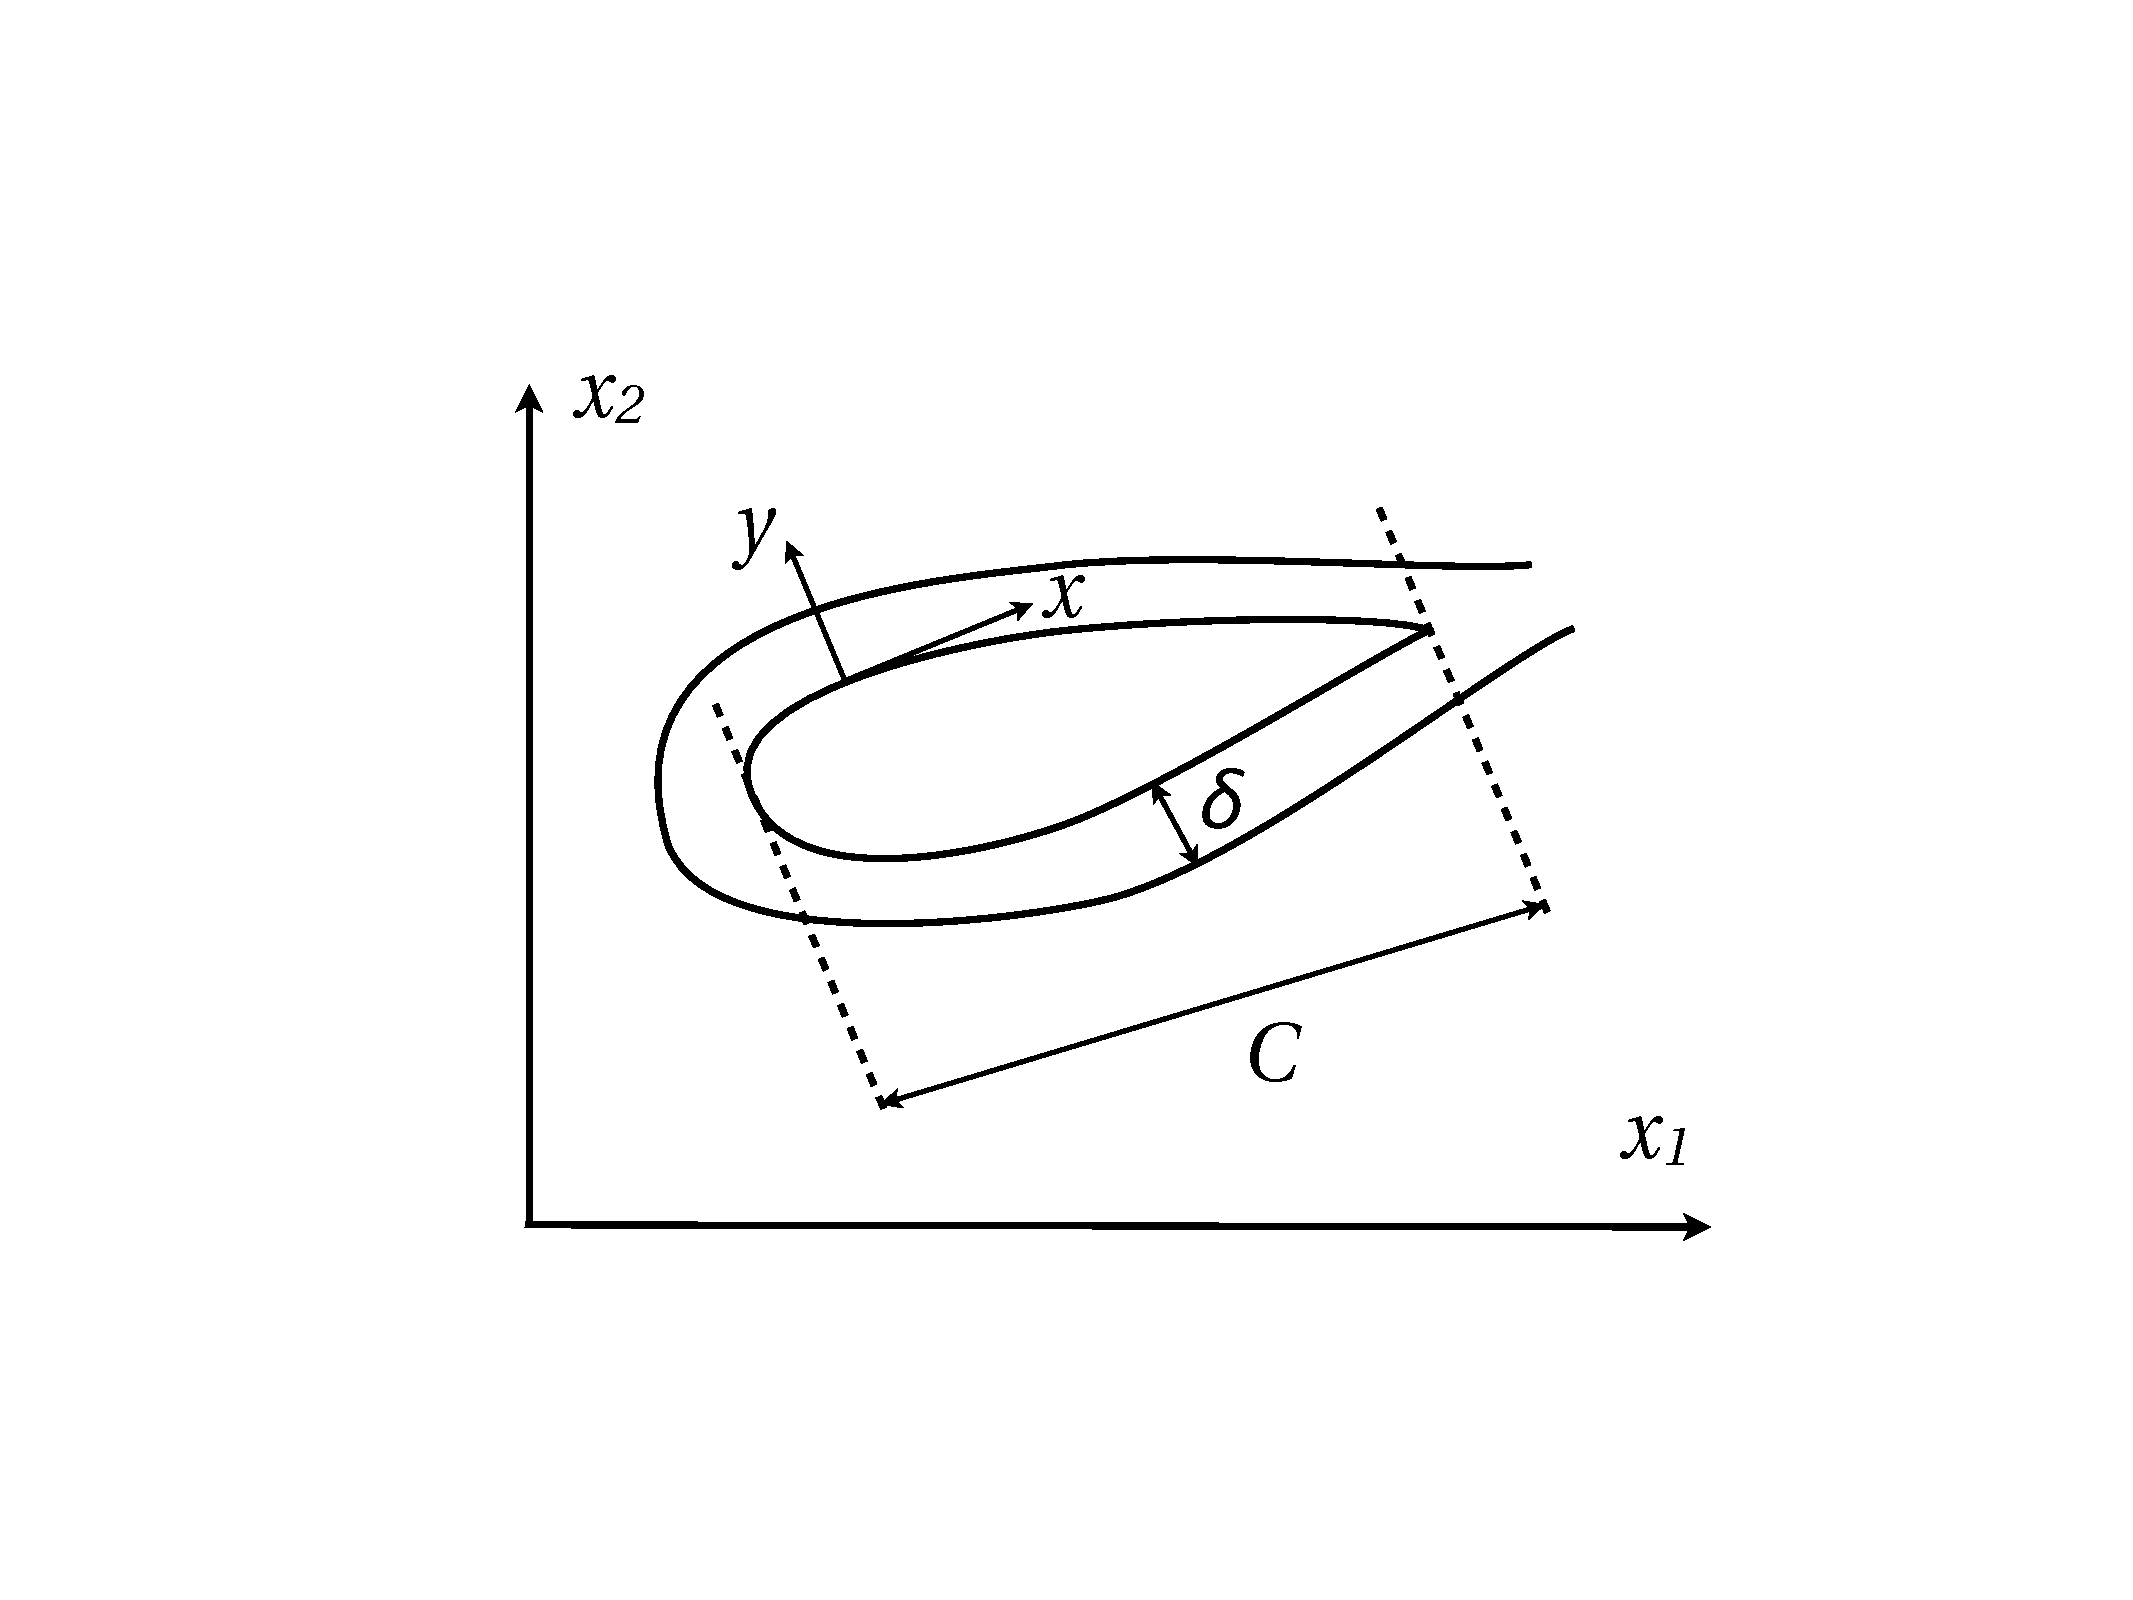
\includegraphics[scale=0.23]{ch5/1}
	\captionof{figure}{}	
	\end{wrapfigure}
	Let's remind that in the introduction we analysed the circumstances in whihch viscous forces can be neglected and the conclusion was that it was caracterized by the Reynold's number. When it is large, it means that viscous forces are small compared to convective inertial forces. Despite the small order of magnitude of viscous forces, they can't be neglected everywhere (walls). This leads us to consider 2 region around a body : 
	\ \\
	\begin{itemize}
		\item[•] \textbf{the distal or outer zone}: wherer the flow is inviscid so viscous forces are negligible (ch3). 
		\item[•] \textbf{the thin, proximal or inner zone}: where viscous stresses may not be neglected, leading to the boundary \textbf{layer} $\mathbf{\delta}$ which is next to a solid wall and a region behind the body called the \textbf{wake} (sillage). \\
	\end{itemize}
	
	We hope that, similarly to the inviscid case where equations simplifies, the case will be here because of the small thickness of the boundary layer. We make a first assumption saying that if $C$ is the caracteristic length of the body in the tengential direction and $\delta$ the one in the normal direction

	\begin{equation}
		when \ Re_C \gg 1 \qquad \Rightarrow \delta \ll C
	\end{equation}
	The whole chapter is based on constant density flows, so the governing equation in 2D are
	
	\begin{equation}
	\begin{aligned}
		&\frac{\D u_1}{\D x_1} + \frac{D u_2}{\D x_2} = 0\\
		&\rho \left[ u_1 \frac{\D u_1}{\D x_1} + u_2 \frac{\D u_1}{\D x_2} \right] = -\frac{\D p}{\D x_1} + \mu \left( \frac{\D ^2 u_1}{\D x_1^2} + \frac{\D ^2 u_1}{\D x_2^2} \right) \\
		&\rho \left[ u_1 \frac{\D u_2}{\D x_1} + u_2 \frac{\D u_2}{\D x_2} \right] = -\frac{\D p}{\D x_2} + \mu \left( \frac{\D ^2 u_2}{\D x_1^2} + \frac{\D ^2 u_2}{\D x_2^2} \right)
	\end{aligned}
	\end{equation}
	
	These equations are for a coordinate system established to study the outer flow. Now as we analyse the flow in a fin layer close to the body it is convinient to rewrite the flow equations in a body fitted curvilinear system where $x$ is the curvilinear coordinate tengent to the body and $y$ the one normal to the body. If we can assume that $\delta \ll R$ which is the body radius of curvature (variable), the transformed curvilinear equations are identical to the original cartesian equations
	
	\begin{equation}
		\begin{aligned}
		&\frac{\D u}{\D x} + \frac{\D v}{\D y} = 0\\
		&\rho \left[ u \frac{\D u}{\D x} + v \frac{\D u}{\D y} \right] = -\frac{\D p}{\D x} + \mu \left( \frac{\D ^2 u}{\D x^2} + \frac{\D ^2 u}{\D y^2} \right) \\
		&\rho \left[ u \frac{\D v}{\D x} + v \frac{\D v}{\D y} \right] = -\frac{\D p}{\D y} + \mu \left( \frac{\D ^2 v}{\D x^2} + \frac{\D ^2 v}{\D y^2} \right)
	\end{aligned}
	\end{equation}
	
	The condition $\delta \ll R$ is the most likely to be violated where R is the smalest, which corresponds to the front of the body. But let's imagine that the condition is fullfilled. In these equations we didin't use $\delta$ so let's rewrite these equations in non-dimensional form by choosing the non-dimensional variables $(\tilde{x}, \tilde{y}, \tilde{u}, \tilde{v}, \tilde{p})$ in such a way that they'll be of order of magnitude 1
	
	\begin{equation}
	\begin{aligned}
		&\tilde{x} = \frac{x}{C} \qquad\qquad  \tilde{u} = \frac{u}{\uinf} \qquad\qquad  \tilde{p} = \frac{C_p}{2} = \frac{p-p_0}{\rho\uinf ^2}\\
		&\tilde{y} = \frac{y}{\delta} \qquad \qquad \ \tilde{v} = \frac{v}{v_\delta (?)} 
	\end{aligned}
	\end{equation}
	
	where for $u$ we know that for the inviscid case we considered $\uinf$ as velocity of the flow on the body and $v$ was null on the body wall so we have a "?". The continuity equation in dimensionless variables will help us 
	
	\begin{equation}
		\frac{\uinf}{C}\frac{\D \tilde{u}}{\D \tilde{x}} + \frac{v_\delta}{\delta}\frac{\D \tilde{v}}{\D \tilde{y}} = 0 \qquad \Rightarrow \underbrace{\frac{\D \tilde{v}}{\D \tilde{y}}}_{\theta (1)} = - \frac{\uinf}{C} \frac{\delta}{v_\delta} \underbrace{\frac{\D \tilde{u}}{\D \tilde{x}}}_{\theta (1)} \qquad \Rightarrow \frac{\uinf}{C} \frac{\delta}{v_\delta} = \theta (1) \Leftrightarrow v_\delta = \theta \left( \frac{\delta \uinf}{C}\right)
	\end{equation}	 
	
	where $\theta (1)$ means order of magnitude 1. We are going to replace $v_\delta = \frac{\delta \uinf}{C}$. We are going to do the same operation for momentum equations. Let's begin with the tengential momentum equation
	
	\begin{equation}
	\begin{aligned}
		&\rho \left[ \frac{\uinf ^2}{C}\tilde{u} \frac{\D \tilde{u}}{\D \tilde{x}} + \frac{\uinf ^2 \cancel{\delta}}{C} \frac{\tilde{v}}{\cancel{\delta}}\frac{\D \tilde{u}}{\D \tilde{y}} \right] = -\rho \frac{\uinf ^2}{C} \frac{\D \tilde{p}}{\D \tilde{x}} + \mu \left( \frac{\uinf}{C^2}\frac{\D ^2 \tilde{u}}{\D \tilde{x}^2} + \frac{\uinf}{\delta ^2}\frac{\D ^2 \tilde{u}}{\D \tilde{y}^2} \right) \\
		\Leftrightarrow \qquad &\rho \frac{\uinf ^2}{C}\left[ \tilde{u} \frac{\D \tilde{u}}{\D \tilde{x}} +  \tilde{v} \frac{\D \tilde{u}}{\D \tilde{y}} + \frac{\D \tilde{p}}{\D \tilde{x}}  \right] =  \mu \frac{\uinf}{\delta ^2} \left( \cancel{\frac{\delta ^2}{C^2}\frac{\D ^2 \tilde{u}}{\D \tilde{x}^2}}+ \frac{\D ^2 \tilde{u}}{\D \tilde{y}^2} \right) \\
	\end{aligned}
	\end{equation}
	
	where we make appear $\frac{\delta ^2}{C^2}$ which is much smaller than one if $Re_C \gg 1$. Because of all the dimensionless variables are of order of magnitude 1 $\theta (1)$ the two constants must be of the same order of magnitude
	
	\begin{equation}
		C\frac{\rho \uinf ^{\cancel{2}}}{C^2} \frac{\delta ^2}{\mu \cancel{\uinf}} = \theta (1) \qquad \Leftrightarrow \left( \frac{\delta}{C}\right)^2 = \theta \left( \frac{\mu}{\rho \uinf C}\frac{1}{Re _C} \right) =  \qquad \Rightarrow \delta = \theta \left(\frac{C}{\sqrt{Re_C}} \right) \ll C
	\end{equation}
	
	which confirms the assumption $\delta \ll C$ when $Re_C\gg 1$. From now we will take $\delta = \frac{C}{\sqrt{Re_C}}$. To conclude, it remains the normal momentum equation 
	
	\begin{equation}
	\begin{aligned}
		&\rho \left[ \frac{\uinf ^2 \delta}{C^2}\tilde{u} \frac{\D \tilde{v}}{\D \tilde{x}} + \frac{\uinf ^2 \delta^{\cancel{2}}}{C^2} \frac{\tilde{v}}{\cancel{\delta}}\frac{\D \tilde{v}}{\D \tilde{y}} \right] = -\rho \frac{\uinf ^2}{\delta} \frac{\D \tilde{p}}{\D \tilde{y}} + \mu \left( \frac{\uinf \delta}{C^3}\frac{\D ^2 \tilde{v}}{\D \tilde{x}^2} + \frac{\uinf\delta}{C\delta ^{2}}\frac{\D ^2 \tilde{v}}{\D \tilde{y}^2} \right) \\
		\Leftrightarrow\qquad &\rho \frac{\uinf ^2\delta}{C^2}\left[ \tilde{u} \frac{\D \tilde{v}}{\D \tilde{x}} +  \tilde{v} \frac{\D \tilde{v}}{\D \tilde{y}}  \right] = - \rho\frac{\uinf ^2}{\delta} \frac{\D \tilde{p}}{\D \tilde{y}} +  \mu \frac{\uinf }{C\delta} \left( \cancel{\frac{\delta ^2}{C^2}\frac{\D ^2 \tilde{v}}{\D \tilde{x}^2}}+ \frac{\D ^2 \tilde{v}}{\D \tilde{y}^2} \right) \\
		\Leftrightarrow\qquad  &\rho \uinf ^2\left[ \tilde{u} \frac{\D \tilde{v}}{\D \tilde{x}} +  \tilde{v} \frac{\D \tilde{v}}{\D \tilde{y}}  \right] = - \rho\uinf^2\left(\frac{C}{\delta}\right) ^2 \frac{\D \tilde{p}}{\D \tilde{y}} +  \mu\uinf \underbrace{\left(\frac{C}{\delta}\right)^2}_{Re_C = \rho\frac{C\uinf}{\mu}} \frac{1}{C} \frac{\D ^2 \tilde{v}}{\D \tilde{y}^2}\\
		\Leftrightarrow\qquad  &\rho \uinf ^2\left[ \tilde{u} \frac{\D \tilde{v}}{\D \tilde{x}} +  \tilde{v} \frac{\D \tilde{v}}{\D \tilde{y}}  \right] = - \rho\uinf^2\left(\frac{C}{\delta}\right) ^2 \frac{\D \tilde{p}}{\D \tilde{y}} +  \frac{\cancel{\mu}\uinf}{\cancel{C}} \rho\frac{\cancel{C}\uinf}{\cancel{\mu}} \frac{\D ^2 \tilde{v}}{\D \tilde{y}^2}\\
				\Leftrightarrow\qquad  &\underbrace{\tilde{u} \frac{\D \tilde{v}}{\D \tilde{x}} +  \tilde{v} \frac{\D \tilde{v}}{\D \tilde{y}} -  \frac{\D ^2 \tilde{v}}{\D \tilde{y}^2}}_{\theta (1)} = - \left(\frac{C}{\delta}\right) ^2 \frac{\D \tilde{p}}{\D \tilde{y}} \qquad \Rightarrow \frac{\D \tilde{p}}{\D \tilde{y}} = \theta \left(\frac{\delta}{C}\right) ^2 
	\end{aligned}
	\end{equation}

	where we see that the pressure gradient accross the boundary layer normal to the wall cannot be of order of magnitude 1 but of that of $\left(\frac{\delta}{C}\right) ^2$ which is \textbf{negligible}

	\begin{equation}
		\tilde{p}(\tilde{x}, \tilde{y}) = \tilde{p}_e (\tilde{x}) \qquad \Rightarrow p(x,y) = p_e(x) 
	\end{equation}

	where $p_e(x)$ is the outer inviscid flow pressure distribution. The pressure variation inside the boundary layer beeing null, the pressure inside is equal to the outer pressure distribution computed on the wall. The pression is no longer an unknown. The final form of the equations in the boundary layer are 

	\begin{equation}
	\begin{array}{l|l}
		\frac{\D \tilde{u}}{\D \tilde{x}} + \frac{\D \tilde{v}}{\D \tilde{y}} = 0	 & 	\quad\frac{\D u}{\D x} + \frac{\D v}{\D y} = 0\\
	 		\tilde{u} \frac{\D \tilde{u}}{\D \tilde{x}} +  \tilde{v} \frac{\D \tilde{u}}{\D \tilde{y}} = -\frac{d \tilde{p}_e}{d \tilde{x}}	+ \frac{\D ^2 \tilde{u}^2}{\D \tilde{y}^2}\quad & 	\quad	 \rho \left[ u \frac{\D u}{\D x} + v \frac{\D u}{\D y} \right] = -\frac{d p_e}{d x} + \mu \frac{\D ^2 u}{\D y^2}\\
	 		\tilde{p}(\tilde{x}, \tilde{y}) = \tilde{p}_e (\tilde{x}) 	&\quad p(x,y) = p_e(x) 
	\end{array}
	\end{equation}
	
	So it means that if we replace the third equation in the second, we end up with a system of two equations and two unknowns. We also see that the geometry of the body does not appear at all in the equations since we assumed that $\delta \ll R$. The boundary layer is only sensitive the pressure distribution.
	

\section{Zero-pressure gradient (flat plate) boundary layer}
	\begin{wrapfigure}[6]{l}{6cm}
	\vspace{0mm}
	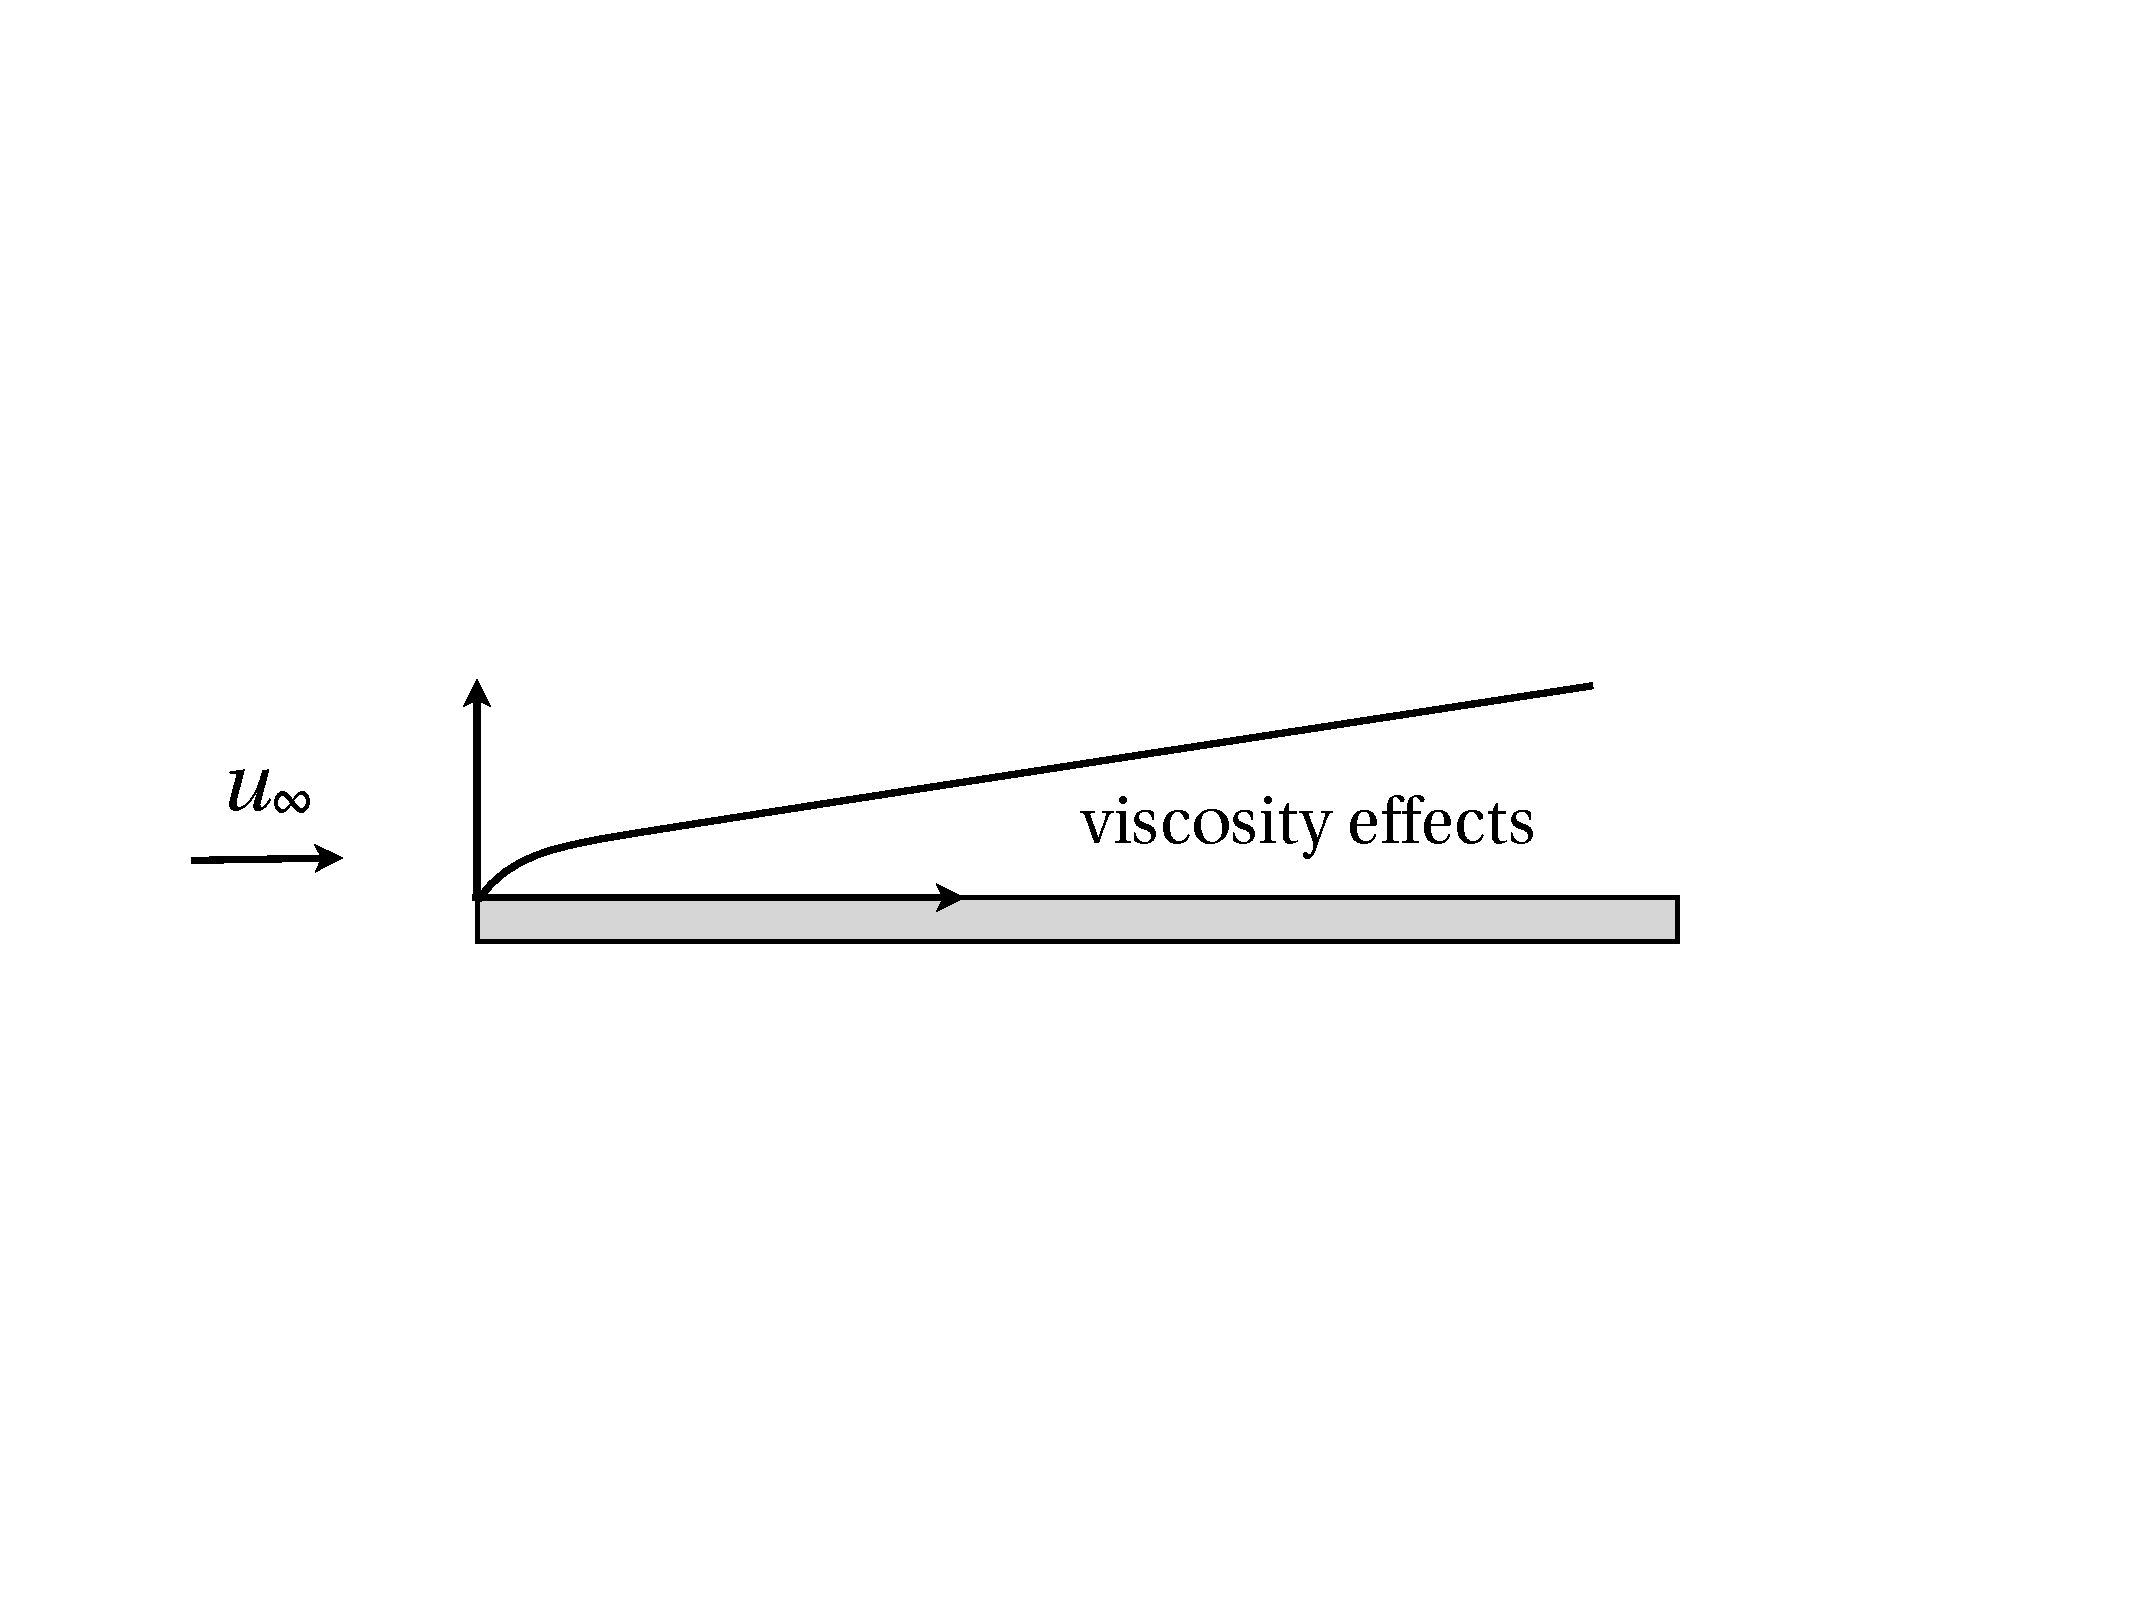
\includegraphics[scale=0.23]{ch5/2}
	\captionof{figure}{}	
	\end{wrapfigure}
	We want to solve the simpliest problem using this when there is no pressure gradient. This correspond to a uniform flow over a flat plate of 0 thickness. The coordinate system is the cartesian one and the outer flow is the uniform flow because the flat plate does not perturb the flow. So for the inviscid flow 
	
	\begin{equation}
		u = \uinf \qquad v = 0 \qquad p = p_\infty \qquad \Rightarrow p_e(x) = p_\infty \Rightarrow \frac{dp_e}{dx} = 0
	\end{equation}
	
	\newpage
	The simplified equations and the initial condition IC and boundary conditions BC are
	
	\begin{equation}
	\begin{aligned}
		&\frac{\D u}{\D x} + \frac{\D v}{\D y} = 0\\
		&u \frac{\D u}{\D x} + v \frac{\D u}{\D y} = \nu \frac{\D ^2 u}{\D y^2}
	\end{aligned}	
	\qquad
	\begin{aligned}
	&IC: u(0,y) = \uinf\\
	&BC: u(x,0) = v(x,0) = 0 \mbox{ (non-slip)}
	\end{aligned}
	\end{equation}
	
	Then we have also the matching boundary conditions that says to the edge of the boundary layer, the velocity should tend to its inviscid value
	
	\begin{equation}
		\lim _{y\rightarrow \infty} u(x,y) = u_e(x) = u^{inv}(x,0) = \uinf 
	\end{equation}
	the far field limit of the boundary flow should be equal to the inner limit of the outer inviscid flow. So the solution at $\infty$ of the boundary flow should be equal to the solution at 0 of the inviscid flow. This is the matching condition for the tengential velocity and not the normal velocity. We are looking solutions $u(x,y)$ and $v(x,y)$. We'll try to represent the sollution to have an idea of how to find it, for $u(x,y)$ in a 3 dimentional coordinate system $x, y, u$. Following IC, when $x=0$, $u = \uinf$ and $y = 0, u=0$. We see that there is a jump, a discontinuity when $x=0=y$ (\autoref{fig:5.3}).\\
	
	 Another way to represent is to plot $y$ in function of $u$ for various axis (positions x). We already know that $u = \uinf$ in the far field and it start from 0 for all axis. If we look at our boundary profile, we know that $\delta$ is increasing with x, meaning that velocity will vary slower along $y$ for increasing $x$ leading to \autoref{fig:5.4}. These last curves have the same shape, such that we can maybe contract them on a same curve. 
	 
		 \begin{center}
		 \begin{minipage}{0.28\textwidth}
	 		\begin{center}
	 		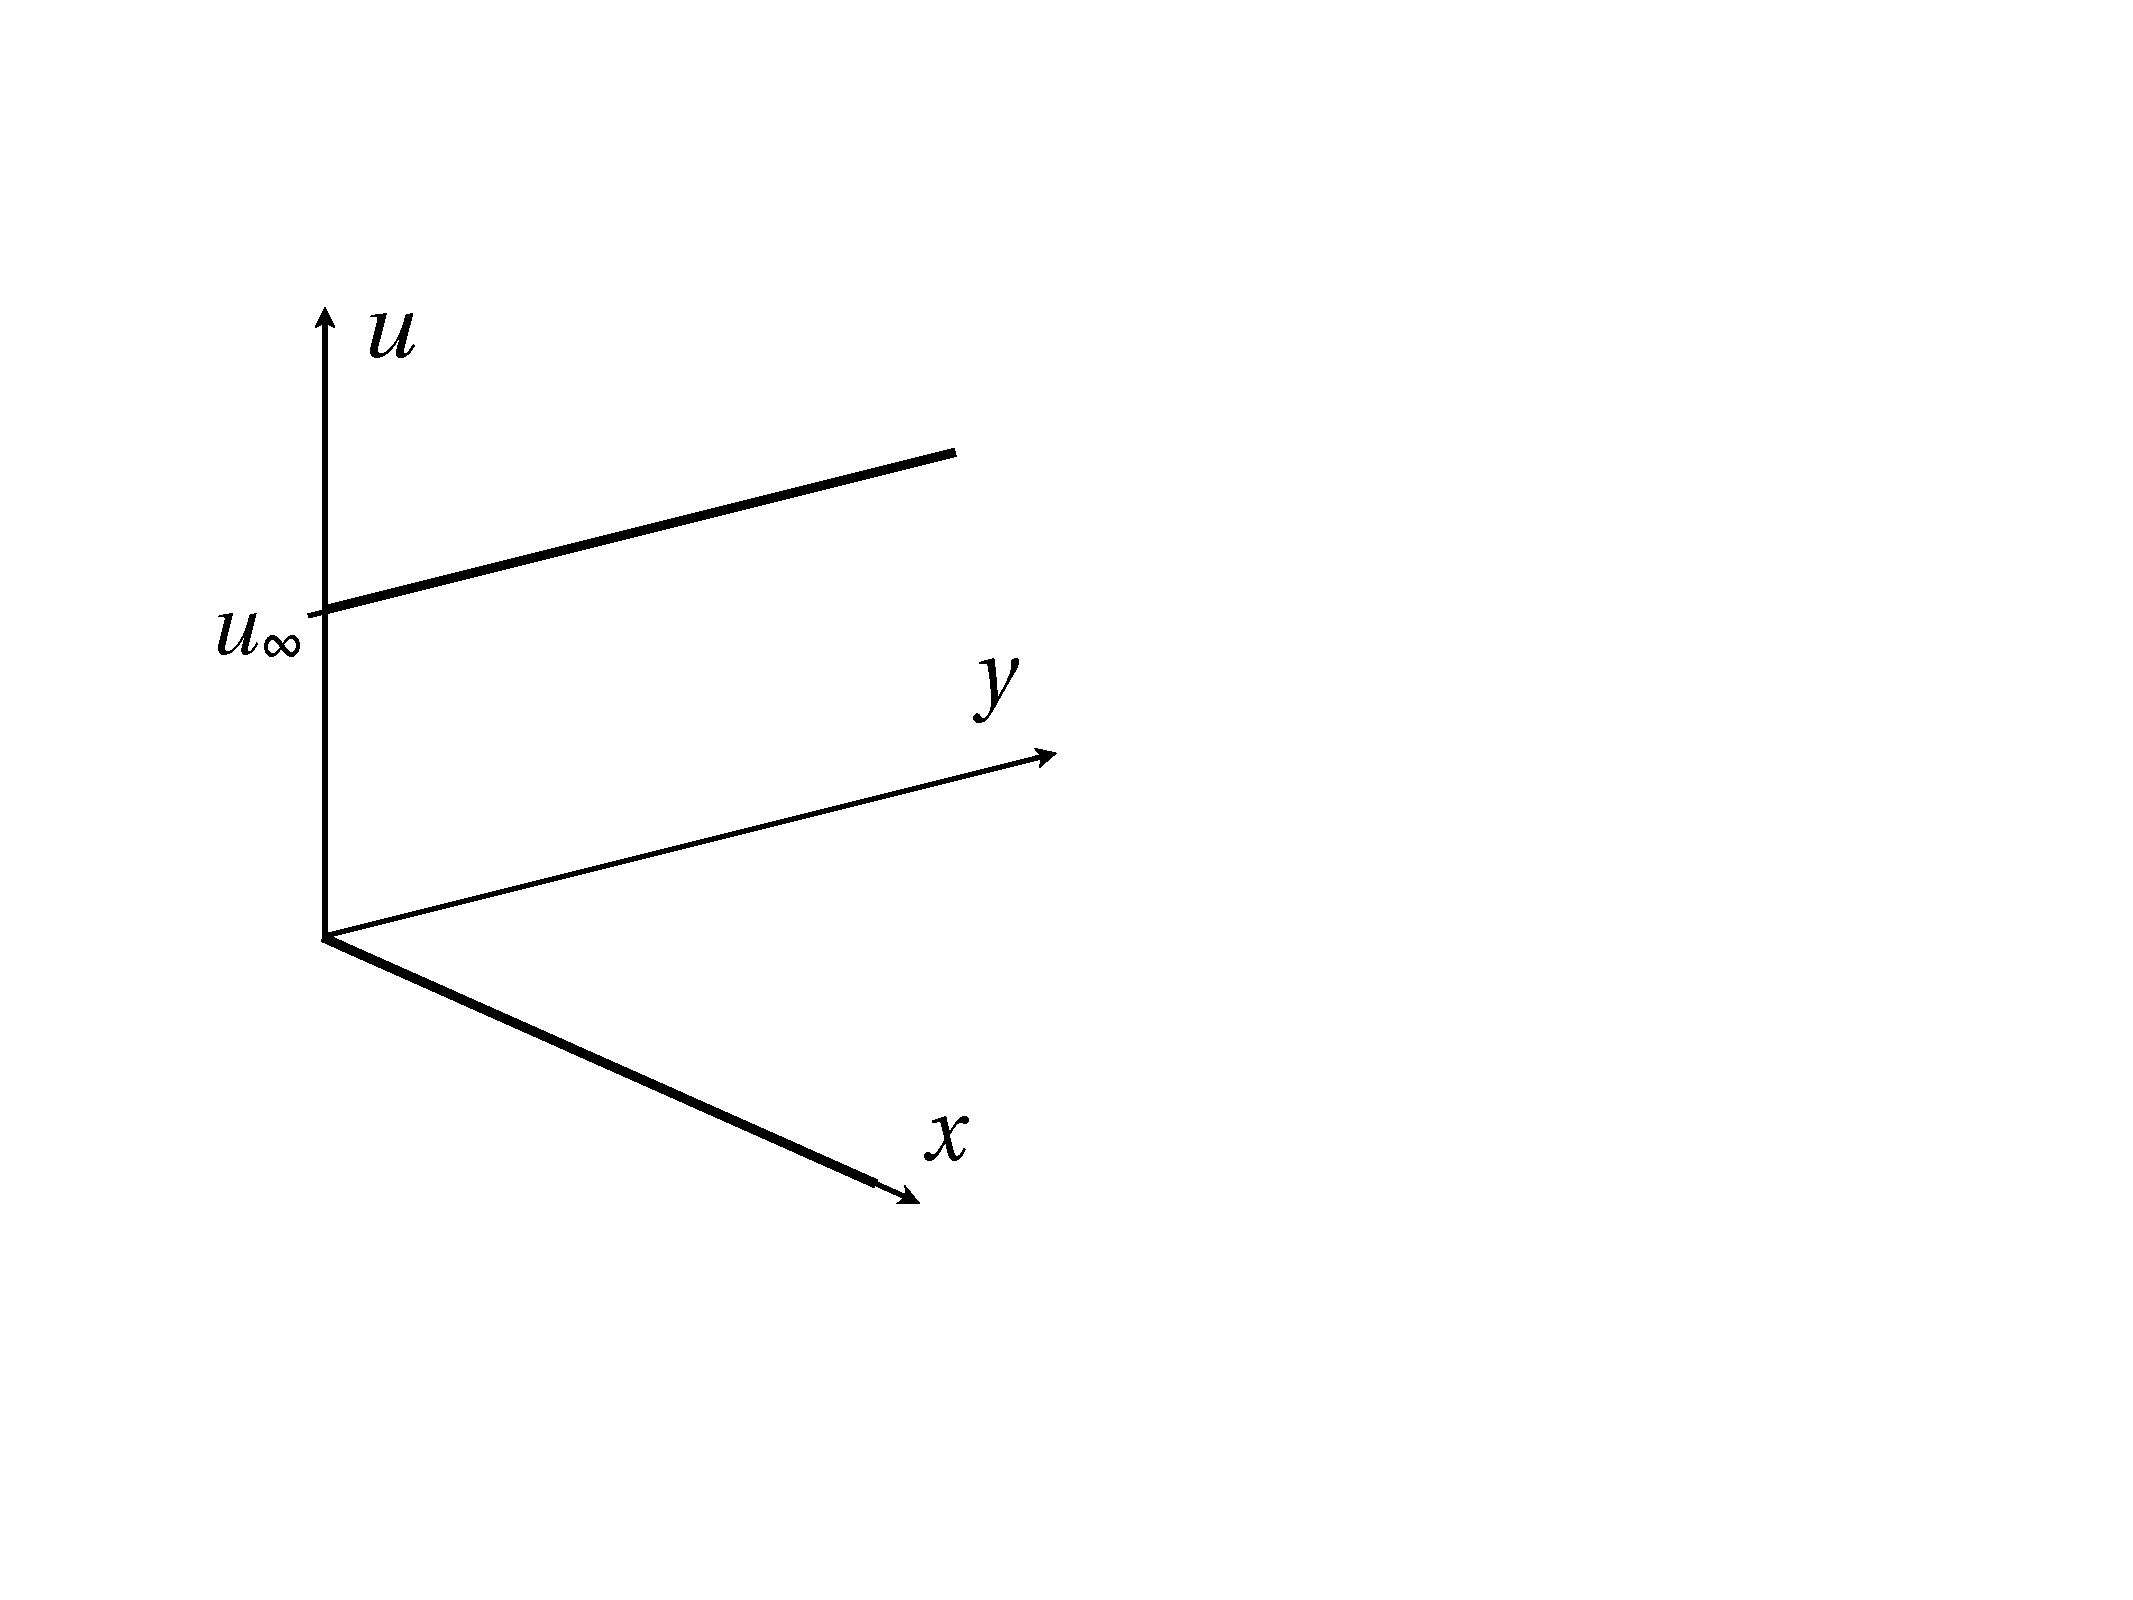
\includegraphics[scale=0.24]{ch5/3}
	 		\captionof{figure}{}
	 		\end{center}
	 		\label{fig:5.3}
	 \end{minipage}
	 	 \begin{minipage}{0.4\textwidth}
			 \begin{center}
			 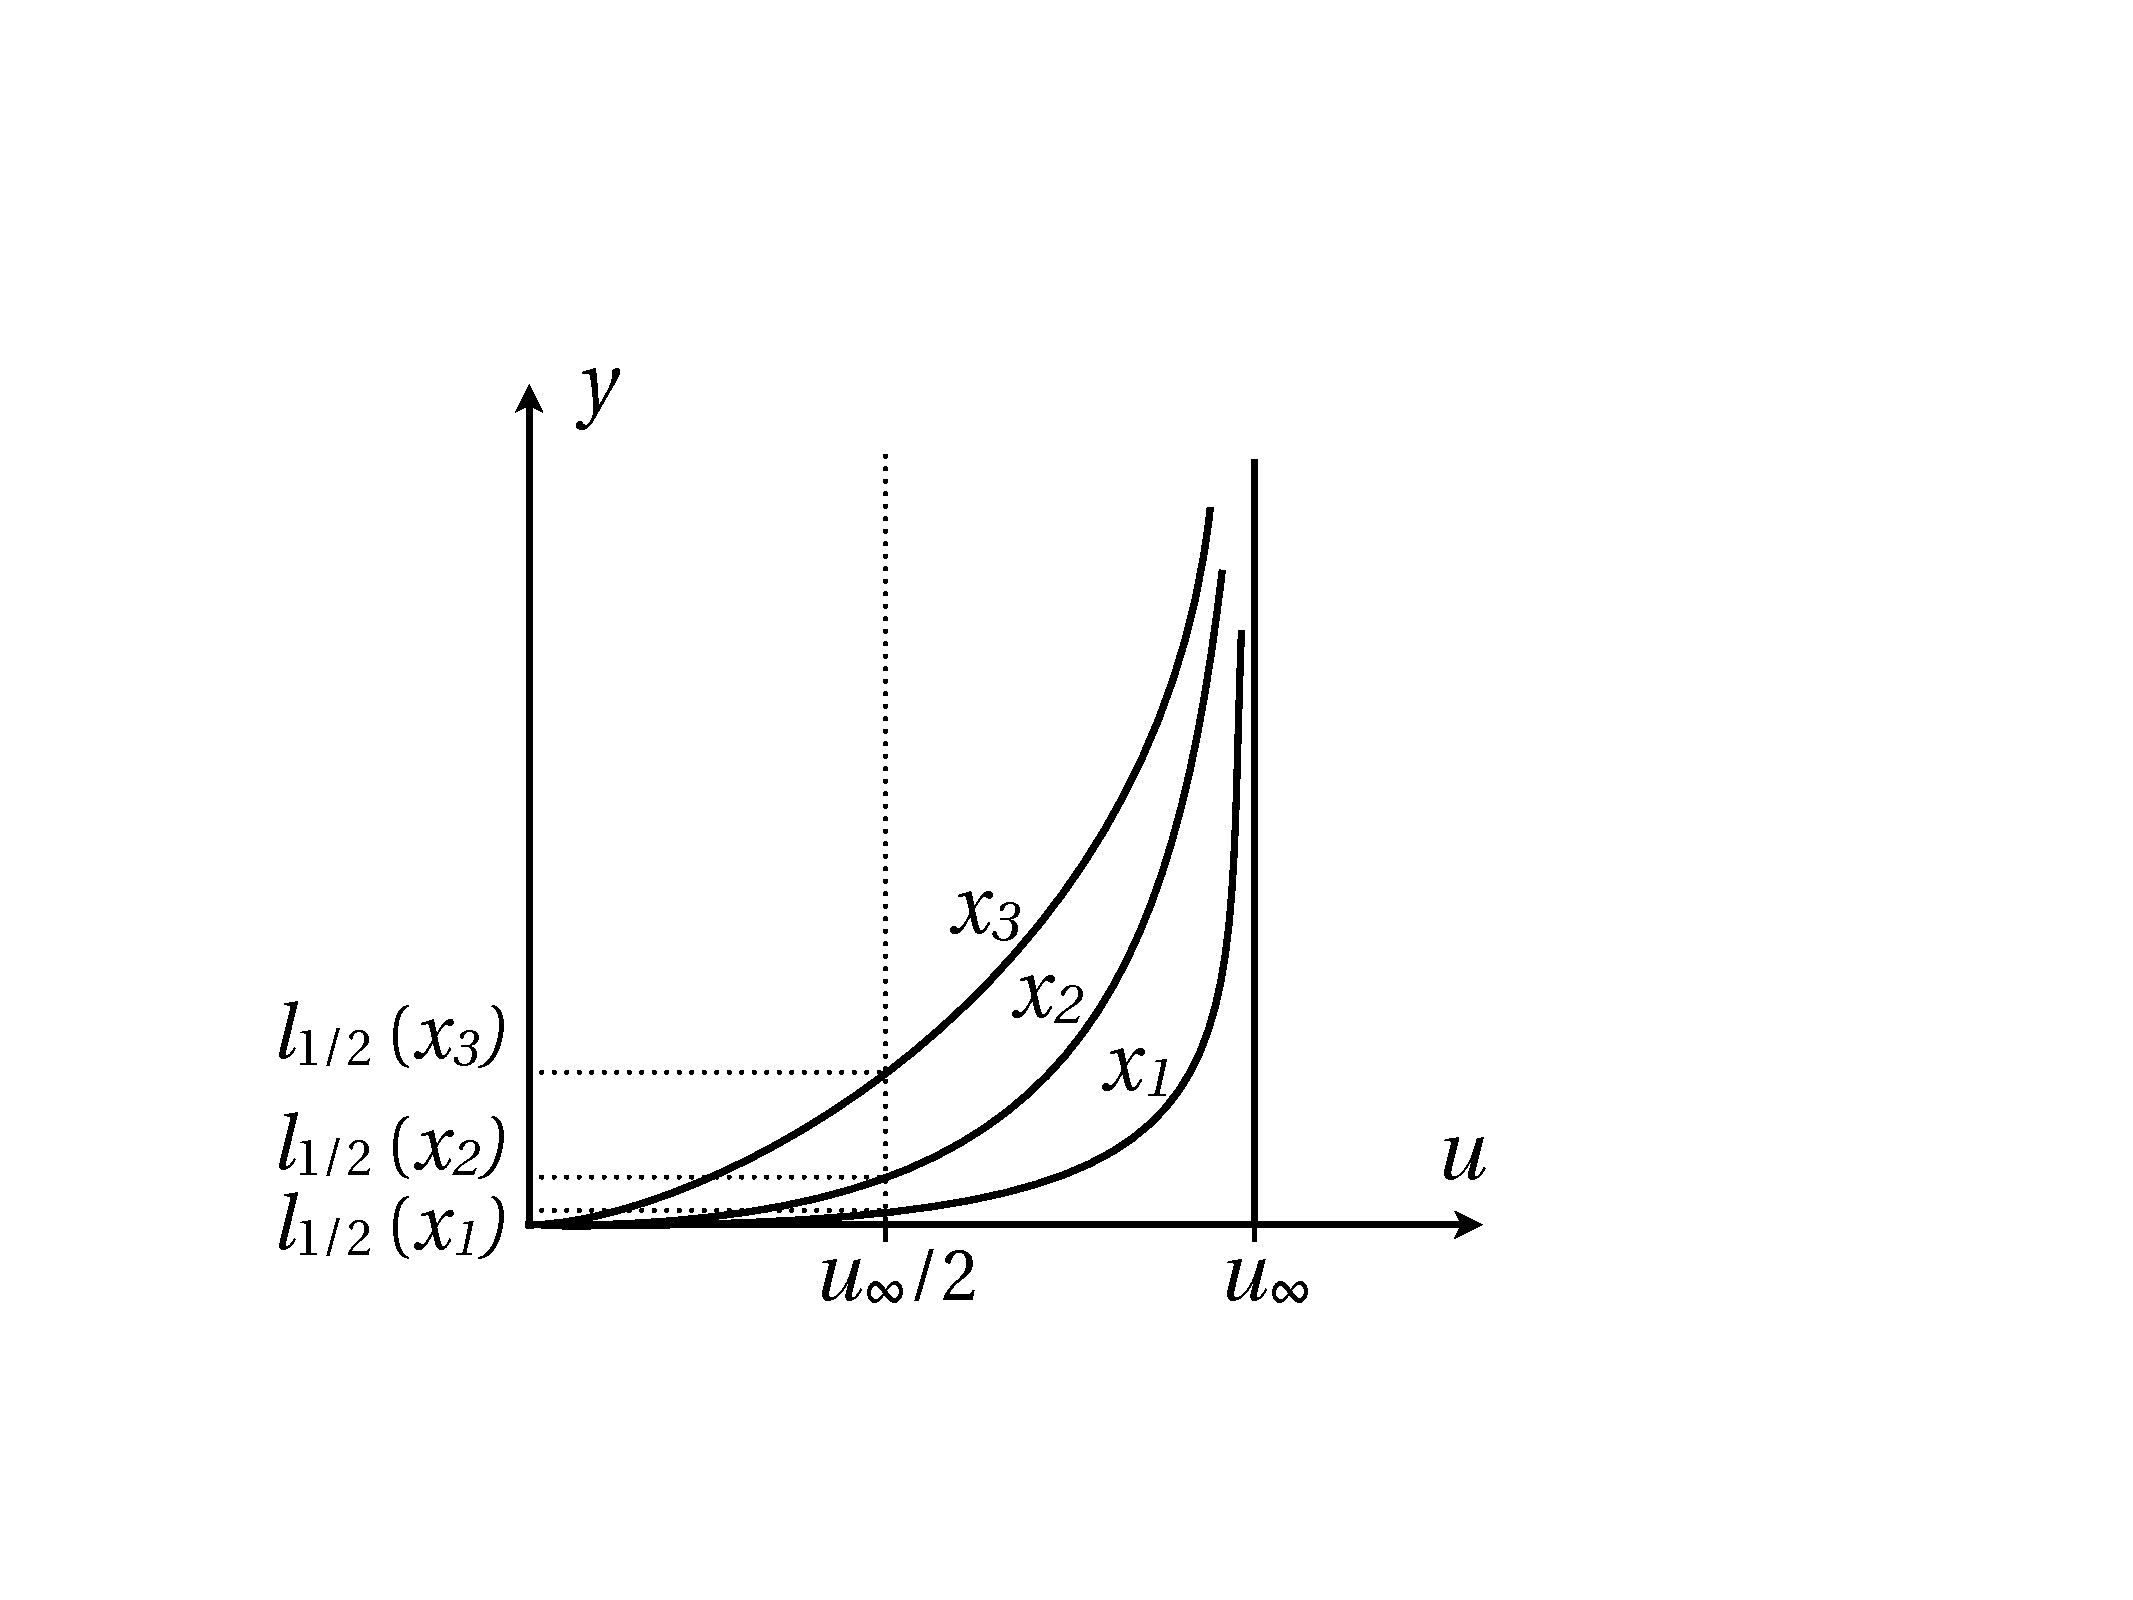
\includegraphics[scale=0.24]{ch5/4} 
			 \captionof{figure}{}
			 \end{center}
	 		\label{fig:5.4}
	 \end{minipage}
	 	 \begin{minipage}{0.3\textwidth}
	 	 	\begin{center}
	 	 	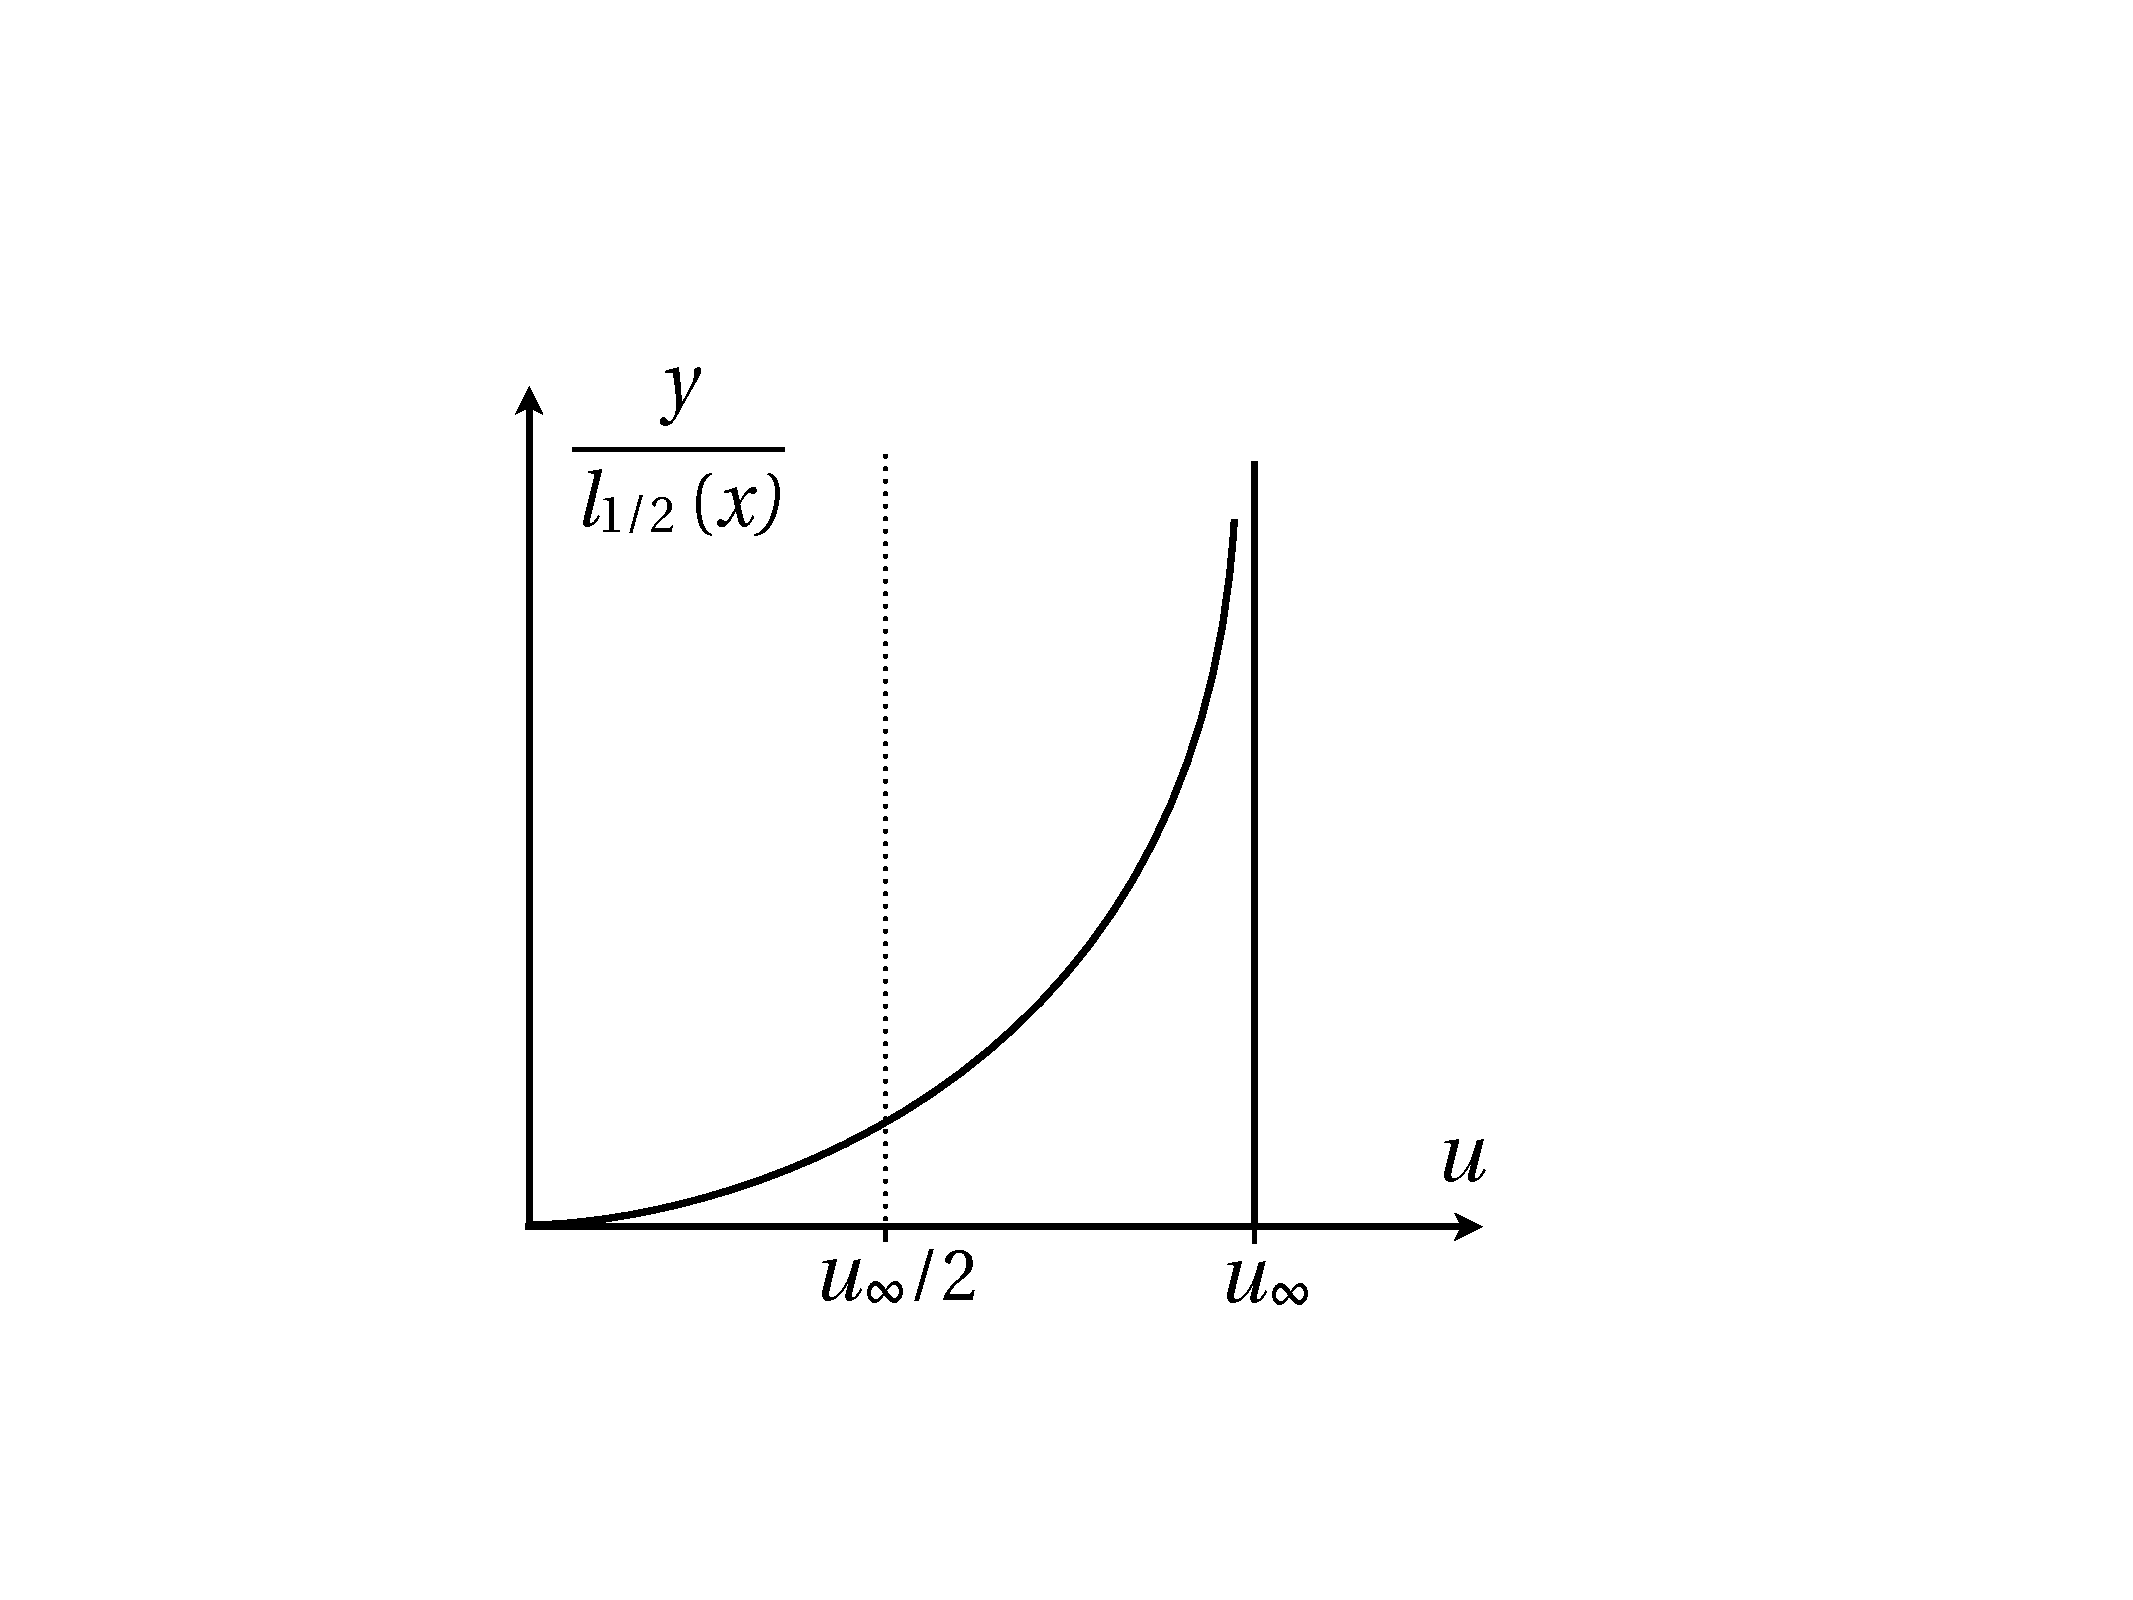
\includegraphics[scale=0.235]{ch5/5}
	 		 \captionof{figure}{}
	 	 	\end{center}
	 		\label{fig:5.5}
	 \end{minipage}
		 \end{center}


	 Let's take a value $\uinf /2$ with the half velocity thickness $l_{1/2}(x)$. If we repllot $u/\uinf$ in function of $y/l_{1/2}(x)$, we know that at $\uinf /2$ we will have 1 and 0 at 0. If we assume that all the curves have the same shape, they all pass from these 2 points as represented on \autoref{fig:5.5}. This is called the \textbf{self similarity assumption} and we'll have to check it.  		 \\
		 
	\begin{wrapfigure}[8]{l}{5cm}
	\vspace{-5mm}
	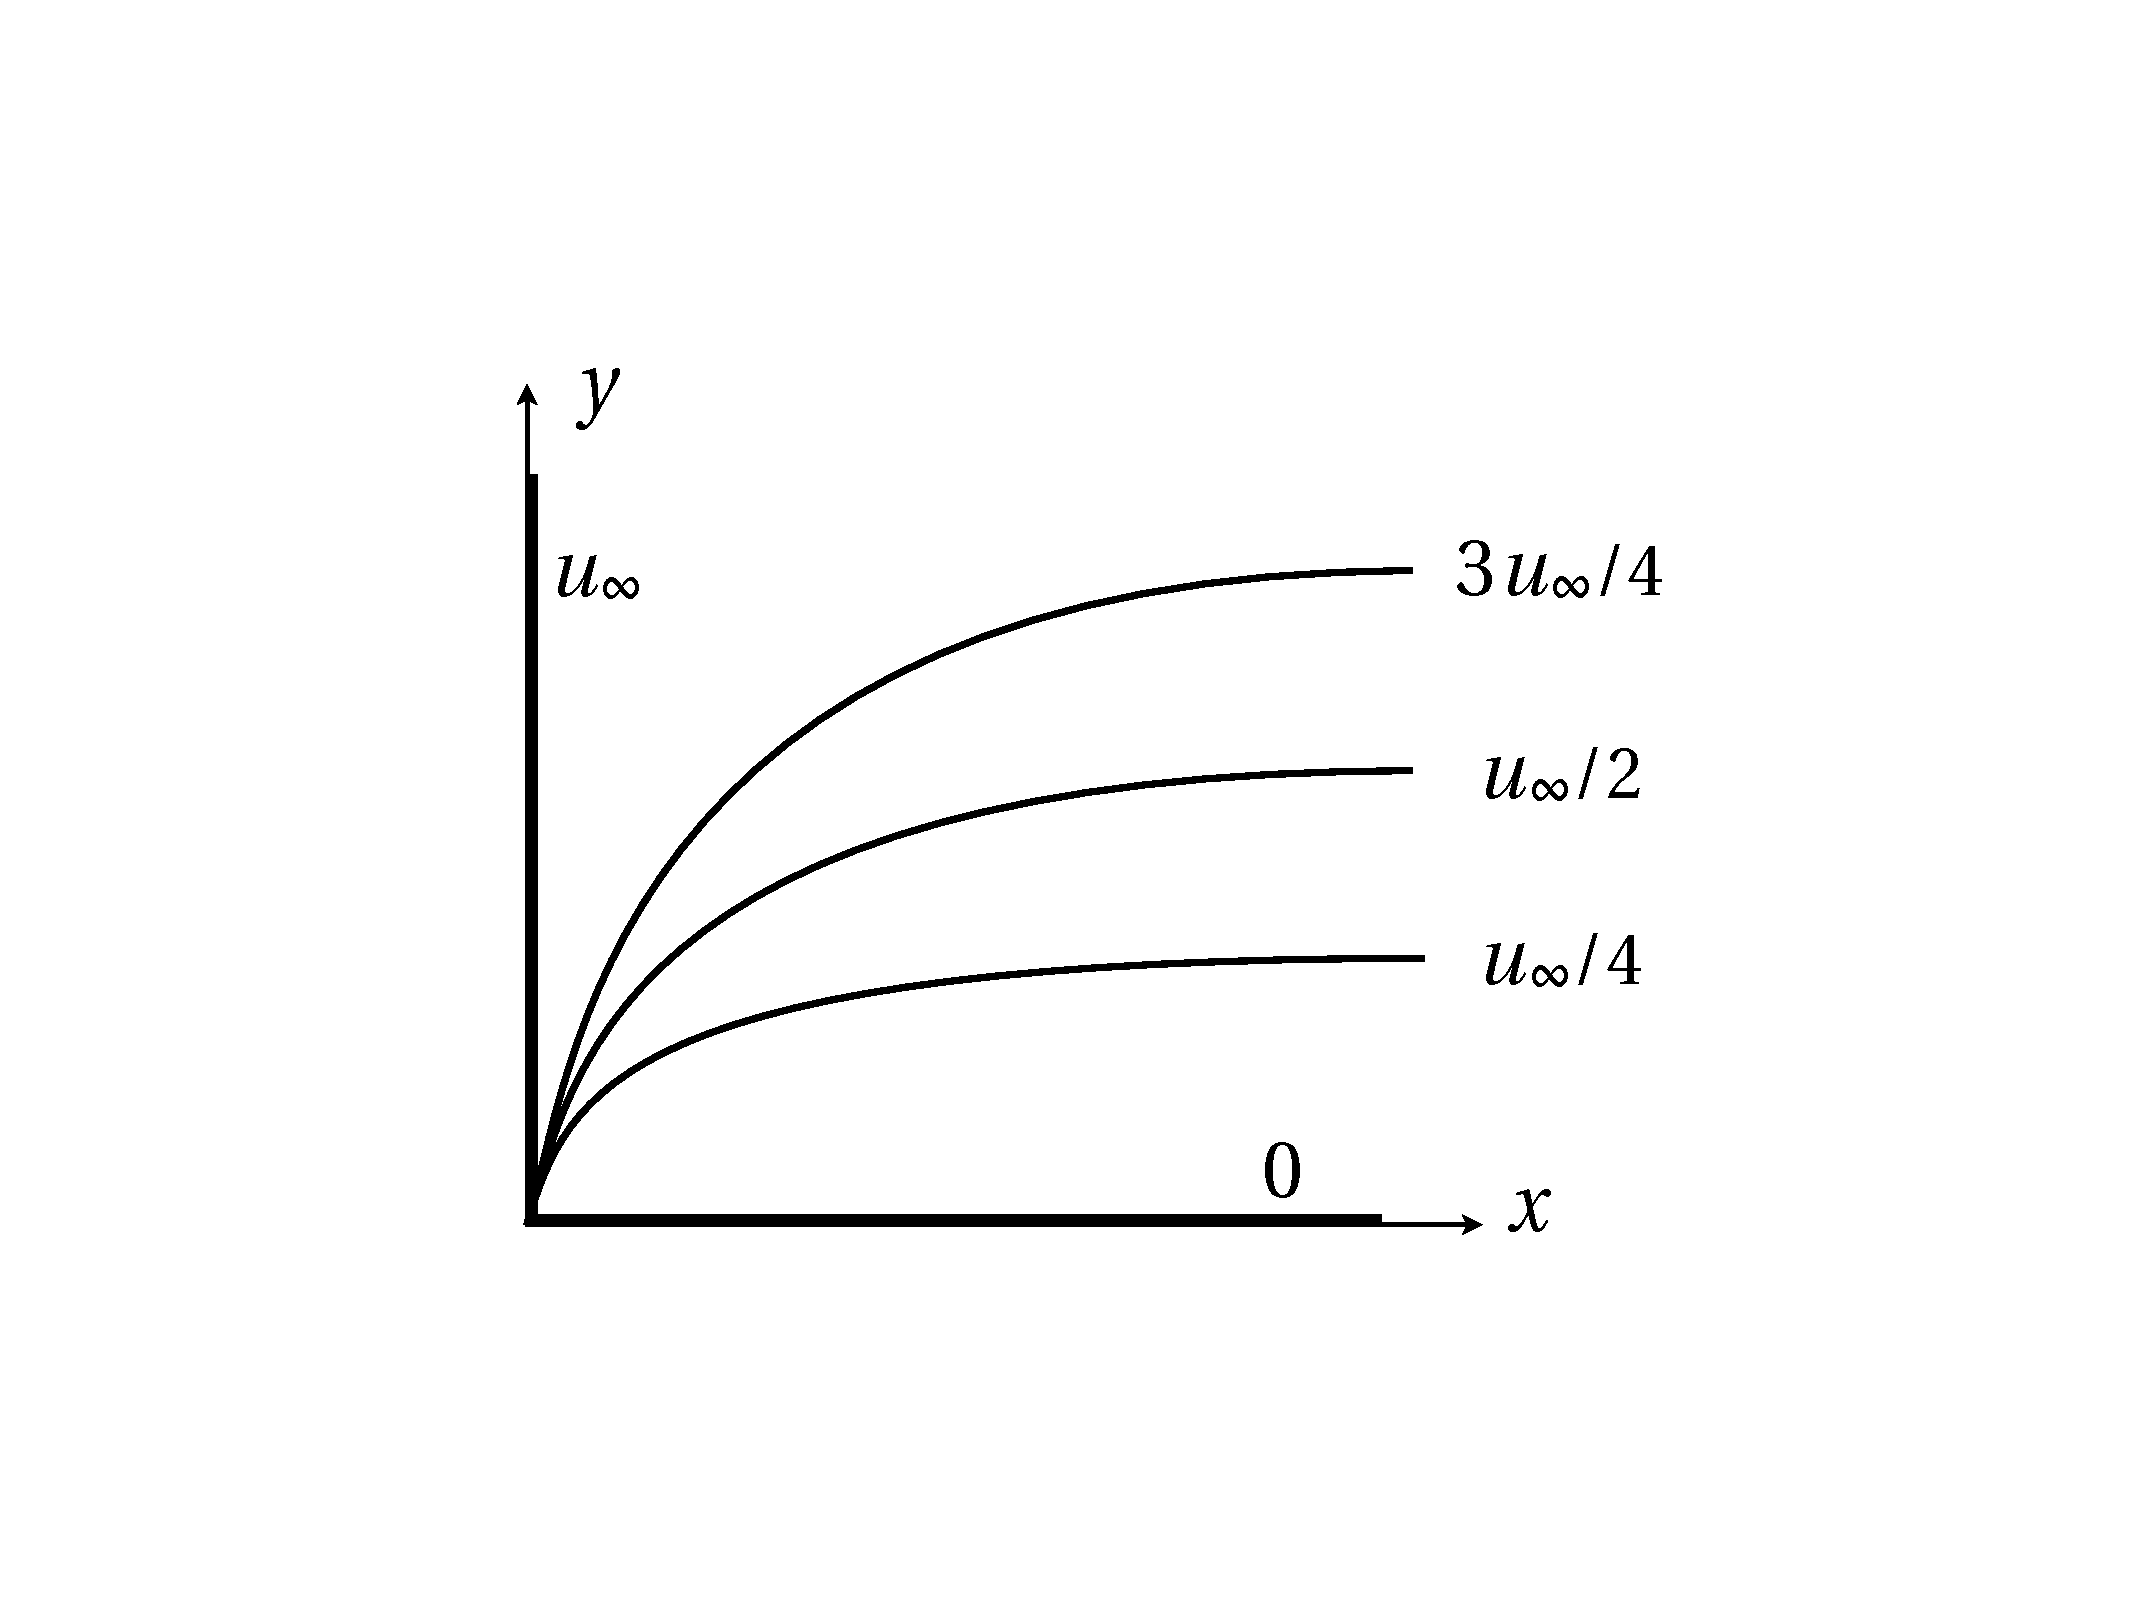
\includegraphics[scale=0.23]{ch5/6}
	\captionof{figure}{}	
	\label{fig:5.6}
	\end{wrapfigure}
	In order to verify the assumption, let's first represents \autoref{fig:5.4} as \autoref{fig:5.6}, this is equivalent to plot the \textbf{contour lines}. The contour $u=\uinf$ is vertical and $u=0$ horizontale, $u=\uinf /2$ will have the equation $y = l_{1/2}(x)$ by definition. If \autoref{fig:5.5} is valid, we will have for example for $\frac{u}{\uinf} = 0.1$, $\frac{y}{l_{1/2}(x)} = c_{0.1}$. So the contour line $u = 0.1 \uinf$ has as equation $y = c_{0.1}l_{1/2}(x)$. We see that in fact the self similarity assumption implies that the contour lines are stretched expression of the same function. 
	
	\newpage
	
	\subsubsection{Coordinate transformation}
		Let's imagine that we make a change of variables 

		\begin{equation}
			\xi = x \qquad \eta = \frac{y}{l_{1/2}(x)} = \frac{y}{l(x)}.
			\label{eq:5.14}
		\end{equation}
		By the way, we use the value at $1/2$ but we could take what we want, the only change is the constant. Now if we plot $\eta$ in function of $\xi$, the self similarity assumption in the case of contour plot means that if all velocity profile have the same value of $x$ so the same $\xi$. It means that the contour lines will be horizontal lines in the transformed variables. So if the transformation induces no variation along $\xi$
		
		\begin{equation}
			u(x,y) \rightarrow u(\cancel{\xi} , \eta ) \qquad \Rightarrow \frac{u}{\uinf} = g(\eta).
		\end{equation}
		
		The solution only depends on $\eta$. This is an assumption and we have to check. For that we have to make the change of variables in the equations using the relation 
		
		\begin{equation}
		\begin{aligned}
		&\forall \varphi (x,y) = \hat{\varphi}(\xi (x,y), \eta (x,y)) \\
			\frac{\partial \varphi}{\partial x} = \frac{\partial \hat{\varphi}}{\partial \xi} 	\frac{\partial \xi}{\partial x} &+ \frac{\partial \hat{\varphi}}{\partial \eta} \frac{\partial \eta}{\partial x} \qquad and \qquad
			\frac{\partial \varphi}{\partial y} = \frac{\partial \hat{\varphi}}{\partial \xi} \cancel{\frac{\partial \xi}{\partial y}} + \frac{\partial \hat{\varphi}}{\partial \eta} \frac{\partial \eta}{\partial y}.
		\end{aligned}
		\end{equation}
		
		We can now compute the derivative of the velocities
		
		\begin{equation}
		\begin{aligned}
			&\frac{\D u}{\D x} = \cancel{\frac{\D (\uinf g)}{\D xi}} \frac{\D xi}{\D x} + \underbrace{\frac{\D (\uinf g)}{\D \eta}}_{\uinf g'} \underbrace{\frac{\D \eta}{\D x}}_{-\frac{y}{l^2(x)}\frac{dl}{dx}} = - \uinf g'(\eta)\frac{y}{l^2(x)}\frac{dl(x)}{dx} = - \uinf g'(\eta)\eta \frac{1}{l(\xi)} \frac{dl(\xi)}{d\xi}\\
			&\frac{\D u}{\D y} = \frac{\D \uinf g}{\D \eta} \frac{1}{l(\xi)} = \uinf \frac{g'}{l(\xi)} \qquad and \qquad \frac{\D ^2 u}{\D y }= \uinf \frac{g''}{l^2(\xi)}
		\end{aligned}
		\label{eq:5.17}
		\end{equation}
		
		\subsubsection{Continuity equation}
			Let's integrate and replace by what we expressed ($\zeta = z/l(\xi), z \equiv y, \zeta \equiv \eta$)
	
			\begin{equation}
			\begin{aligned}
				\frac{\D v}{\D y} =- \frac{\D u}{\D x} = \uinf g'(\eta) \frac{\eta}{l(\xi)} \frac{dl(\xi)}{d\xi} \qquad \Leftrightarrow &v(x,y) - v(x,0) = \uinf \int _0 ^y g'(\zeta) \frac{\zeta}{l(\xi)} \frac{dl(\xi)}{d\xi} \, dz\\
				\Leftrightarrow &v(x,y) = \uinf \frac{dl(\xi)}{d\xi} \underbrace{\int _0 ^\eta g'(\zeta) \zeta  \, d\zeta}_{F(\eta)}
			\end{aligned}	
			\end{equation}
			where if we integrate by part we find $F(\eta) = \eta g - \int g\, d\zeta = \eta f' - f(\eta)$. This implies that \eqref{eq:5.17} becomes 
			
			\begin{equation}
				\frac{\D u }{\D x} = - \uinf f''\eta \frac{1}{l(\xi)} \frac{dl}{d\xi} \qquad \frac{\D u}{\D y} = \uinf \frac{f''}{l} \qquad \frac{\D ^2 u}{\D y }= \uinf \frac{f'''}{l^2}.
			\end{equation}
			
			A first conclusion is that the same similarity of the tengential velocity profile implies a same similarity of the normal velocity profile in the form
			
			\begin{center}
			\theor{
			\begin{equation}
				v = \uinf \frac{dl}{d\xi}(\eta f' - f). 
				\label{eq:5.20}
			\end{equation}
			}
			\end{center}
			
		\subsubsection{Momentum equation}
			We know that $u = \uinf g = \uinf f'$, so the continuity equation becomes
			
			\begin{equation}
			\begin{aligned}
				&\underbrace{\uinf f' \left(  - \uinf f''\eta \frac{1}{l(\xi)} \frac{dl}{d\xi} \right)} + \uinf \frac{dl}{d\xi}(\underbrace{\eta f'} - f) \uinf \frac{f''}{l} = \nu \uinf \frac{f'''}{l^2} \\
				\Leftrightarrow  &- \uinf ^2 \frac{dl}{ld \xi} ff''' = \frac{  \nu \uinf f''}{l^2} \qquad \Leftrightarrow - \uinf ^{\cancel{2}} \frac{dl}{\cancel{l}d \xi} ff'' \frac{l^{\cancel{2}}}{\nu \cancel{\uinf}} = f'''\\
				\Leftrightarrow &-\frac{\uinf l}{\nu} \frac{dl}{d\xi} ff'' = f'''
			\end{aligned}
			\end{equation}
			
			At this stage, we can already conclude something about the validity of the self similarity assumption. Indeed, $l$ is function of $\xi$, $f$ a function of $\theta$, if we bring all $f$ to the right member, we have an equality between a function of $\xi$ and a function of $\eta$. The only way for these to be equal, and so for the assumption to hold, is for the expression to be a \textbf{constant}
			
			\begin{center}
			\theor{
			\begin{equation}
				\frac{\uinf l}{\nu}\frac{dl}{d\xi} = cst \qquad f''' + ff'' = 0
				\label{eq:5.22}
			\end{equation}
			}
			\end{center}
			
			The $l$ is chosen arbitrary so we can choose the constant as wish. We take $cst = 1$. Notice that we can write the last equation in terms of $Re$ as 
			
			\begin{equation}
				Re_l \frac{dl \frac{\uinf}{\nu}}{d\xi \frac{\uinf}{\nu}} = Re_l \frac{dRe_l}{dRe_\xi} = 1 \qquad \Leftrightarrow Re_l^2 = 2 Re_\xi + \cancel{Re_{l_0}^2}.
				\label{eq:5.23}
			\end{equation}
			
			We can easely solve \eqref{eq:5.22}
			
			\begin{equation}
				\frac{\uinf}{\nu}\frac{\frac{dl^2}{2}}{d\xi} = 1 \qquad \Leftrightarrow l^2 = \frac{2\nu}{\uinf} \xi + \cancel{l_0^2} \qquad \Leftrightarrow l = \frac{\sqrt{2}x}{\sqrt{Re_x}}
			\end{equation}
			
			The caracteristic length scale $l_0$ appearing in the equations is the one when $\xi = x = 0$ at the leading edge where $l = 0$. The condition for the self similarity assumption to hold is that the caracteristic length scale is of this form. We have checked the compatibility with the governing equations, we now have to check the IC and BC. 
			
		\subsubsection{Compatibility with IC/BC}
			We have for the initial condition that
			
			\begin{equation}
				IC: \quad u(0,y) = u\inf \qquad \Leftrightarrow \frac{u(0,y)}{\uinf} = g\left(\eta = \frac{y}{l(0)}\right)=1
			\end{equation}
			
			If $l(0)$ was a bounded number, since $y$ can take all values, $\eta$ has an infinite set of value which is impossible. In order to get one value, $l(0) = 0$ or $l(0) = \infty$. The only possible value is $l(0) = l_0 = 0$ which is matching with our result before and we get the condition 
			
			\begin{equation}
				\lim _{\eta \rightarrow \infty} g(\eta) = 1.
			\end{equation}
			
			Now for the boundary condition we have 
			
			\begin{equation}
			BC: 	\quad		
			\begin{aligned}
				&u(x,0) = 0 \qquad \Rightarrow \frac{u(x,0)}{\uinf} = g\left(\eta =\frac{0}{l(x)}\right) = 0 \qquad \Rightarrow f'(0) = 0\\
				&v(x,0) = 0 \qquad \Rightarrow f(0) = 0 \quad \mbox{using } \eqref{eq:5.20}
			\end{aligned}
			\end{equation}
			
			It stays only the matching condition that says 
			
			\begin{equation}
				\lim _{y \rightarrow \infty} u(x,y) = \uinf \qquad \Leftrightarrow \lim _{y \rightarrow \infty} \frac{u(x,y)}{\uinf} = \lim _{\eta \rightarrow \infty} g\left( \eta = \frac{y}{l(x)}\right) = 1
			\end{equation}
			
			\begin{wrapfigure}[9]{l}{5cm}
			\vspace{-5mm}
			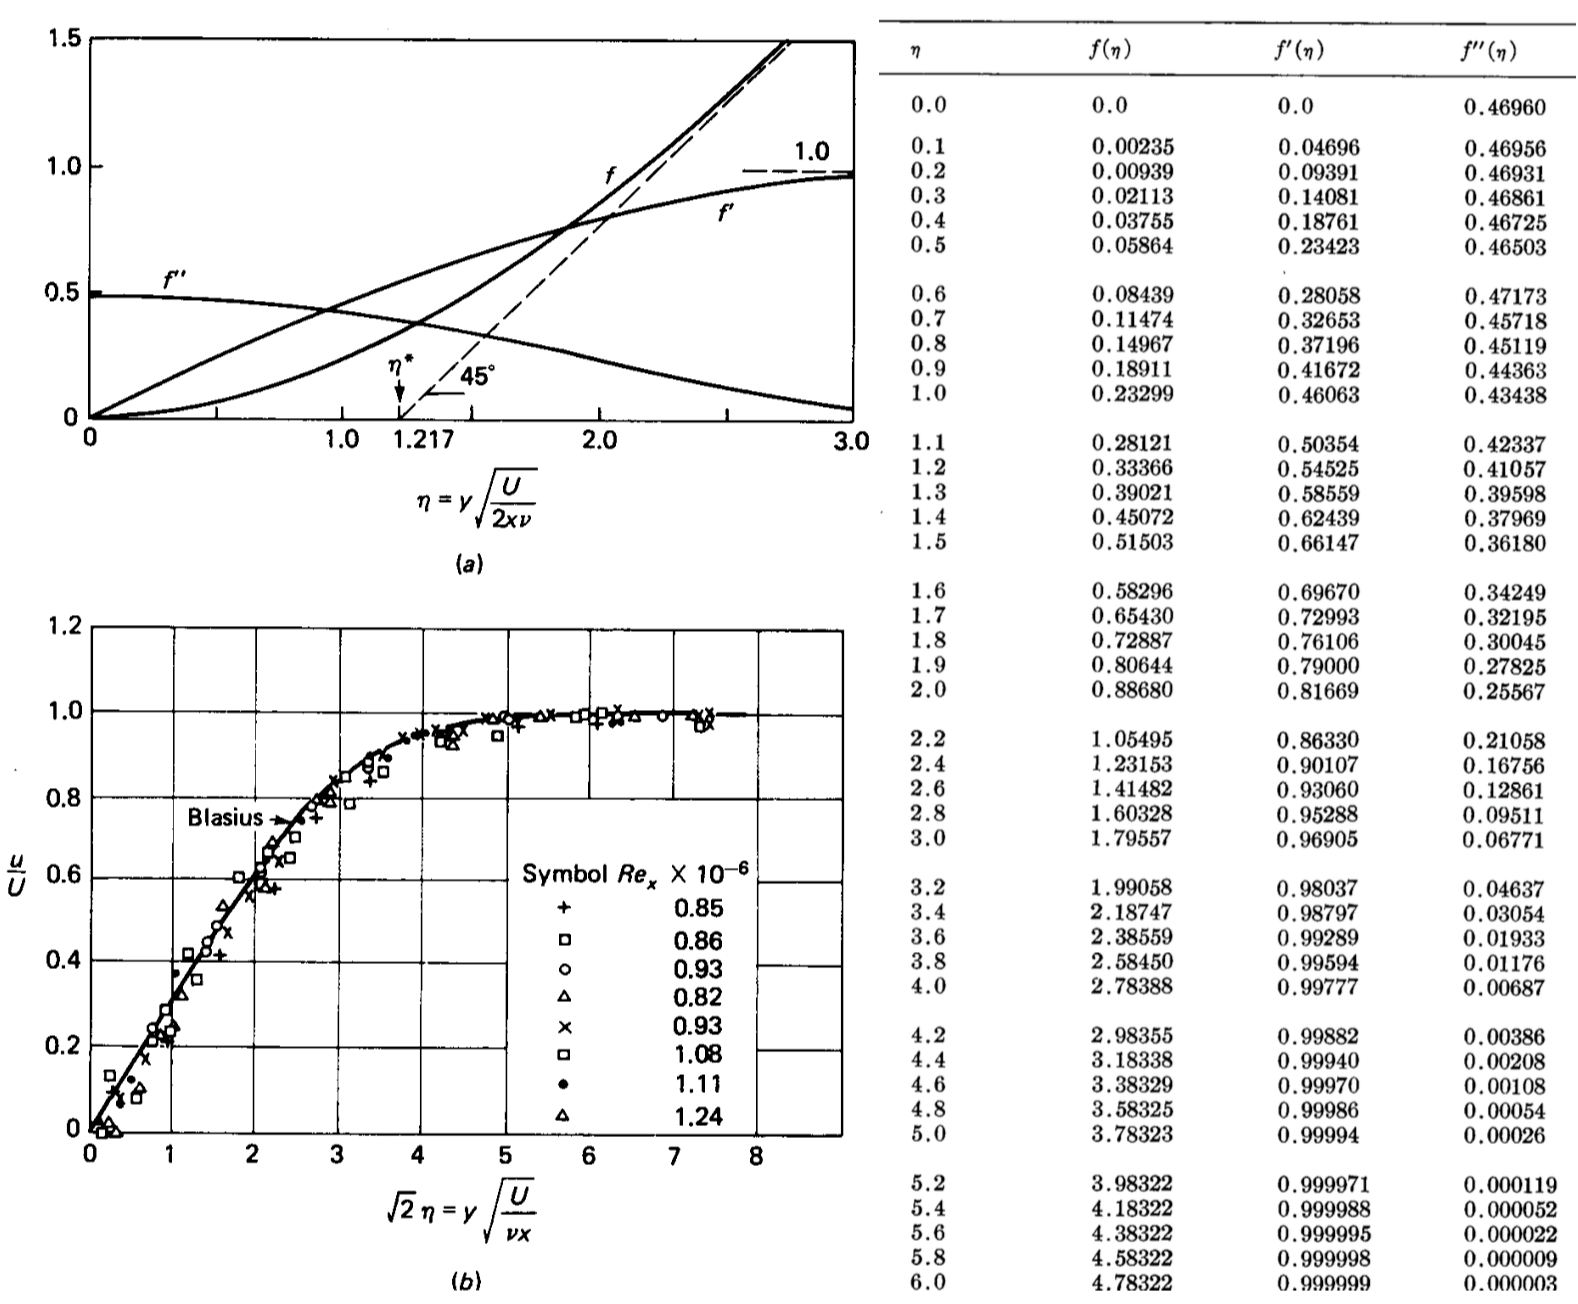
\includegraphics[scale=0.23]{ch5/7}
			\captionof{figure}{}	
			\label{fig:5.7}
			\end{wrapfigure}
			We fall on the same condition as the IC. This is fortunate because \eqref{eq:5.22} is a third order equation so it needs only 3 conditions. It remains to find $f$ by solving this equations with these conditions and that's what Blasius did. It looks simple but there isn't analytical solutions, he used expansion in series. The solutions are shown at the top on \autoref{fig:5.7} and at the bottom we find the experimental data giving the velocity profile for various value of $x$. We see that the data nicely collapse with the same curve. But why we determined the boundary layer? For friction! So let's exploite the results.
			
		\subsubsection{Exploitation of the results} 
			Let's remind the expression for friction 
			
			\begin{equation}
				\tau_w = \mu \left( \frac{\partial u}{\partial y}\right)_w  = \frac{\mu}{l} f''(0) \uinf = \sqrt{\frac{\uinf}{2\nu x}}\mu f''(0)\uinf
			\end{equation}
			
			In fluid mecanics we love dimensionless numbers so we use the \textbf{friction coefficient}
			
			\begin{equation}
				C_f = \frac{\tau _w}{\rho \uinf ^2 /2} = \frac{2 \uinf}{\rho \uinf ^2}\sqrt{\frac{\uinf}{2\nu x}} \mu f''(0) = \sqrt{\frac{2\nu}{\uinf x}} f''(0) = \frac{\sqrt{2}f''(0)}{\sqrt{Re_x}} = \frac{2 f''(0)}{Re_l}
			\end{equation}
			
			where the last equivalence comes from \eqref{eq:5.23}. Looking at the table, we find the last result 
			
			\begin{equation}
				C_f = \frac{0.664}{\sqrt{Re_x}}
			\end{equation}
			
			What's the physical interpretation of $l$.  We said it was some percentage velocity thickness. When $\eta = 1$, $f'(\eta) = 0.46$, so $l$ is the $46\%$ velocity $\Rightarrow u = 0.46 \uinf$. Now we want to construct more physically based boundary layer thicknesses. 
			
		\subsubsection{Other characteristic thicknesses}
			\paragraph{Conventional thickness} There is one called the \textbf{conventional thickness} $\delta$ or $\delta _{.99}$, beeing the thickness where velocity reaches 99\% of the outer velocity. So 
			\begin{equation}
				\eta _{\delta} =\frac{\delta _{.99}}{l(x)} \mbox{ is such that } f'(\eta _\delta) = 0.99. 
			\end{equation}
			
			Using the tables we find that it corresponds to 
			
			\begin{equation}
			\begin{aligned}
				&\eta _\delta = 3.5 \qquad \Rightarrow \delta _{.99} = 3.5 l(x) = 3.5 \sqrt{\frac{2\nu x}{\uinf}} \approx 5 \sqrt{\frac{\nu x}{\uinf}} \qquad \Leftrightarrow \frac{\delta _{.99}}{x} = \frac{5}{\sqrt{Re_x}}\\
				&\Rightarrow Re_\delta = 5 Re_x
			\end{aligned}			
			\end{equation}
			
			\begin{wrapfigure}[9]{l}{4cm}
			\vspace{0mm}
			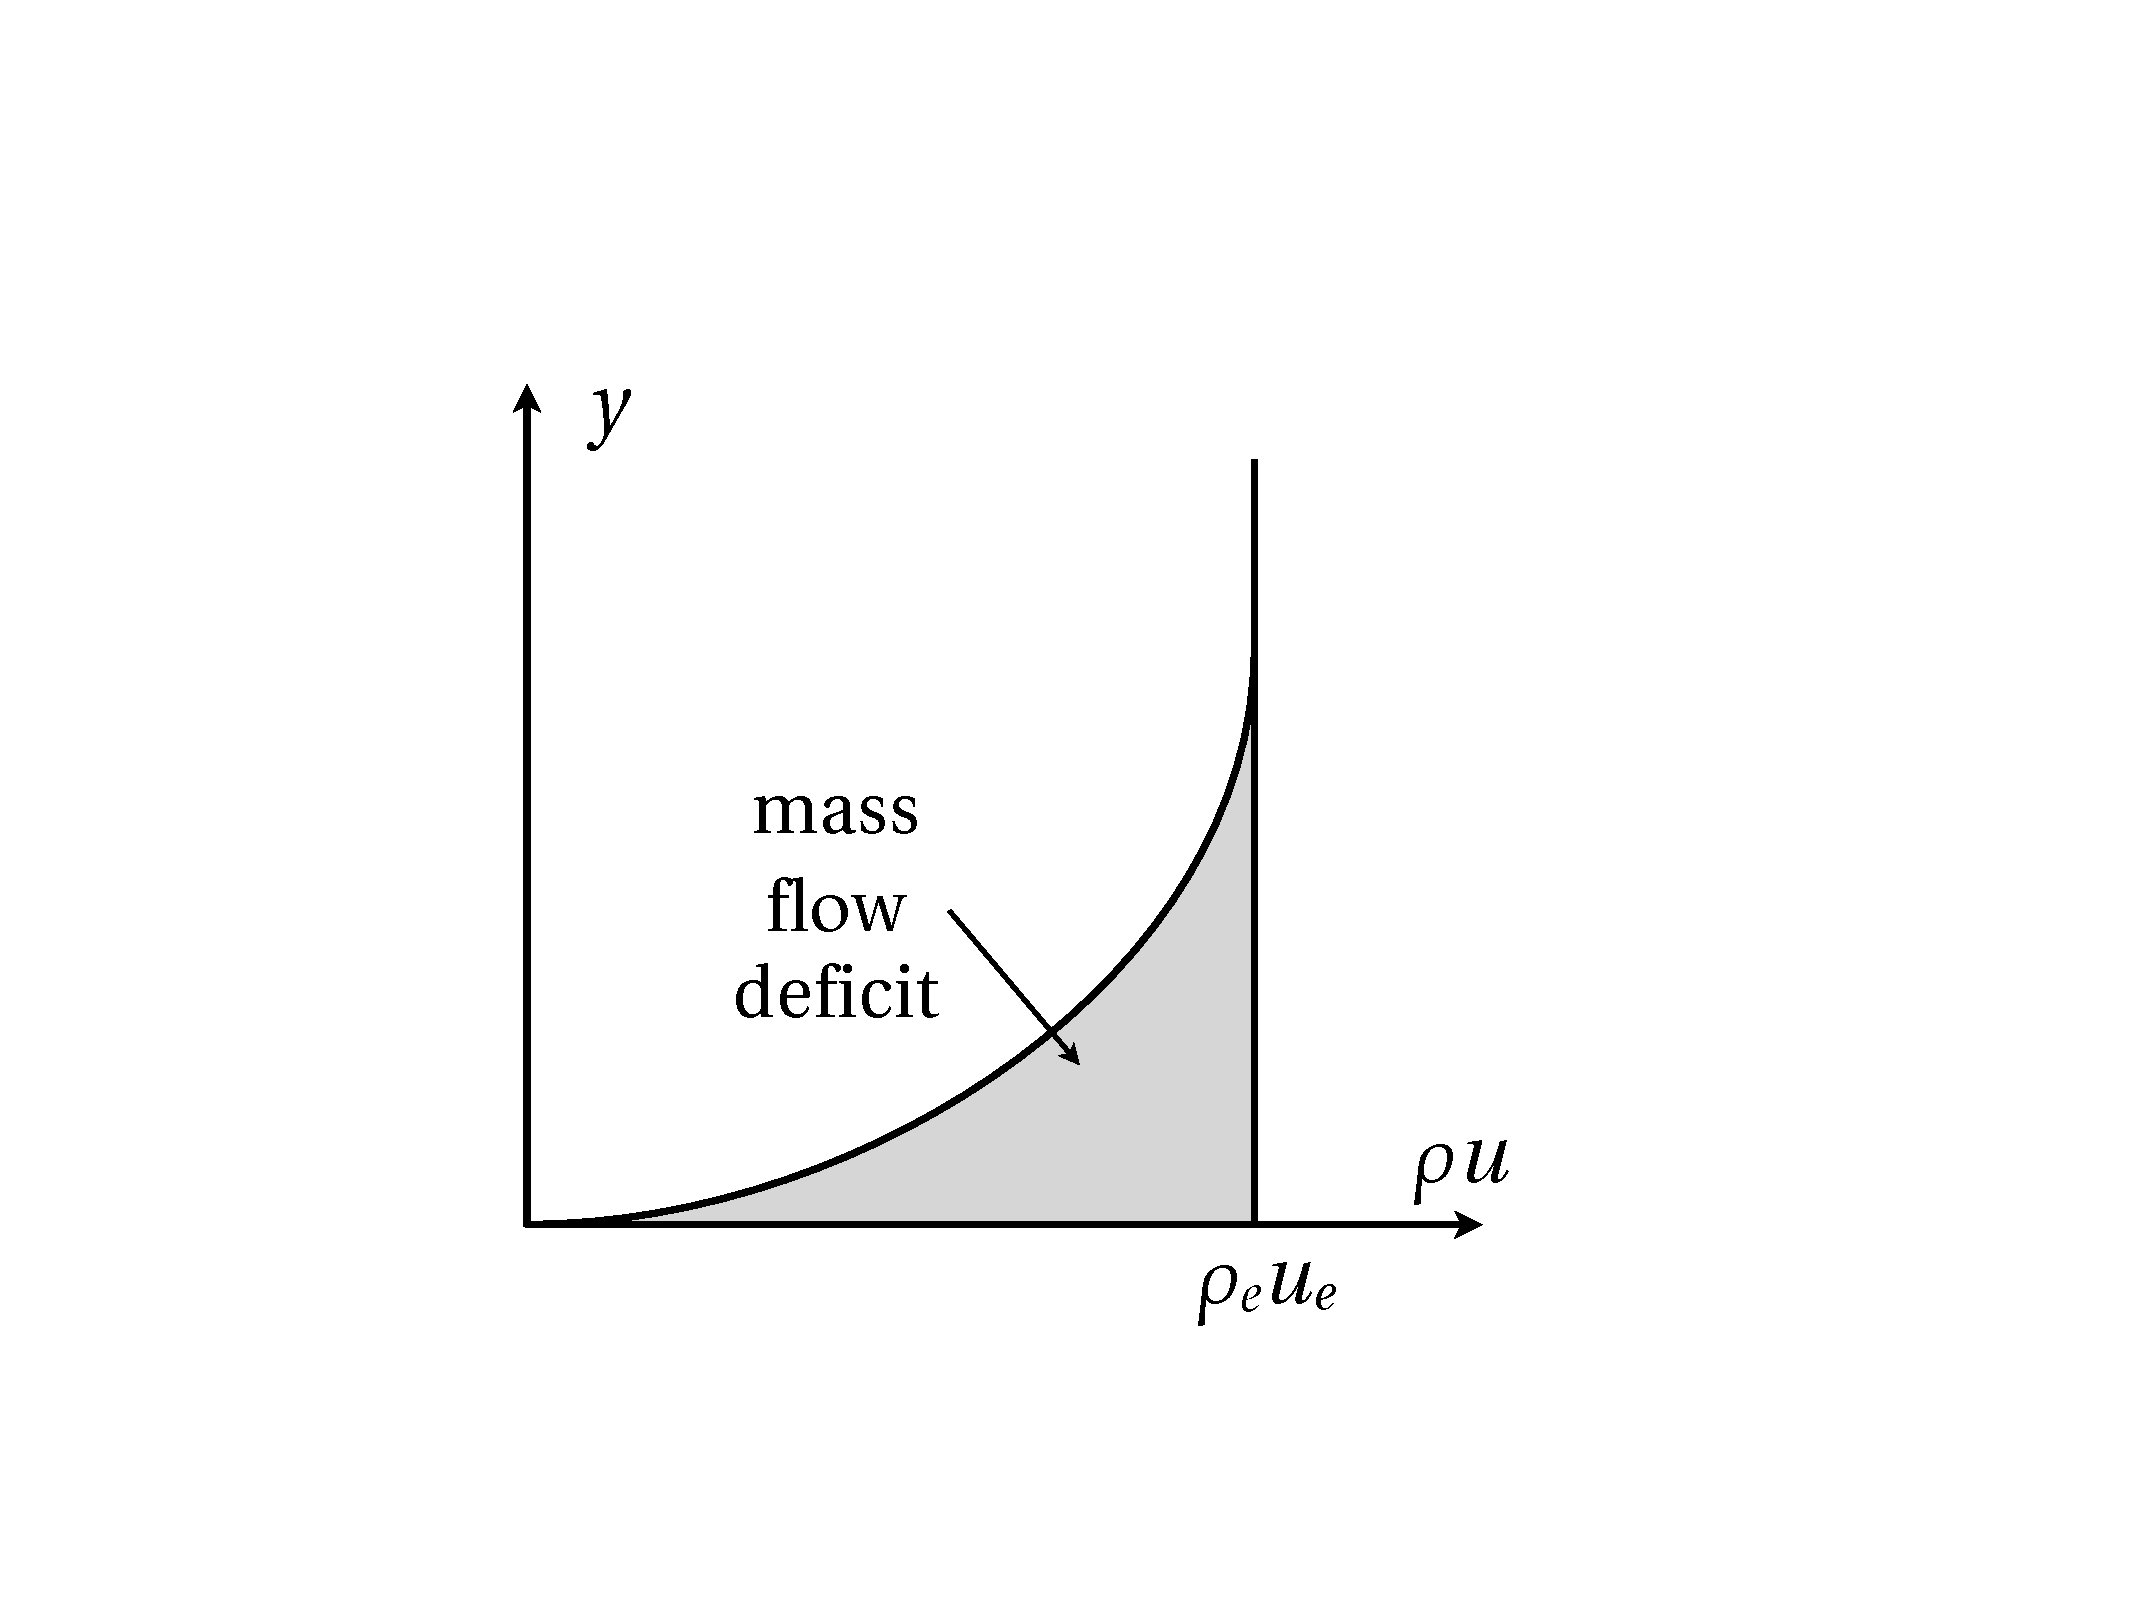
\includegraphics[scale=0.23]{ch5/8}
			\captionof{figure}{}	
			\label{fig:5.8}
			\end{wrapfigure}
			This is necessary because if we take the table and try to identify $\delta _{.99}$, the angle is not accurate. This is no more physical than the 46\% thickness. 
			
			\paragraph{Mass flow defect thickness} Something more physical is found when we replot $\rho u$ in function of $y$ and compare it to the inviscid vertical profile $u = \uinf$. When we integrate the mass flow near the wall, there is a mass flow defecit and a thickness based on which are
			
			\begin{equation}
			\begin{array}{c}
				\mbox{Mass flow deficit} = \rho \int _0 ^\infty (\uinf - u)\, dy \\
				\mbox{Mass flow defect thickness}:\\
				 \delta ^* = \frac{\rho \int _0 ^\infty (\uinf - u) dy }{\rho \uinf} = \int _0 ^\infty \left( 1-\frac{u}{\uinf} \right)\, dy
			\end{array}
			\end{equation}
			
			The value for the flate plate/zero pressure gradient is 
			
			\begin{equation}
				\delta ^* = \int _0^\infty (1- f') l\, dy = l\underbrace{\int _0^\infty (1-f') \, dy}_{\eta ^*}\qquad \Rightarrow Re_{\delta ^*} = Re_{l}\eta ^* = \sqrt{2Re_x}\eta ^* .
			\end{equation}
			
			\begin{wrapfigure}[6]{r}{6.5cm}
			\vspace{-5mm}
			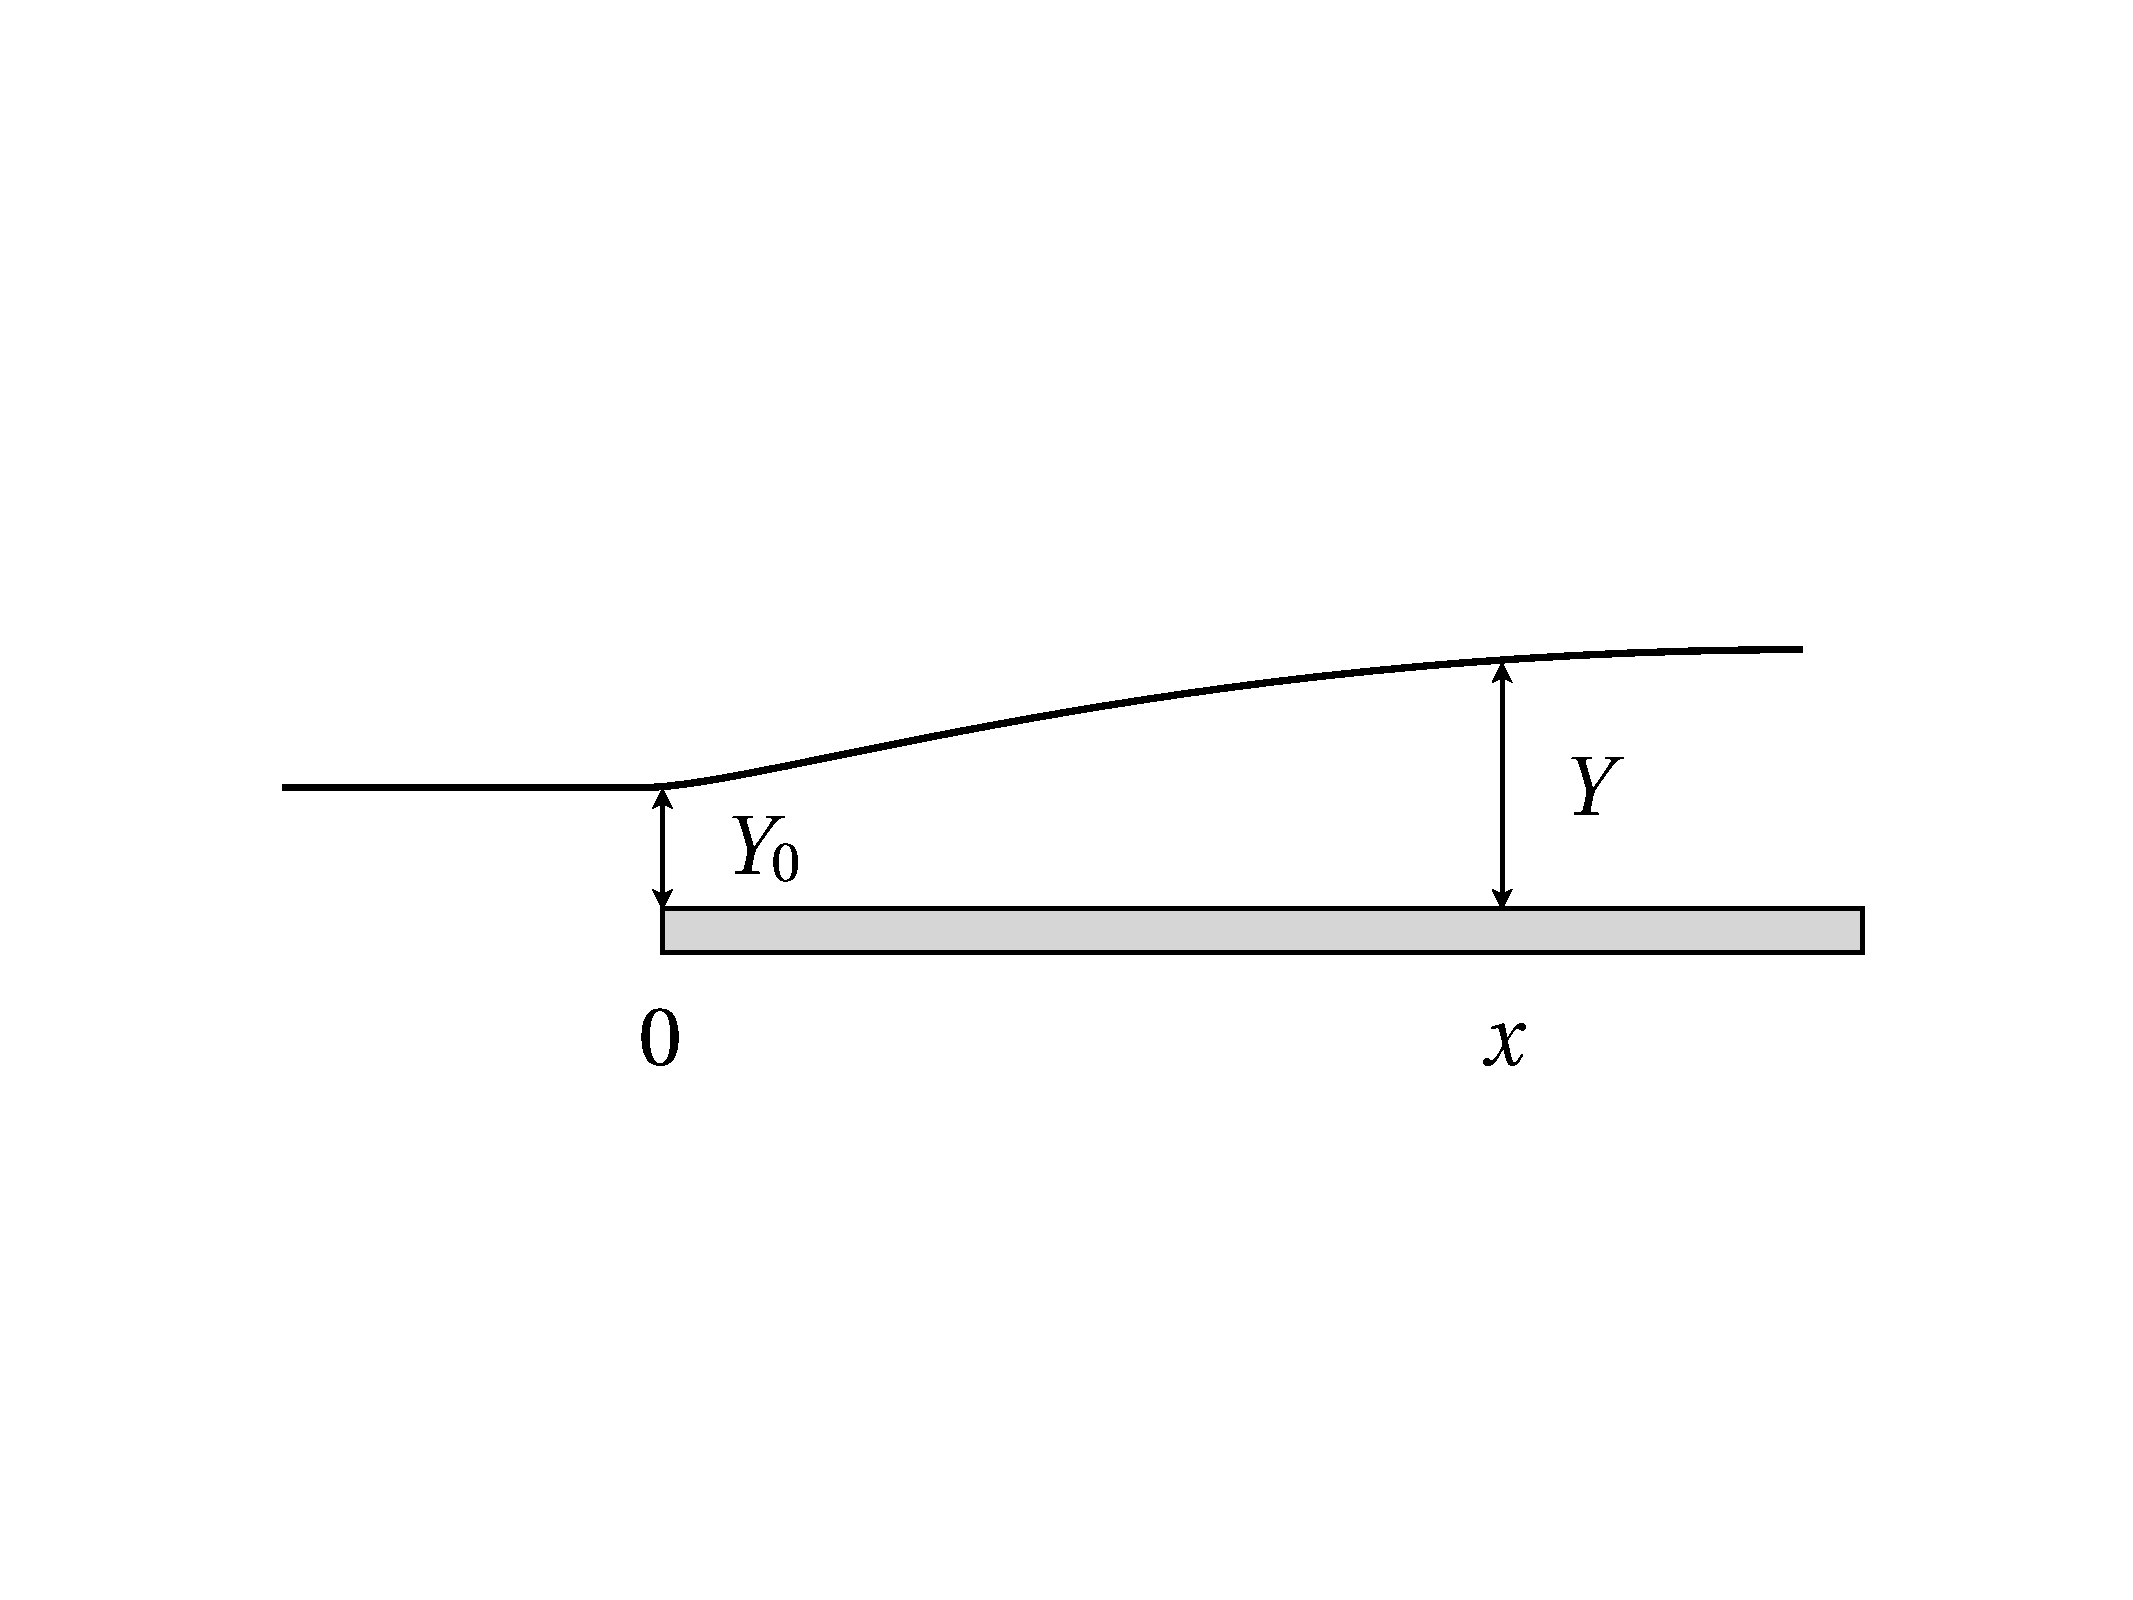
\includegraphics[scale=0.23]{ch5/9}
			\captionof{figure}{}	
			\label{fig:5.9}
			\end{wrapfigure}
			Let's now give a physical meaning to that mass flow deficit. Let's consider the infinitely thick flat plate and a streamline in the outer region flow which is deviated because of the presence of the boundary layer $y(x) \neq y_0$. Mass conservation tells us that 
			
			\begin{equation}
			\begin{aligned}
				&\rho \int _0^{y_0} u_\infty \, dy =  \rho \int _0^y u(x,y) \, dy \qquad \Leftrightarrow \rho \int _0^{y} u_\infty \, dy - \rho \int _{y_0}^{y} u_\infty \, dy = \rho \int _0^y u(x,y)\infty \, dy \\
				\Leftrightarrow \ &\rho \int _0^{y} (u_\infty - u) \, dy = \rho \int _{y_0}^{y} u_\infty \, dy \qquad \Leftrightarrow y-y_0 = \int _0^{y} \left(1 -\frac{u}{\uinf}\right)\, dy = \delta ^*
			\end{aligned}
			\end{equation}
			
			We see that the deviation of the streamline is exactly $\delta ^*$ called the \textbf{displacement thickness}. One last thing to draw attention, we saw that $f'  \rightarrow 1 \Rightarrow f = \eta + C$. This constant is 
			
			\begin{equation}
				C = \lim _{\eta \rightarrow \infty}  (f-\eta ) = \lim _{\eta \rightarrow \infty}  \int _0 ^\eta (f'-1) \, d\eta = \int _0^\infty (f'-1)\, d\eta = -\eta ^*.
			\end{equation}
			
			We can see this on the table graph where if we extrapolate to the x axis we find $\eta ^*$. We have imposed the matching condition to the tengential velocity profile. What's the asymptotic value of the normal velocity? It is the limiting value of $F = \eta f' - f$ 
			
			\begin{equation}
				\lim _{y \rightarrow \infty} v = \uinf \frac{dl}{dx}\eta ^*\neq 0.
			\end{equation}
			
			There we have normal velocity mismatch. This is due to the consideration we made at the beginning saying that streamlines were straight but now we conclude that they are not straight. We do not take into account the perturbation of the outer inviscid flow induced by the presence of the viscous layer. 
			
			\begin{wrapfigure}[11]{l}{4cm}
			\vspace{0mm}
			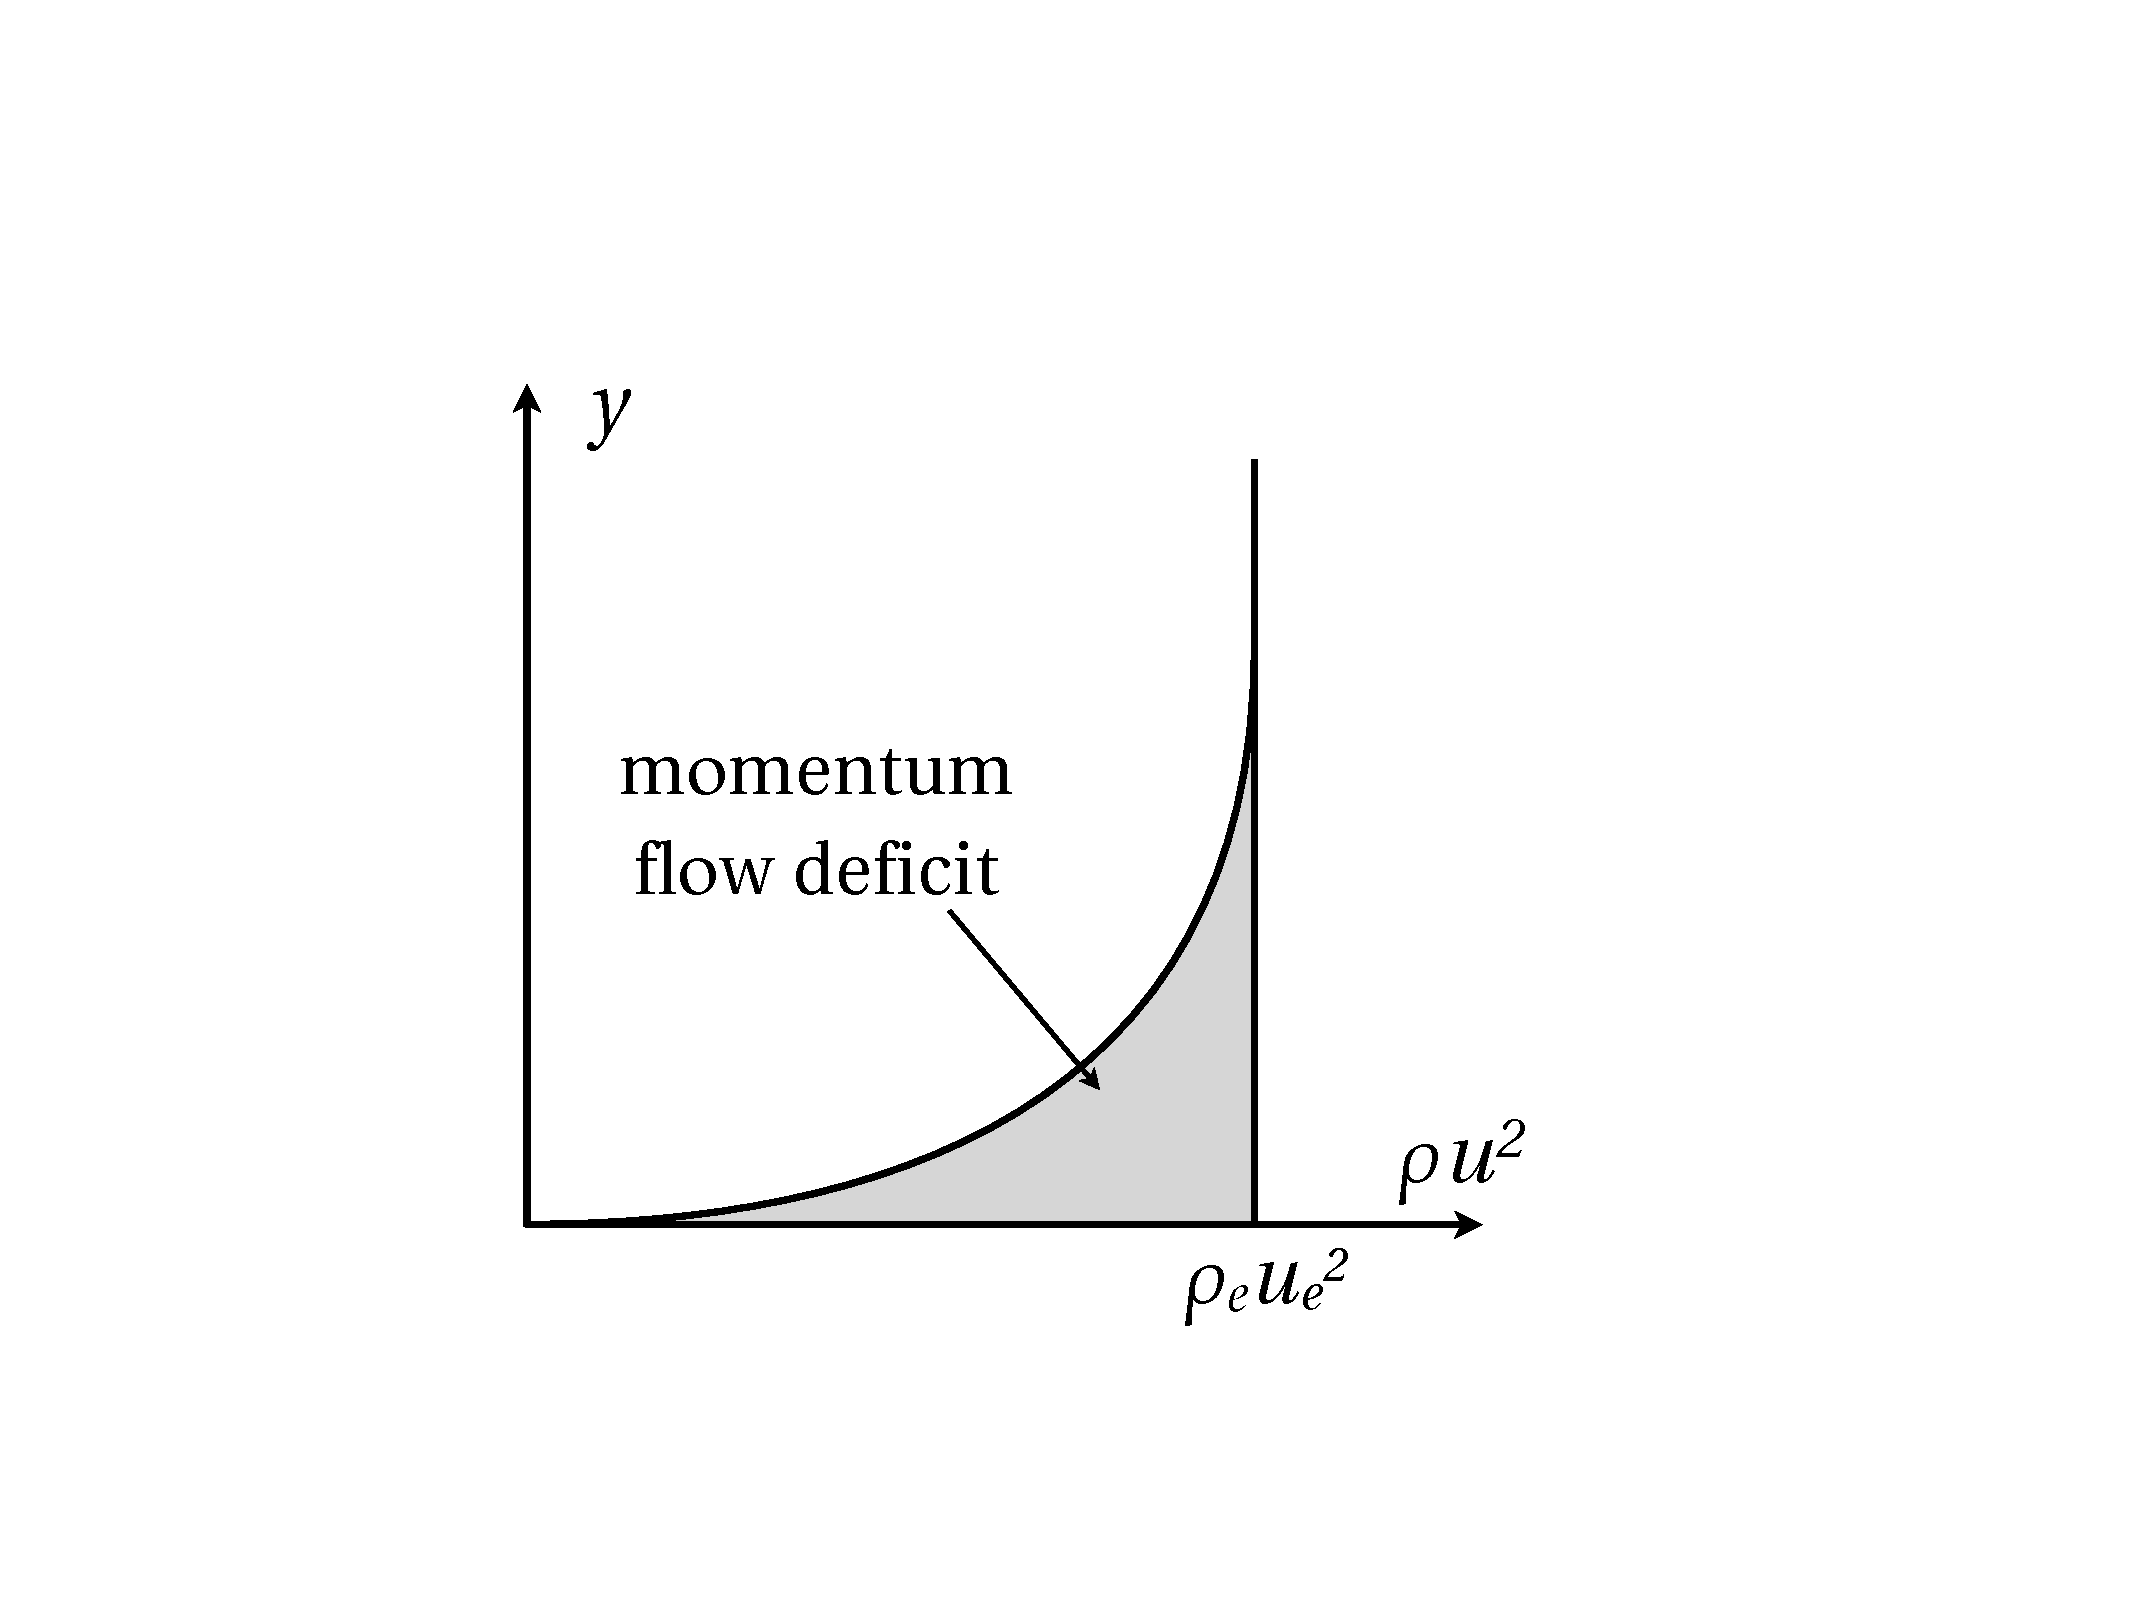
\includegraphics[scale=0.23]{ch5/10}
			\captionof{figure}{}	
			\label{fig:5.10}
			\end{wrapfigure}
			\paragraph{Momentum flow defect thickness}
			Similarly to the mass flow defect, we can define the momentum flow defect as beeing 
			
			\begin{equation}
				\mbox{MoFD} = \int_0^\infty \rho \left(  \uinf ^2 - u^2 \right) \, dy
			\end{equation}
		
			If we draw attention to to the math definition of the previous $\delta ^*$, we notice that it is the hight in the plot of the rectangle that have the same area as the one formed by the curve. We can define a momentum induced by the mass flow by multiplying its expression by $\uinf$ and by defining the \textbf{extra momentum flow defect} and the corresponding \textbf{momentum flow defect thickness}
			
			\begin{equation}
			\begin{aligned}
				&\mbox{XMoFD} =  \int_0^\infty \rho \left(  \uinf ^2 - u^2 \right) \, dy - \uinf \int_0^\infty \rho \left( \uinf -u \right)\, dy 
= \int_0^\infty \rho u \left(\uinf - u\right) \,  dy\\
				&\mbox{MoFDT} = \frac{\mbox{XMoFD}}{\rho \uinf ^2} = \theta = \int_0^\infty \frac{ u}{\uinf} \left( 1 - \frac{u}{\uinf} \right)\, dy
			\end{aligned}
			\end{equation}
			
			For the case of the flat plate, we know $\frac{u}{\uinf} = f'$, so
			
			\begin{equation}
				\theta = l \underbrace{\int _0^\infty f' (1-f') \, d\eta}_{\theta ^*} = l\theta ^* = \frac{\sqrt{2}x}{\sqrt{Re_x}} \theta ^*.
			\end{equation}
			
			To find the value of $\theta ^*$, we can integrate by part we find
			
			\begin{equation}
			\begin{aligned}
				\theta ^* &= \int _0^\infty (1-f') \underbrace{f' \, d\eta}_{df} = \underbrace{\left[ f (1-f') \right]_0^\infty}_{=0} + \int_0^\infty f f'' \ d\eta\\
				\eqref{eq:5.22} \Rightarrow &= \int_0^\infty - f''' \, dy = f''(0) = 0.664.
			\end{aligned}
			\end{equation}
			
			This conclues this section but keep in mind that we have a normal velocity mismatch. However, in \eqref{eq:5.20} appears $\frac{fl}{dx}$ which is equal by \eqref{eq:5.22} to 
			
			\begin{equation}
				\frac{dl}{dx} = \frac{1}{Re_l}\qquad =0 \ for \ Re_l \rightarrow \infty
			\end{equation}
			
			So we see that the mismatch disappear for Re number going to $\infty$. This means that classical boundary theory is valid only in the case of infinite Re number, for a finite Re there is a finite mismatch. 
			
			
\section{Other pressure gradient}
	The equations and initial conditions are the same except for the pressure term
	
	\begin{equation}
		\begin{aligned}
		&\frac{\D u}{\D x} + \frac{\D v}{\D y} = 0\\
		&u \frac{\D u}{\D x} + v \frac{\D u}{\D y} =- \frac{1}{\rho} \frac{dp_e}{dx}+ \nu \frac{\D ^2 u}{\D y^2}
	\end{aligned}	
	\label{eq:5.44}
	\end{equation}
	
	Because of the variation of the tangential pressure, there is a variation of the tangential velocity. Indeed, if we take the momentum equation for the inviscid flow we have 
	
	\begin{equation}
		u \frac{\D u}{\D x} =- \frac{1}{\rho} \frac{dp_e}{dx}
	\end{equation}
	
	which means that the outer velocity is not constant if the outer pressure is not constant. In other words, for a position $x_1$ we will have a $u_{e_1}$ different of the velocity $u_{e_2}$ of a position $x_2$. We also see that a positive pressure gradient corresponds to a decelarating flow due to the minus sign and vice-versa. We can now wonder if there is also a self-similar solution. 
	
	\begin{center}
	\begin{minipage}{0.49\textwidth}
\begin{center}
	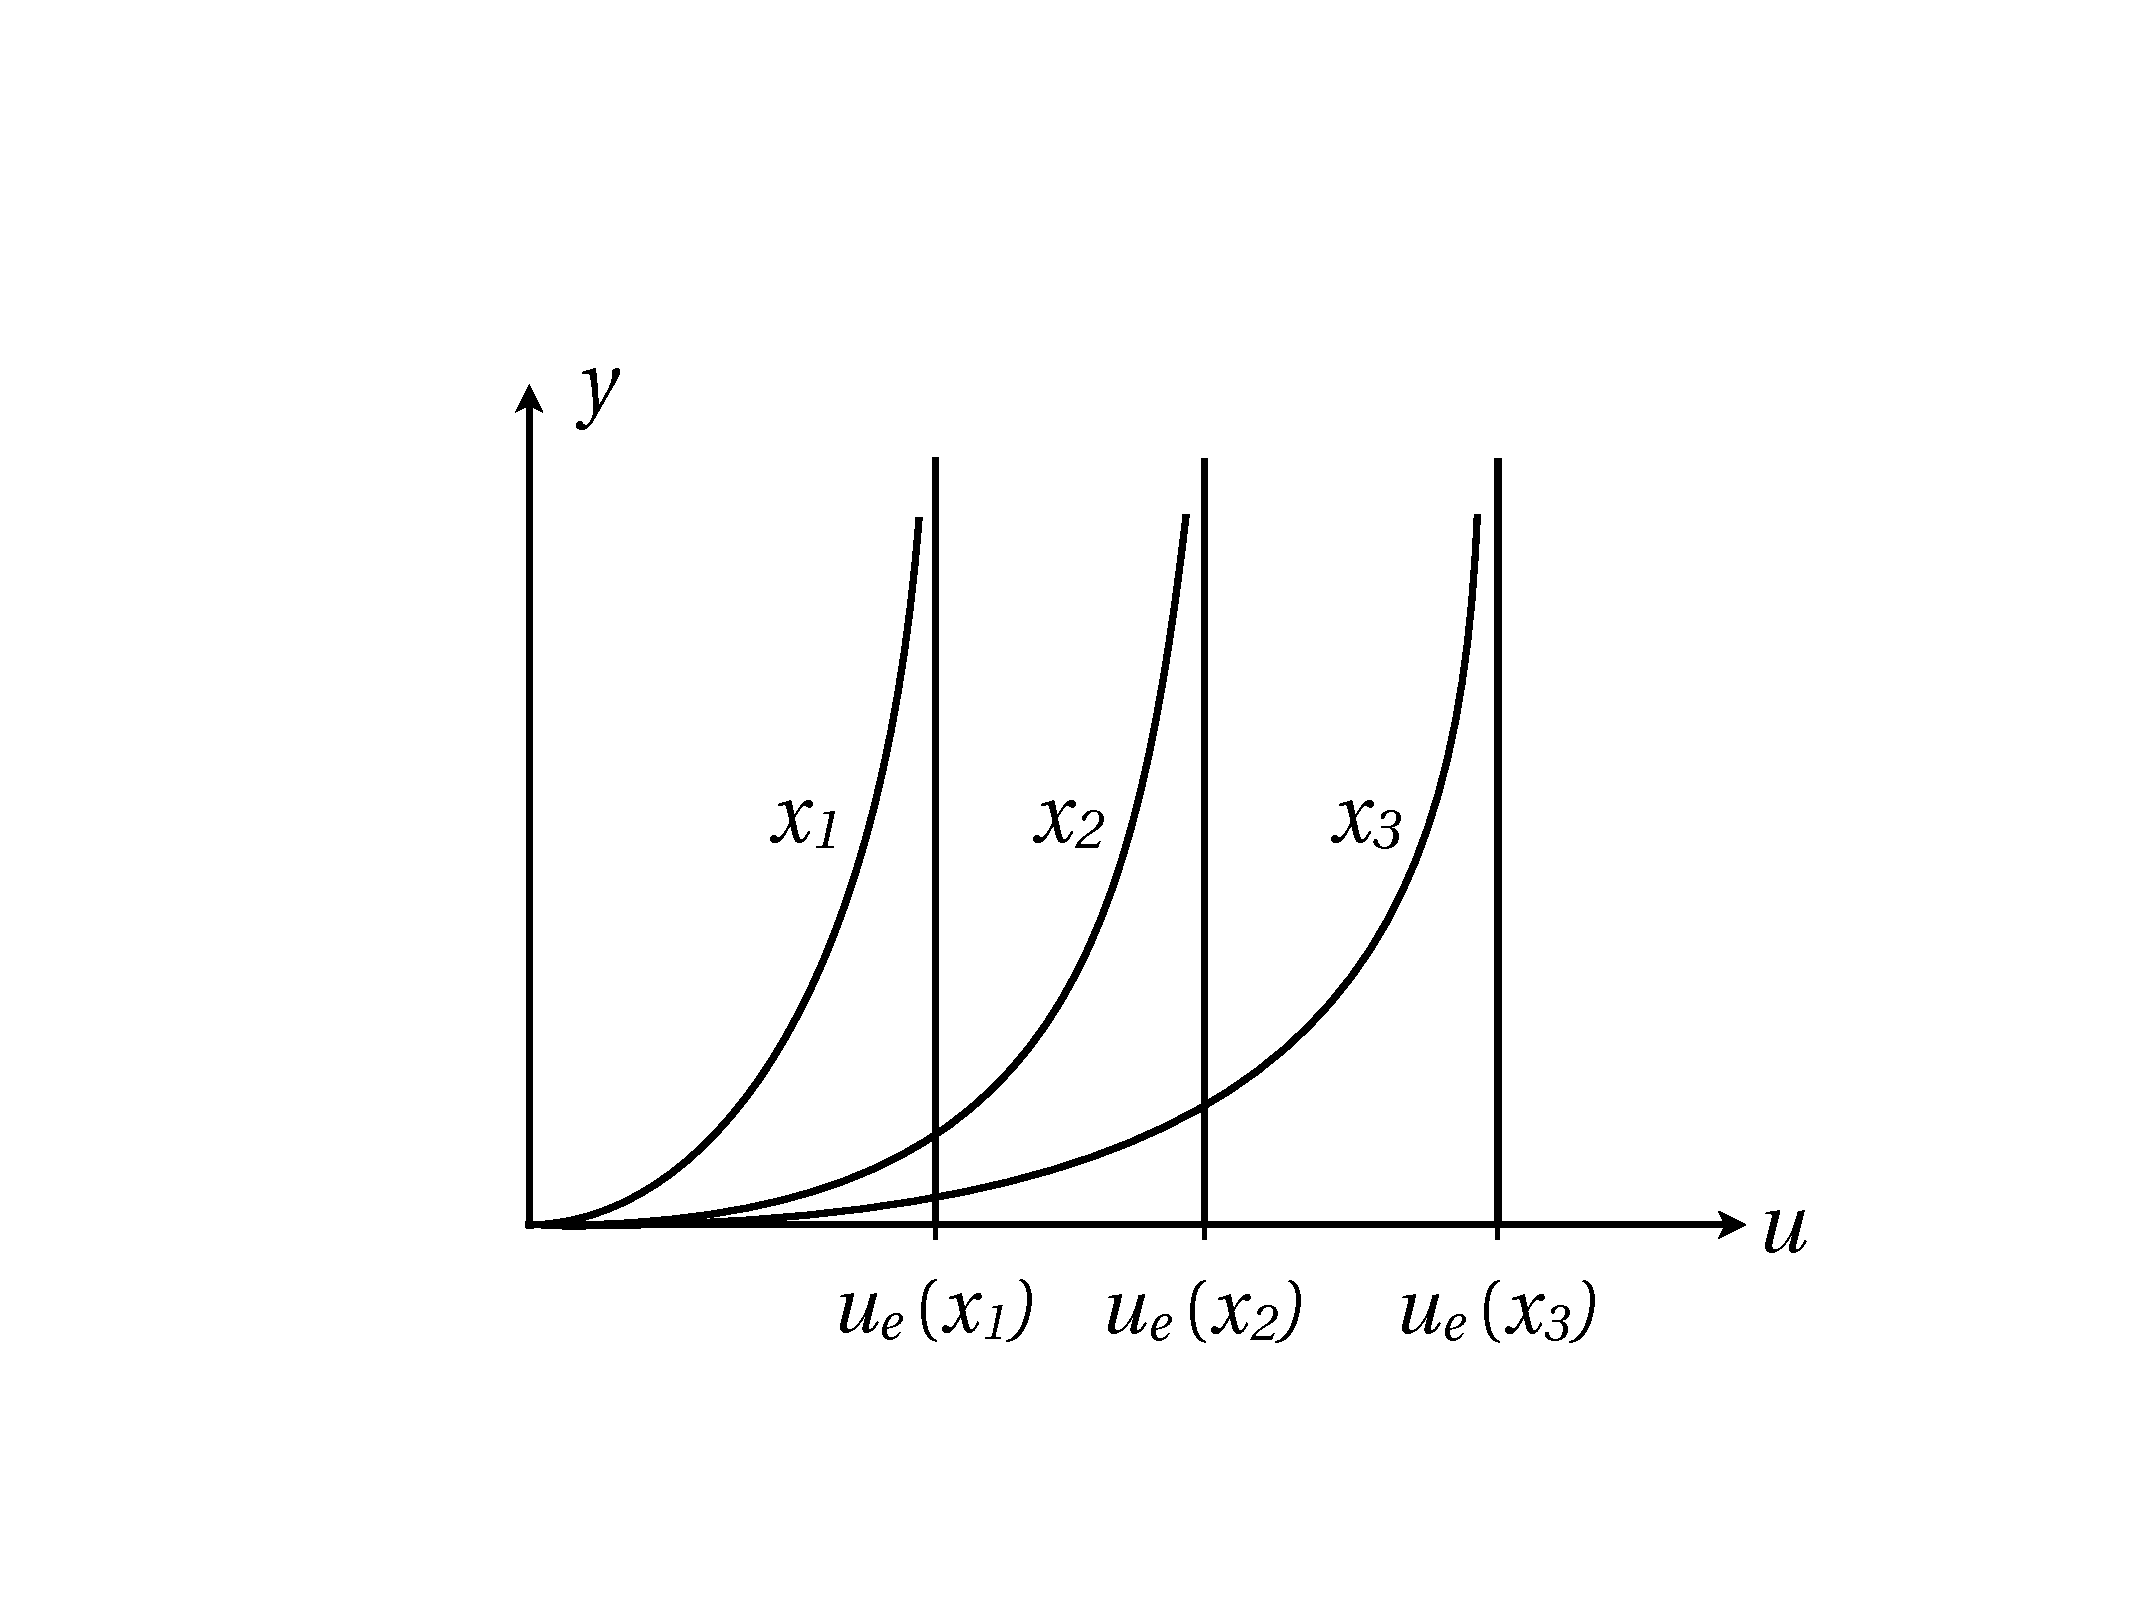
\includegraphics[scale=0.25]{ch5/11}
	\captionof{figure}{}
\end{center}
	\label{fig:5.11}
	\end{minipage}
	\begin{minipage}{0.49\textwidth}
\begin{center}
	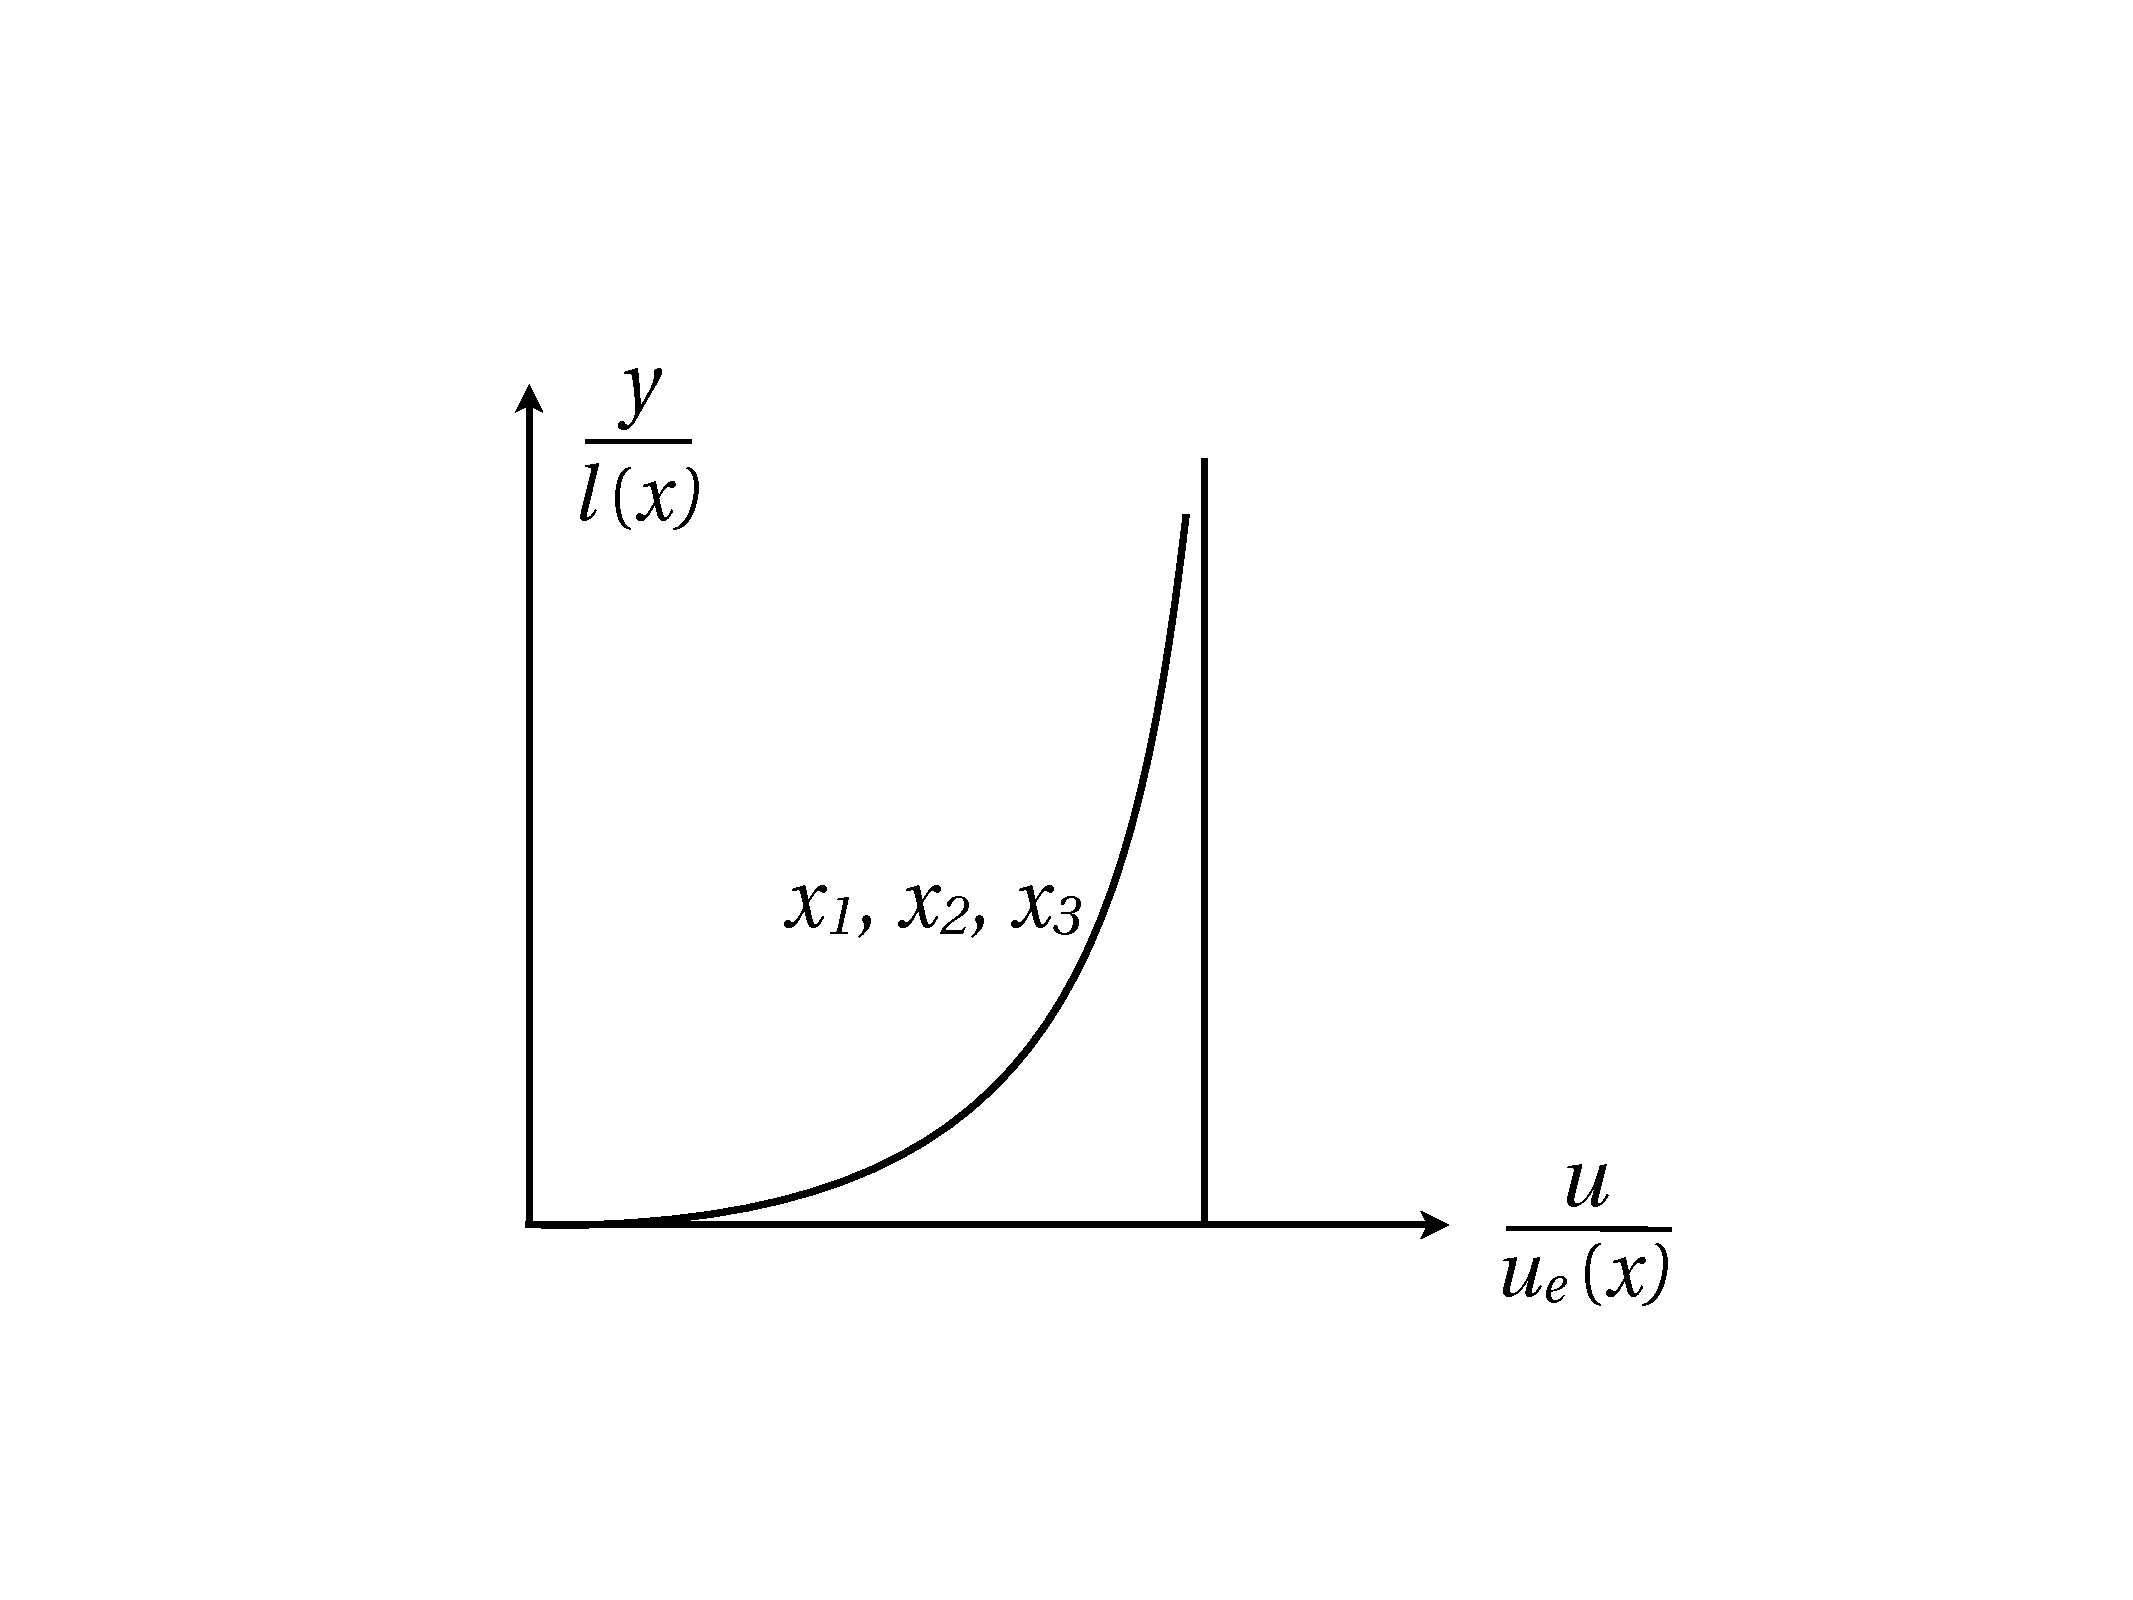
\includegraphics[scale=0.25]{ch5/12}	
	\captionof{figure}{}
\end{center}
	\label{fig:5.12}
	\end{minipage}
	\end{center}
	
	If we replot y in funtion of u, we will have a different plot compared to the flat plate because of the changing value of $u_{e_x}$ as shown on \autoref{fig:5.11}. So to make these velocity profiles collapse in a single one we need to scale the velocity and y and not only y as previously. So if we plot $\frac{y}{l(x)}$ in function of $\frac{u}{u_e(x)}$, we must have a single velocity profile with an asymptote at 1, whatever the value of x as shown on \autoref{fig:5.12}. Again we don't know we will have to check. There is a difference between the two plot axis, $l(x)$ is unknown but $u_e(x)$ is known by the calculation on the outer flow. For the same coordinate transformation \eqref{eq:5.14}
	
	\begin{equation}
		\frac{u}{u_e(x)} = g(\cancel{\xi}, \eta)  \qquad \Leftrightarrow u = u_e(x)
	\end{equation}
	
	That's the \textbf{self-similarity assumption}. \eqref{eq:5.17} is therefore valid to the condition of replacing $\uinf$ by $u_e(x)$
	
	\begin{equation}
		\begin{aligned}
			&\frac{\D u}{\D x} = \frac{du_e}{dx}g(\eta ) + u_e\underbrace{\frac{\D g}{\D \eta}}_{u_e(x) g'} \underbrace{\frac{\D \eta}{\D x}}_{-\frac{y}{l^2(x)}\frac{dl}{dx}} = \frac{du_e}{dx}g(\eta )  - u_e(x) g'(\eta)\eta \frac{1}{l(\xi)} \frac{dl(\xi)}{d\xi}\\
			&\frac{\D u}{\D y} = u_e(x)\frac{\D  g}{\D \eta} \frac{1}{l(\xi)} = u_e(x) \frac{g'}{l(\xi)} \qquad and \qquad \frac{\D ^2 u}{\D y }= u_e(x) \frac{g''}{l^2(\xi)}
		\end{aligned}
		\end{equation}
		
		\subsubsection{Continuity equation}
			The process is exactly the same as last time except that we will have the additional term due to $\frac{\D u}{\D x}$ 
			
			\begin{equation}
			\begin{aligned}
				&\frac{\D v}{\D y} = -\frac{\D u}{\D x} = -\frac{du_e}{dx}g(\eta )  + u_e g'\frac{\eta}{l} \frac{dl}{d\xi} \\
				&v(x,y) = -\frac{du_e}{dx} l \int _0 ^\eta \underbrace{g(\zeta) \, d\zeta }_{f}+ u_e \frac{dl}{d\xi} \underbrace{\int _0 ^\eta \zeta g'(\zeta) \, d\zeta}_{F= \eta f' -f} \\
				&v = -l \frac{du_e}{dx} f + u_e \frac{dl}{dx} (\eta f' - f)
			\end{aligned}
			\end{equation}
			
			which is the same expression with an additional term. 
			
		\subsubsection{Momentum equation}
			Knowing that $u = u_e f'$, the momentum equation becomes
				
			\begin{equation}
			\begin{aligned}
				&u_ef' \left[ \frac{du_e}{dx}f' \cancel{- u_e f''\frac{\eta}{l}\frac{dl}{dx}} \right] + \left[-l \frac{du_e}{dx} f + u_e \frac{dl}{dx} (\cancel{\eta f'} - f)\right] u_e \frac{f''}{l} = u_e\frac{du_e}{dx} + \nu u_e \frac{f'''}{l^2}\\
				\Leftrightarrow \qquad &\underbrace{\frac{\nu u_e }{l^2}}_{F_1(x)}f''' + \underbrace{u_e \frac{du_e}{dx}}_{F_2(x)} \left[1 - {f'}^2 + ff'' \right] + \underbrace{ \frac{u_e^2}{l}\frac{dl}{dx}}_{F_3(x)}ff'' = 0 \\
				\Leftrightarrow \qquad &\frac{F_1(x)}{F_3(x)}f''' + \frac{F_2(x)}{F_3(x)}(1-f'^2+ff'') + ff''=0 
			\end{aligned}
			\label{eq:5.49}
			\end{equation}
			
			For this last equation to admit a solution, it must be reductible to a simple function of $\eta$. This implies that \textbf{the self similarity conditions} are
			
			\begin{equation}
				\frac{F_1(x)}{F_3(x)} = cst  =\frac{F_3(x)}{F_1(x)} \qquad and \qquad \frac{F_2(x)}{F_3(x)} = cst = \frac{F_3(x)}{F_2(x)}
			\end{equation}
			
			Let's write completely $\frac{F_2(x)}{F_3(x)}$ and $\frac{F_3(x)}{F_1(x)}$
			
			\begin{equation}
			\begin{aligned}
				&\frac{F_2(x)}{F_3(x)} =  \frac{\frac{du_e}{u_e dx}}{\frac{dl}{ldx}} = \frac{\frac{d\ln u_e}{dx}}{\frac{d \ln l}{dx}} = k \qquad \Leftrightarrow \ln u_e =k \ln l + c \qquad \Leftrightarrow u_e = K l ^k\\
				&\frac{F_3(x)}{F_1(x)} = u_e\frac{dl}{dx} \frac{l}{\nu } = \frac{K}{\nu}l^{k+1}\frac{dl}{dx} = \frac{K}{\nu (k+2)} \frac{dl^{k+2}}{dx} = cst \qquad \Leftrightarrow \left\{\begin{aligned} l &\propto x^{\frac{1}{k+2}}\\
				u_e &\propto x^{\frac{k}{k+2}} \end{aligned}\right.
			\end{aligned}
			\end{equation}
			
			The conclusion is that we will have a solution if the velocity distribution is a power of x 
			
			\begin{center}
			\theor{			
			\begin{equation}
				u_e = ax^m \qquad and \qquad \frac{du_e}{dx} = amx^{m-1} = m\frac{u_e}{x}
			\end{equation}
			}
			\end{center}
			
			Now we can look at $\frac{F_2(x)}{F_1(x)}$ to see what happens
			
			\begin{equation}
				\frac{F_2(x)}{F_1(x)} = \frac{u_e \frac{du_e}{dx}}{\frac{\nu u_e}{l^2}} = cst \qquad \Leftrightarrow l^2 \propto \frac{1}{\frac{du_e}{dx}} \propto \frac{x}{u_e} \qquad \Leftrightarrow l \propto \sqrt{\frac{bx}{u_e}}
			\end{equation}
			
			where $b$ is an arbitrary constant to specify that $l$ is defined up to an arbitrary constant. Let's now compute the coefficients $F_1, F_2, F_3$ 
			
			\begin{equation}
				\frac{\nu u_e }{l^2} = \frac{\nu u_e^2}{bx} \qquad u_e \frac{du_e}{dx} = m\frac{u_e^2}{x} \qquad \frac{u_e^2}{l}\frac{dl}{dx} = u_e^2\frac{d\ln l}{dx} = \frac{u^2}{2} \left( \frac{1}{x} - \frac{m}{x} \right)
			\end{equation}
			
			After simplifying $\frac{u_e^2}{x}$ and replacing in \eqref{eq:5.49}, we have 
			\begin{equation}
				\frac{\nu}{b} f''' + m \left[1 - f'^2 + ff'' \right] + \frac{1}{2} ( 1 - m ) ff'' = 0 = f''' + ff'' \underbrace{\frac{1+m}{2} \frac{b}{\nu}} - f'^2 + \frac{mb}{\nu} (1-f'^2) 
			\end{equation}
			
			$b$ being an arbitrary constant, we will choose it such that we obtain the equation in the case of the flat plate with $\frac{1+m}{2} \frac{b}{\nu} = 1$ which is the 
			
			\begin{center}
			\theor{
			\textbf{Falkner-skan equation}
			\begin{equation}
				b = \frac{2\nu}{1+m} \qquad \Rightarrow f''' + ff'' + \underbrace{\frac{2m}{1+m}}_{\beta} (1-f'^2) = 0
			\end{equation}
			}
			\end{center}
			
			At this stage, let's notice that when: 
			\begin{itemize}
				\item[•] $m>0$: accelerating flow $\Rightarrow \beta > 0$.
				\item[•] $m<0$: decelerating flow $\Rightarrow \beta < 0$.
			\end{itemize}
			
			where $\beta$ can be seen as an acceleration parameter. We can see it easely by seeing that 
			
			\begin{equation}
				\frac{du_e}{dx} = m\frac{u_e}{x} \qquad \Rightarrow l^2 \frac{du_e}{dx} = m \frac{bx}{u_e}\frac{u_e}{x} = \frac{2 m\nu}{1+m} = \beta \nu \qquad \Rightarrow \beta = \frac{l^2}{\nu} \frac{du_e}{dx}
			\end{equation}
			
			where $\beta$ is really related to the velocity gradient. So when the velocity profile is a power of $x$, the self similar solution exist and its shape depends on $\beta$. 
			
\begin{center}
	\begin{minipage}{0.49\textwidth}
\begin{center}
	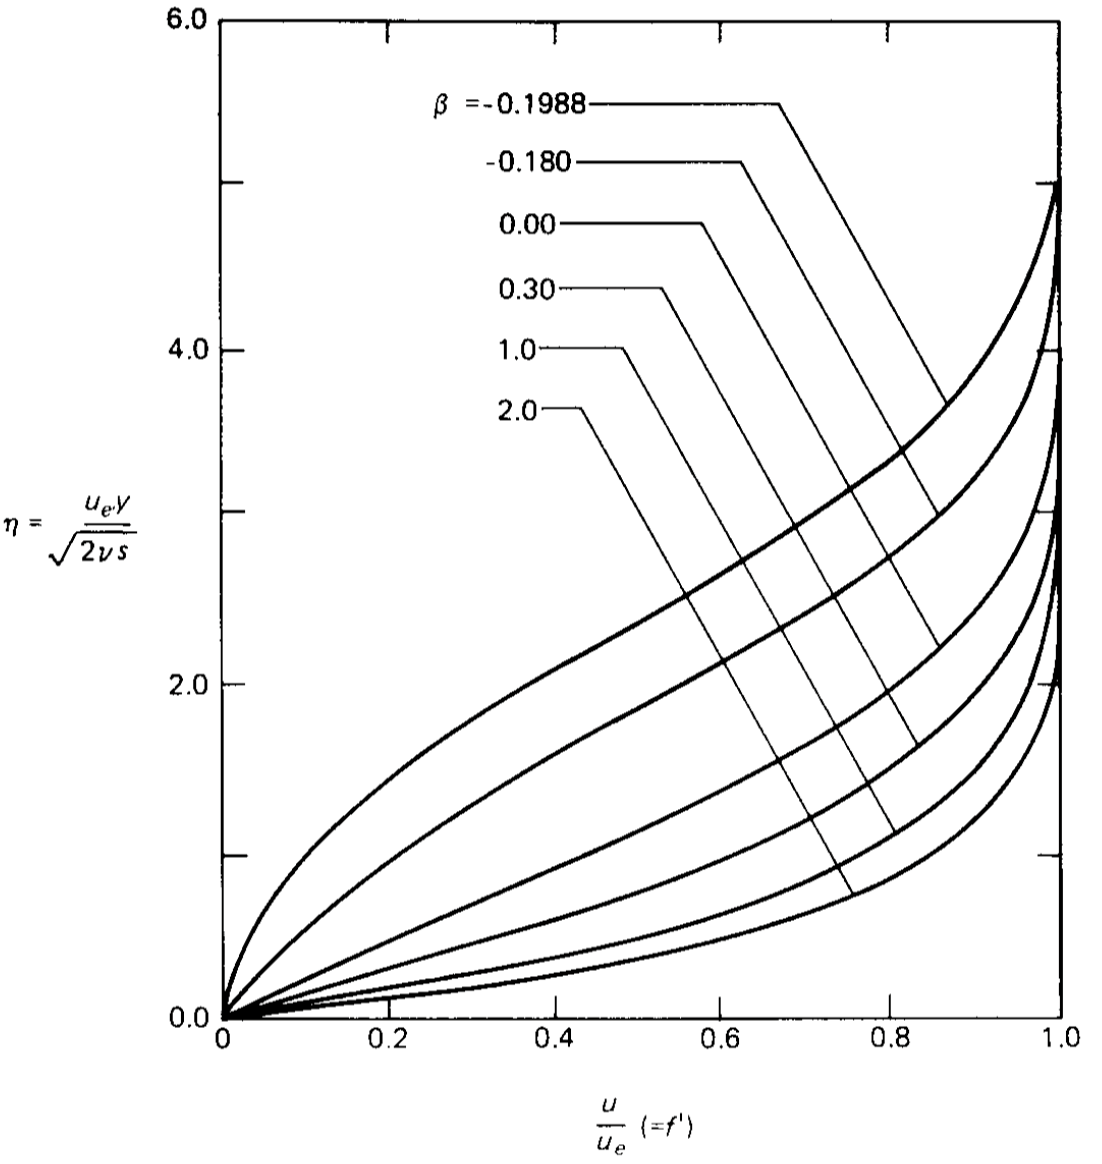
\includegraphics[scale=0.20]{ch5/13}
	\captionof{figure}{}
\end{center}
	\label{fig:5.13}
	\end{minipage}
	\begin{minipage}{0.49\textwidth}
\begin{center}
	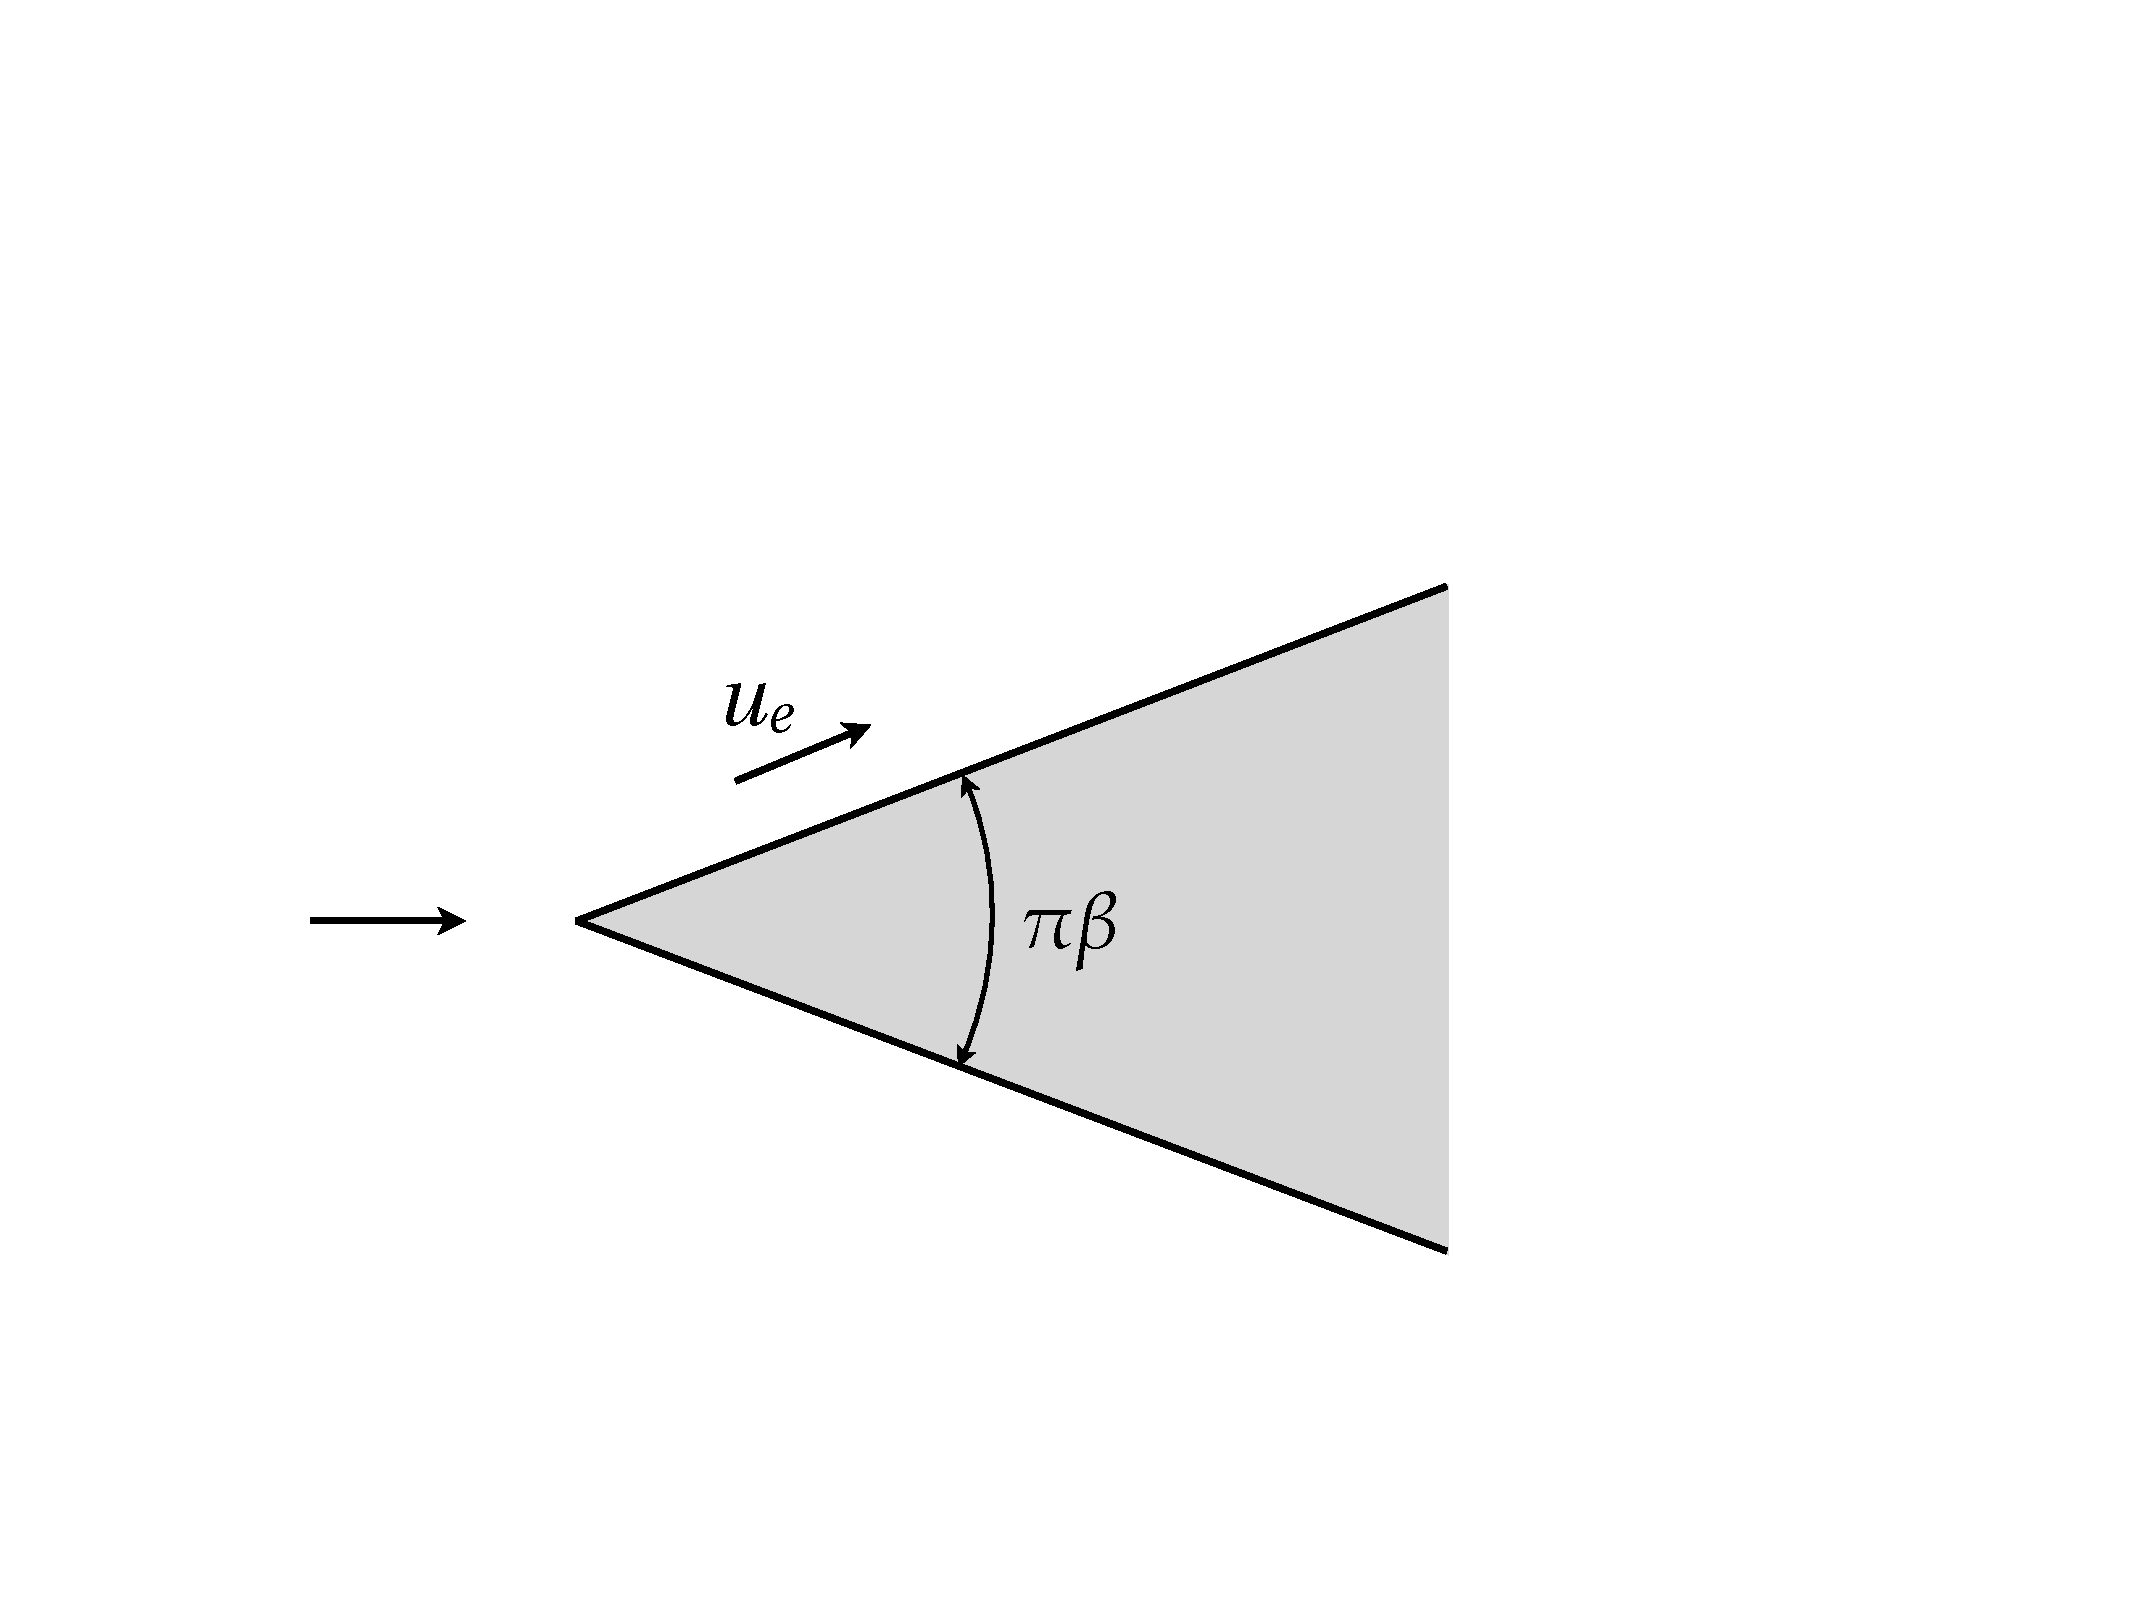
\includegraphics[scale=0.34]{ch5/14}	
	\captionof{figure}{}
\end{center}
	\label{fig:5.14}
	\end{minipage}
	\end{center}
	
			\autoref{fig:5.13} represents these profiles in function of $\beta$. $\beta = 0$ is the zero pressure gradient. For increasing $\beta$ the boundary layer gets stiller and the profile fuller. When $\beta$ decelerate, the boundary layer gets thickker and the velocity profile has an inflexion point. For $\beta > -0.1988$, the curve starts with a vertical tengent $\frac{du}{dy} = 0$, no friction. We could imagine this is good but in fact for these values there is separation of the boundary layer (reversed flow). Now we will answer to two questions:\\
			
			\begin{itemize}
				\item[•] do this $x$ law velocity profile have a physical meaning?\\
				It turns out that $u_e = a x^m$ is the velocity disctribution over a wedge where the opening angle is precisly equal to 

				\begin{equation}
					\frac{2m}{1+m} \pi = \pi \beta .
				\end{equation} 
				
					When $\beta > 0$ this is an easy practical case represented on \autoref{fig:5.14}. In particular, $\beta =1$ corresponds to $m=1$ and an opening angle $\pi$. This is the flow near a stagnation point. Indeed, $m = 1$ means that 
					
					\begin{equation}
						\frac{du_e}{dx} = a = cst \qquad \Rightarrow l^2 = \frac{\nu}{a} \neq 0 
					\end{equation}
					
					meaning that the boundary layer does not start at 0 thickness at a stagnation point. \\
				
				\item[•] what can we do when this profile is not the case. \\
				Let's make a qualitative discussion on the influence of pressure on the velocity profile. 
			\end{itemize}			   
			
			
\section{Effect of pressure gradient on velocity procile in a boundary layer - qualitative analysis}
		
	\begin{wrapfigure}[6]{l}{6.5cm}
	\vspace{-5mm}
	\begin{tabular}{c|ccccc}
	 $y$ & $u$ & $\frac{\D u}{\D y}$ & $\frac{\D ^2 u}{\D y^2}$ & $\frac{\D ^3 u}{\D y^3}$ & $\frac{\D ^4 u}{\D y^4}$ \\
	 \hline 
	 	 \ \\ $0$       & 0 & $\frac{\tau _w}{\mu}$ & $\frac{1}{\mu}\frac{\D p}{\D x}$ & 0 & $\frac{1}{\nu \mu ^2}\tau _w \frac{\D\tau _w}{\D x}$  \\ \\
	 $\delta$ & $u_e$ & 0 & 0 & 0 & 0 \\ 
	 \hline 
	 \end{tabular}  
	 \captionof{table}{}
	 \label{table:5.1}
	 \end{wrapfigure}
	We want to sketch the velocity profile as a function of pressure gradient. \autoref{table:5.1} lists the value of the velocity and its derivative at the wall and the boundary layer edge. At $\delta$, because of the bigger thickness scale in the outer region, the slope of $u = 0$. For $\frac{du}{dy}$, we use the shear stress at the wall

	\begin{equation}
		\tau _w = \left. \mu \frac{\D u}{\D y}\right| _w
	\end{equation}
	
	For $\frac{\D ^2 u}{\D y^2}$, we use the momentum equation computed at the wall
	
	\begin{equation}
		\nu \left.\frac{\D ^2 u}{\D y^2}\right| _w = \frac{1}{\rho}\frac{\D p}{\D x} \qquad \Rightarrow \left.\frac{\D ^2 u}{\D y^2}\right| _w  = \frac{1}{\mu}\frac{\D p}{\D x}
	\end{equation}
	
	For the third order, we will differentiate the momentum equation \eqref{eq:5.44} with respect to y. This gives
	
	\begin{equation}
	\begin{aligned}
		&u \frac{\D ^2 u}{\D x \D y} + \frac{\D u}{\D y}\frac{\D u}{\D x} + \frac{\D v}{\D y} \frac{\D u}{\D y} + v \frac{\D ^2 u}{\D y^2} =0+ \nu \frac{\D ^3 u}{\D y^3}\\
		\Leftrightarrow  \qquad
		&u \frac{\D ^2 u}{\D x \D y} + \frac{\D u}{\D y}\underbrace{\left(\frac{\D u}{\D x} + \frac{\D v}{\D y}\right)}_{=0 \mbox{ continuity }} + v \frac{\D ^2 u}{\D y^2} =0+ \nu \frac{\D ^3 u}{\D y^3} \\
		\Leftrightarrow  \qquad 
		&u \frac{\D ^2 u}{\D x \D y} + v \frac{\D ^2 u}{\D y^2} =  \nu \frac{\D ^3 u}{\D y^3} \qquad \Leftrightarrow \nu \left.\frac{\D ^3 u}{\D y^3}\right| _w = 0 
	\end{aligned}
	\end{equation}
	
	To have the fourth derivation we need to derive one more time 
	
	\begin{equation}
	\begin{aligned}
	&u \frac{\D ^2 u}{\D x \D y} + \frac{\D u}{\D y}\underbrace{\left(\frac{\D u}{\D x} + \frac{\D v}{\D y}\right)}_{=0 \mbox{ continuity }} + v \frac{\D ^2 u}{\D y^2} =0+ \nu \frac{\D ^3 u}{\D y^3} \\
		\frac{\D}{\D y}\Rightarrow  \qquad 
		&\frac{\D u}{\D y}\frac{\D ^2 u}{\D x \D y} +  u\frac{\D ^3 u}{\D x \D y^2} + v \frac{\D ^3 u}{\D y^3} + \frac{\D v}{\D y} \frac{\D ^2 u}{\D y^2} = \nu \frac{\D ^4 u}{\D y^4} \\
		\Leftrightarrow \qquad &\frac{\tau _w}{\mu}\frac{\D}{\D x}\left(\frac{\tau _w}{\mu}\right) + 0 + 0 +  0 = \nu \left.\frac{\D ^4 u}{\D y^4}\right| _w \qquad \Rightarrow \left.\frac{\D ^4 u}{\D y^4}\right| _w = \frac{1}{\nu \mu ^2}\tau _w \frac{\D\tau _w}{\D x}
	\end{aligned}
	\end{equation}
	
	\begin{wrapfigure}[8]{l}{6.7cm}
	\vspace{-5mm}
	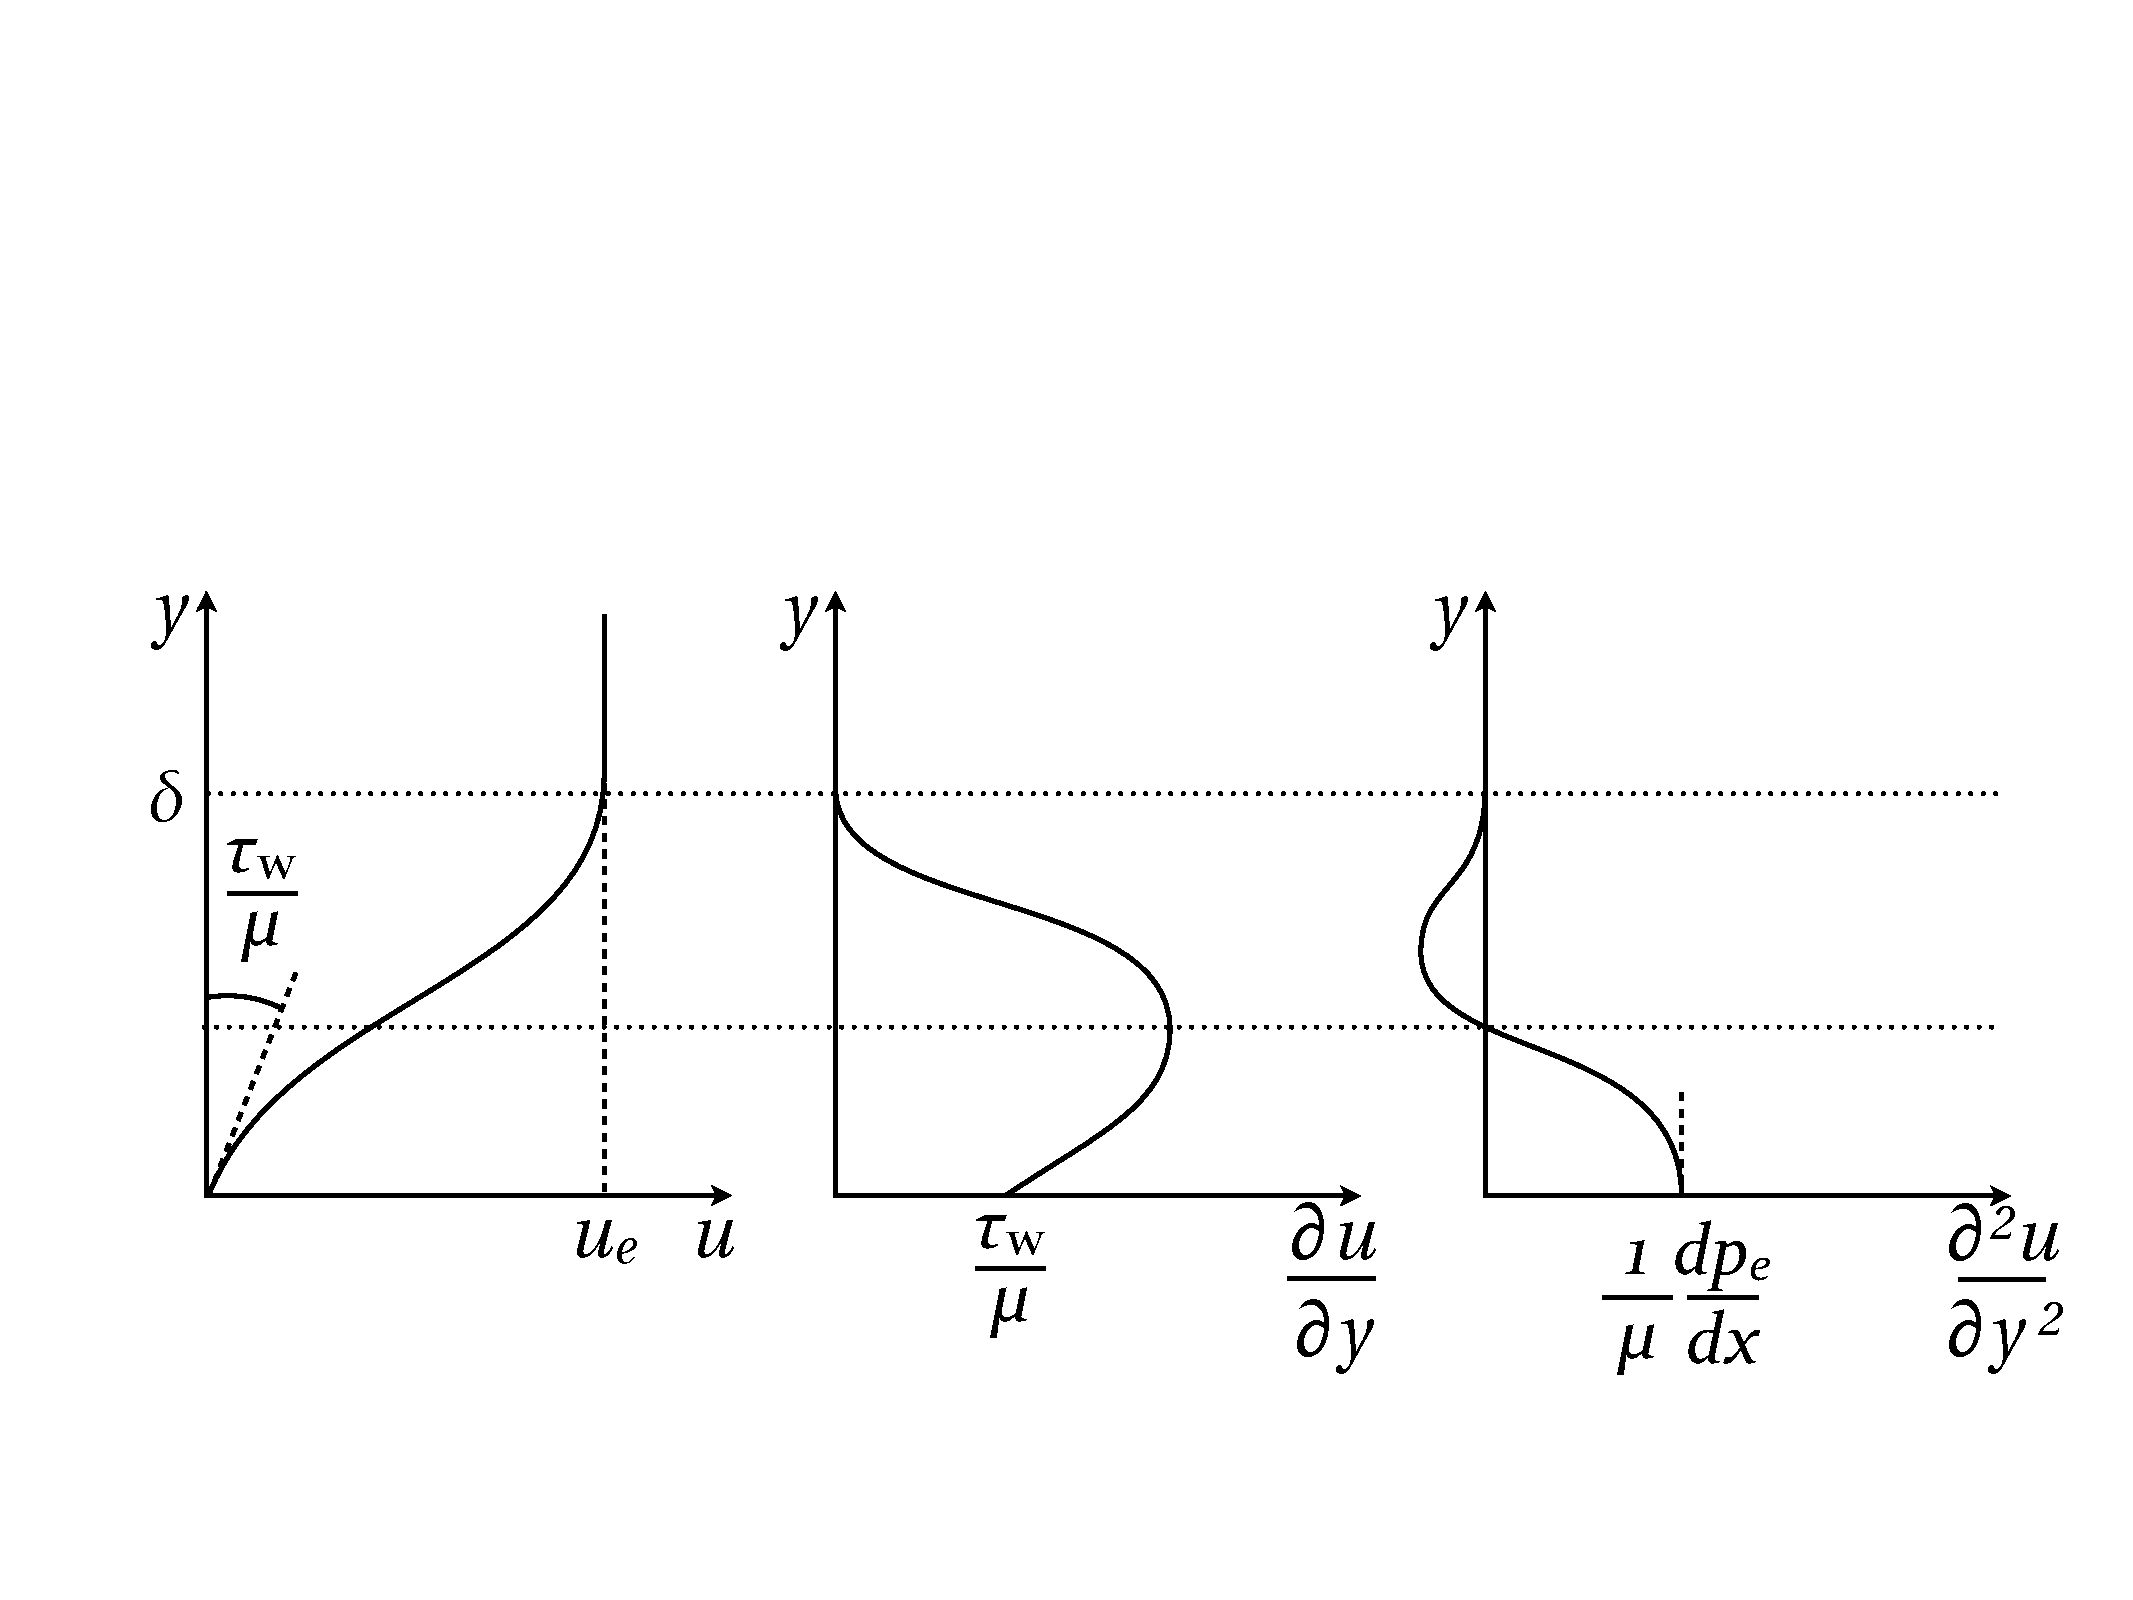
\includegraphics[scale=0.2]{ch5/15}
	\captionof{figure}{}	
	\label{fig:5.15}
	\end{wrapfigure}
	Now we will plot the derivative in function of $y$ in the case of decelarating flow so a positive pressure gradient. Let's suppose that $\tau _w >0$, as the second derivative is positive, it means that the first derivative increases with $y$. The third derivative beeing equal to 0, the second derivative begins with a slope 0. The first derivative has to reach the value 0, it means that we need a maximum where the derivative is equal to 0 (second derivative vanishes there), meaning that \textbf{in the velocity profile we have a inflexion point where we reach a maximum before continuing to increase}. We founded that before but now we conclude that it's a general case for $\beta <0$. We also see that the second derivative curvature becomes negative, meaning that 
	
	\begin{equation}
		\frac{\D ^4 u}{\D y^4} <0 \qquad \Rightarrow \frac{\D \tau _w}{\D x} < 0
	\end{equation}
			
	So we have \textbf{a tendancy for decreasing shear stress}. This is confirming what we found in the power law. The presence of the inflexion point makes the boundary layer unstable for disturbancies, it makes it switched to turbulencies more easely (promote transition to turbulence, increased friction). The decresing shear stress can be seen as good but in fact, when shear stress vanishes, separation appears (promote separation). So the conclusion is that we have a lot of bad phenomena for increasing pressure, this is why we call that the \textbf{adverse pressure gradient} when positif. 
	
%%%%%%%%%%%%%%%%%%%%%%%%%%%%
%	Ch5 : Boundary layer (Suite par Michael Benizri) %
%%%%%%%%%%%%%%%%%%%%%%%%%%%%

\section{Approximate solution method for boundary layers (integral method)}
\subsection{Balances}

\begin{wrapfigure}[8]{l}{6cm}
\vspace{-5mm}
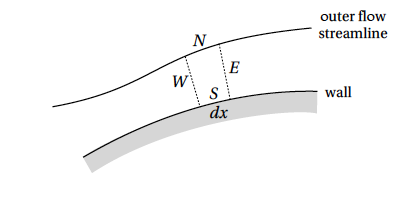
\includegraphics[scale=0.2]{ch5/16}
\captionof{figure}{}
\end{wrapfigure}


\footnote{Continued by Michael Benizri.} When we have an outer velocity wich is not a power low, we don't have a self-similar solution of the boundary equation. The idea of integral methods is to give up the objective of determining the detailed velocity field (this is what we need in the equations) but rather to restrict our objective to finding the following global quantities: the skin friction $C_f(x)$, the momentum thickness $\theta (x)$ and the displacement thickness $\delta ^*(x)$.

How? By making semi-global balances. We are going to make balances on an infinitesimal slice of lenght $dx$ on an outer flow streamline. So it remains local in the tangential direction ($dx$ is infinitesimal) but it is global in the normal direction (the balance is over the whole boundary layer).

\subsubsection{Mass balance} 
It's a steady flow problem so the mass balance consist in saying that the total mass flow out is equal to the zero. Let's then compute the mass flow on each side of the de $dx$ element. First, there is no mass flow over S because of the solid body and no flow over N follows the streamline and this last is defined as beeing tengential to the velocity 

\begin{equation}
	N : \dot{m}_N=0 \qquad S : \dot{m}_S=0
\end{equation}
For the West and East side, we have to apply the definition of mass flow, where\footnote{W is on $x$ and E on $x+dx$} $ds = dy$ is a curve element, $\vec{n}_E=\vec{e}_x$ and $\vec{n}_W=-\vec{e}_x$

\begin{equation}
\begin{aligned}
&E: 	\qquad\dot{m}_E= \int_{E} \rho (\vec{u}.\vec{n})\,  d s  
		= \int_{0}^{y(x+dx)} \rho u \, d y \\ 
&W: \qquad\dot{m}_W= \int_{W} \rho (\vec{u}.\vec{n})\, d s  
		 = -\int_{0}^{y(x)} \rho u \,d y  
		\end{aligned}
\end{equation}

By applying the balance we get
\begin{equation}
\int_{0}^{y(x+dx)} \rho u \, d y - \int_{0}^{y(x)} \rho u \, d y =0\qquad \Leftrightarrow \qquad dx \frac{d}{dx} \int_{0}^{y(x)} \rho u \, d y =0 
\end{equation}

Where the left term has been transformed using the definition of a derivative.
By simplifying $dx$, considering a constant density flow, the fact that $u_{e}$ is only a function of x, the definition of the displacement thickness $\delta^*$ and by using a small trick, we get

\begin{equation}
\frac{d}{dx} \int_{0}^{y(x)} \rho u \, dy = \rho \int_{0}^{y(x)}  (u-u_e+u_e) \, dy = \rho u_e y  -\rho \underbrace{\int_{0}^{y(x)}  (u_e-u) \, dy}_{u_e\delta ^*} = \rho u_e(y-\delta^*)
\end{equation}

Finally, we end up with the

\begin{center}
\theor{
\textbf{Mass flow balance}
\begin{equation}
\frac{d}{dx} \int_{0}^{y(x)} \rho u \, dy = \frac{d}{dx}\rho u_e(y-\delta^*) = 0
\end{equation}
}
\end{center}

\subsubsection{Tangential momentum balance (x-wise)}

\textit{Total tangential momentum flow out = sum of tangential forces.}
\\

The momentum flow is the mass flow times the velocity. Therefore, if there is no mass flow, there is no momentum flow for N and S. For E and W, the previous expressions simply becomes

\begin{equation}
\begin{aligned}
&E: \qquad
		\dot{p}_{xE}= \int_{E} \rho u (\vec{u}.\vec{n}) d s  
		= \int_{0}^{y(x+dx)} \rho u^2 \, dy  \\
&W: \qquad
		\dot{p}_{xW}= \int_{W} \rho u (\vec{u}.\vec{n})\, d s  
		= - \int_{0}^{y(x)} \rho u^2 \, dy  
		\end{aligned}
\end{equation}

By putting those two terms together and by using the definition of the derivative

\begin{equation}
\dot{p}_{xE}+\dot{p}_{xW} = \int_{0}^{y(x+dx)} \rho u^2 \, dy - \int_{0}^{y(x)} \rho u^2 \, dy  =dx \frac{d}{dx} \int_{0}^{y(x)} \rho u^2 \, dy
\end{equation}

Let's now compute the forces:\\

\begin{itemize}
\item[•] S: We have the shear stress (friction) $\tau_w$ which applies over a length $dx$ and slows down the fluid
\begin{equation}
	F_s = -\tau_w dx
\end{equation}  

\item[•] W: We have a pressure force defined and applicated to W as
\begin{equation}
F_p=- \int p \vec{n} \, d s \Rightarrow  F_{xW}=- \int_W p n_x\, d s=-\int_0^{y(x)} p (-1) \, dy=[p_e y]_{y(x)}
\end{equation}

where the last expression is allowed because we previously found that pressure gradient in BL is negligible. \\

\item[•] E: We also have a pressure force and it is exactly the same principle
\begin{equation}
F_p=- \int p \vec{n} \,d s \Rightarrow  F_{xE}=- \int_E p n_x \,d s=-\int_0^{y(x+dx)} p (1) \, dy=-[p_e y]_{y(x+dx)}
\end{equation}
	
Using the definition of the derivative for W and E contributions, we get

\begin{equation}
F_w+F_E=- dx \frac{d}{dx} (p_e y)
\end{equation}

\item[•] N: This corresponds to the inviscid flow region so there is no shear stress. However, there is a pressure force due to the streamline non parallel to the wall.\\
\end{itemize}

\begin{wrapfigure}[11]{l}{2.5cm}
\vspace{-7mm}
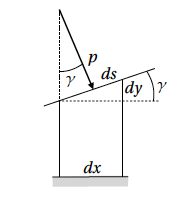
\includegraphics[scale=0.25]{ch5/17} 
\captionof{figure}{}
\end{wrapfigure}

So we apply the common pressure definition, knowing that $dx$ is infinitesimal so there is no need of an integral 

\begin{equation}
F_{xN}=- \int_N p n_x \,d s =-p n_x \, d s =-p(-\sin \gamma)\, ds=p \, dy=p \frac{dy}{d x} dx
\end{equation}
\ \\

Let's now put everything together:

\begin{equation}
\cancel{dx} \frac{d}{dx} \int_{0}^{y(x)} \rho u^2 \, dy=-\tau_w \,\cancel{dx}-\cancel{dx} \frac{d}{dx}(p_ey)+p \frac{d y}{d x} \cancel{dx} \Leftrightarrow  \frac{d}{dx} \int_{0}^{y(x)} \rho u^2 \, dy=-\tau_w - y\frac{dp_e}{dx}
\end{equation}

By applying the same trick as used for the mass conservation, we get

\begin{equation}
\begin{aligned}
\int_{0}^{y(x)} \rho u^2 \, dy &= \rho \int_{0}^{y(x)}  (u^2-uu_e+uu_e-u_e^2+u_e^2) \, dy\\
&=\rho \left[u_e^2y-u_e^2 \int (1-\frac{u}{u_e})dy-u_e^2 \int (\frac{u}{u_e})(1-\frac{u}{u_e})dy\right] = \rho u_e^2[y-\delta^*-\theta]
\end{aligned}
\end{equation}

Remember that mass conservation tells us that $\rho u_e(y-\delta^*)$ is a constant. Then we have, by entering our last result in the momentum equation

\begin{equation}
\rho u_e(y-\delta^*)\frac{d u_e}{d x}- \frac{d}{d x} \rho u_e^2\theta =,-\tau_w-y \frac{d p_e}{d x} 
\end{equation}

From the inviscid momentum equation we had $
- \frac{1}{\rho}\frac{d p_e}{d x} = u_e \frac{d u_e}{d x}$. Therefore, by eliminating the terms in $y$, we have

\begin{equation}
 \rho u_e\delta^* \frac{d u_e}{d x}+ \frac{d}{d x} \rho u_e^2 \theta=\tau_w
\end{equation}

We obtain an equation that is independant of y. That means that we have found an equation that is independant of the choice of the streamline.

By using the fact that: $ \frac{d}{d x} \rho u_e^2 \theta = \rho u_e^2 \theta (\frac{d}{d x} \log(u_e^2 \theta))=\rho u_e^2 \theta(2\frac{d u_e}{u_e d x}+\frac{d \theta}{\theta d x})$ and dividing all the terms by $\rho u_e^2 $ to get a non dimensionnal form. We get the

\begin{center}
\theor{
\textbf{Karman's integral equation}
\begin{equation}
\frac{d \theta}{d x}+(\delta^*+2 \theta)\frac{d u_e}{u_e d x}=\frac{\tau_w}{\rho u_e^2}=\frac{C_f}{2}
\label{eq:5.81}
\end{equation}
}
\end{center}

This is an exact equation, we made no approximation, but $\delta ^* and \theta$ still depends on the velocity profile (velocity profile is hidden). The idea is now to make some assumption on the shape of the velocity profile to solve this equation.

\subsection{Solving Karman's integral equation}

\begin{wrapfigure}[9]{l}{3.5cm}
\vspace{-5mm}
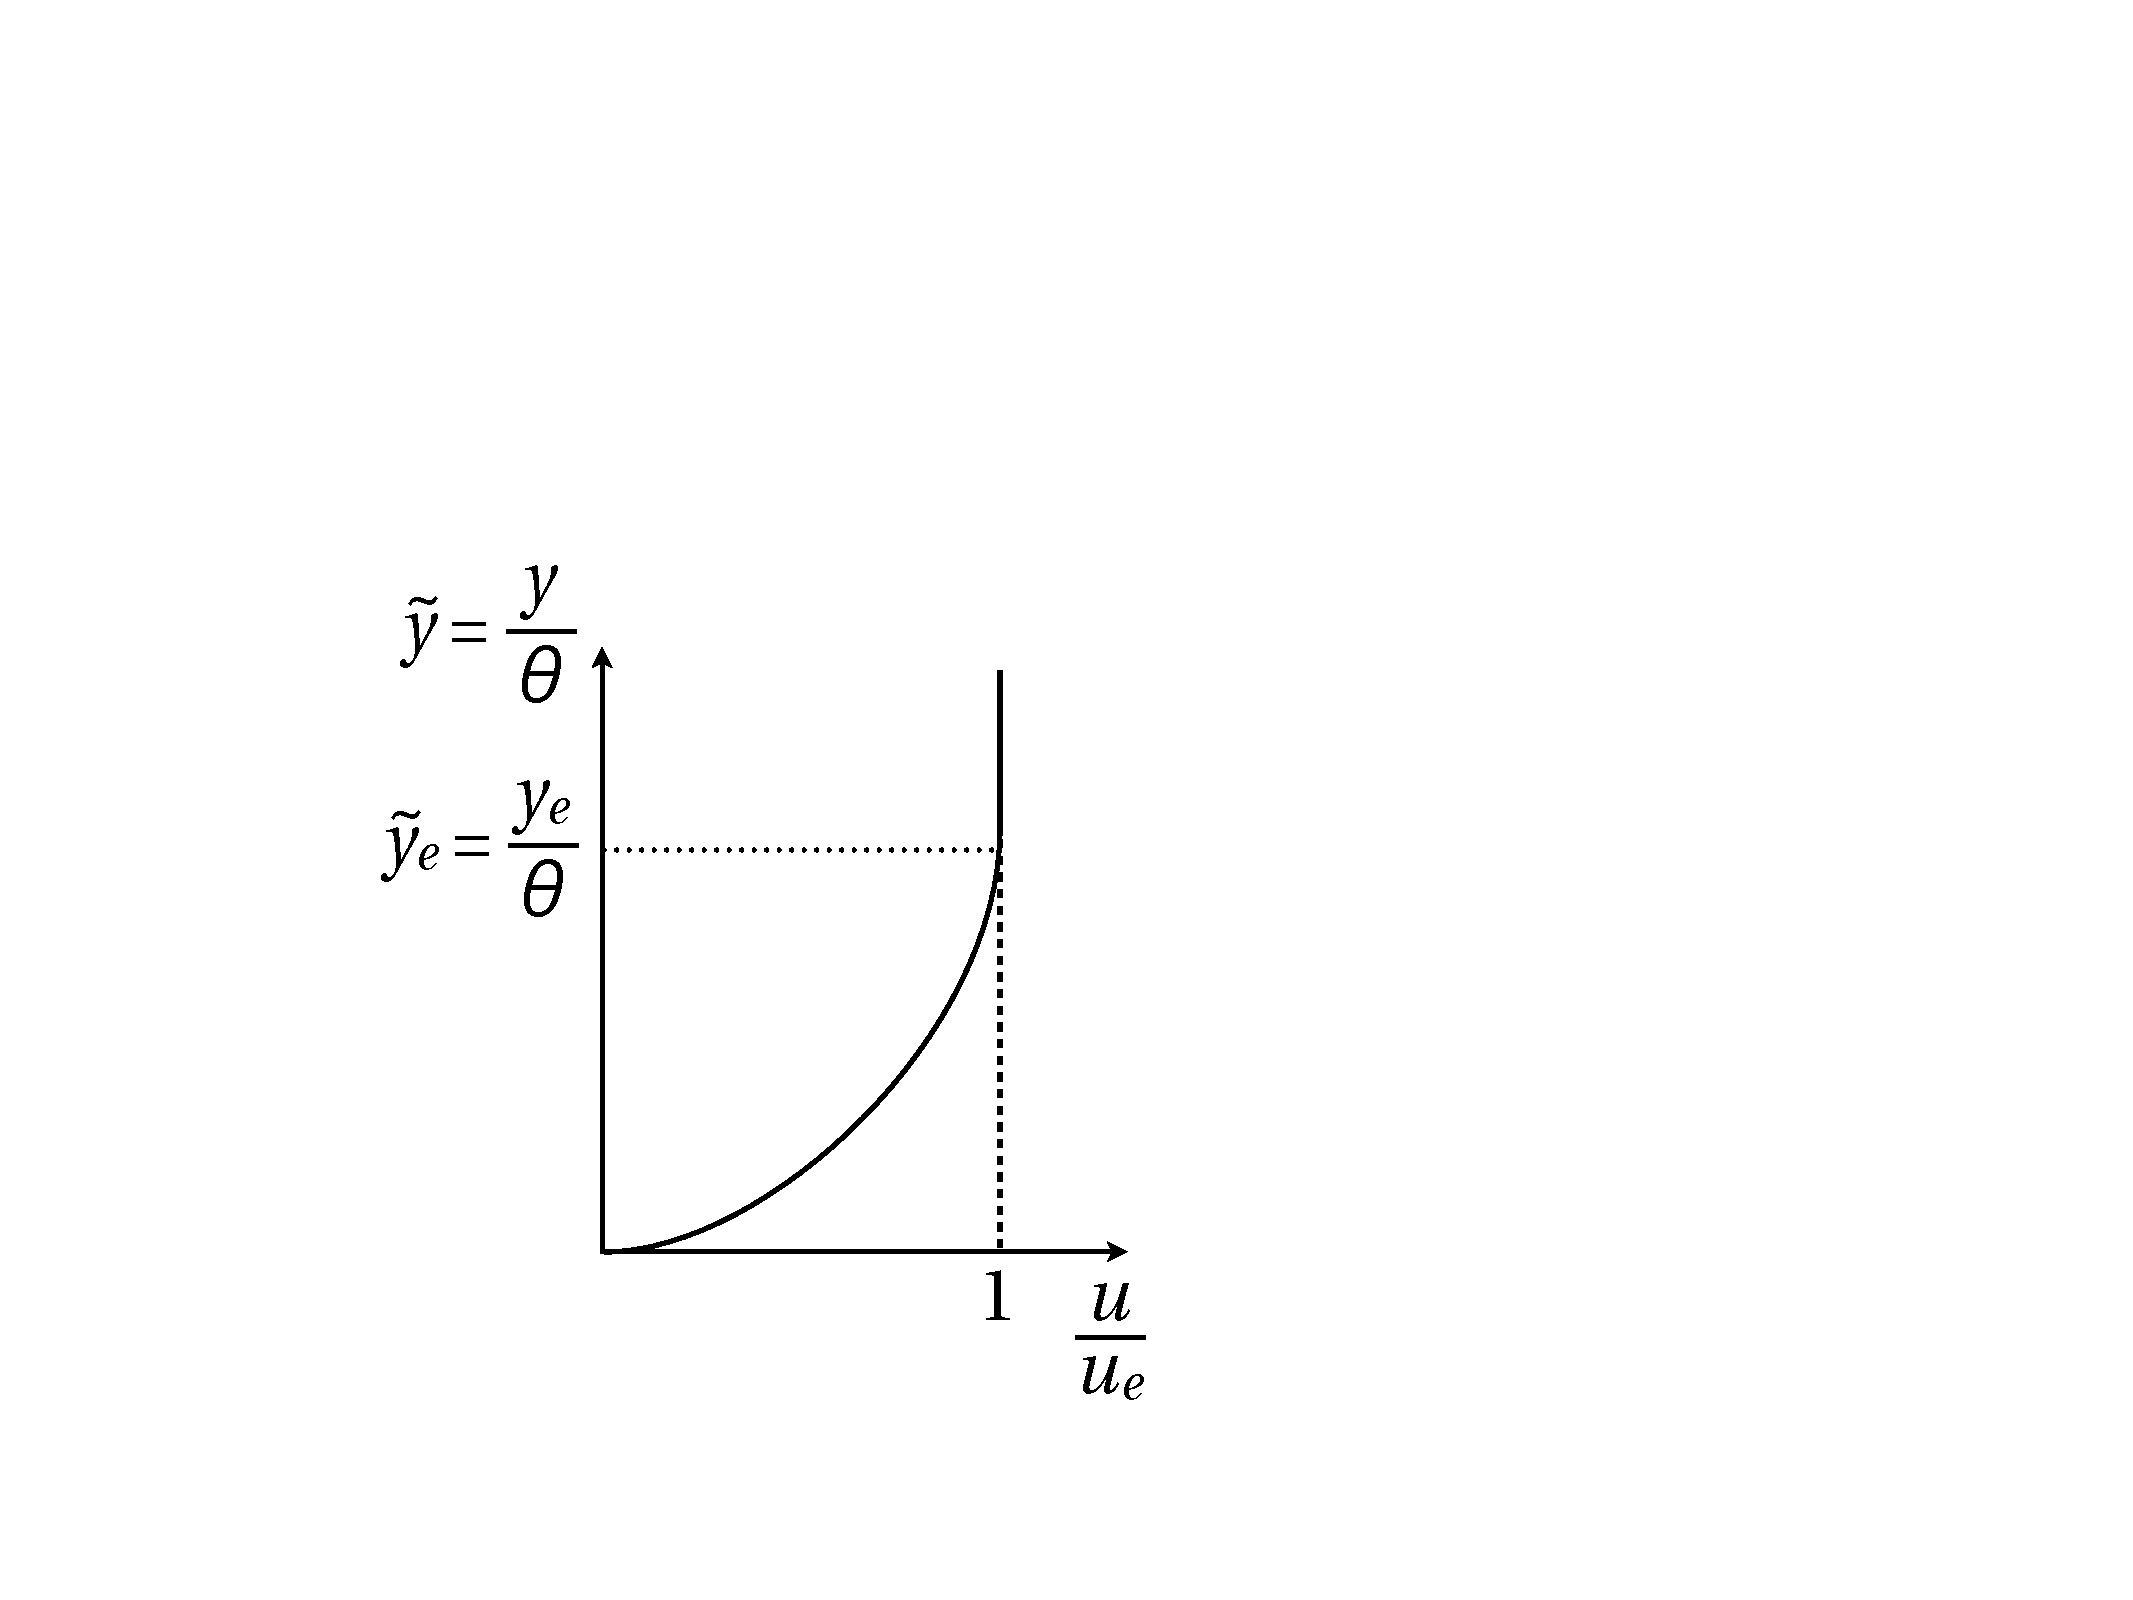
\includegraphics[scale=0.25]{ch5/19}
\captionof{figure}{}
\label{fig:5.18}
\end{wrapfigure}
We have to make assumptions on the velocity profile to solve this equation. Let's firts make a dimensionnal analysis
\begin{equation}
u=F(u_e,y,\nu,\theta) \rightarrow \frac{u}{u_e}=f(\frac{y}{\theta}=\tilde{y},\cancel{\frac{u_e \theta}{\nu}=R_{e \theta}})
\end{equation}

Remember that for a laminar flow, the Reynolds number does not play a role. With that we assume that there is a unique velocity profile as in \autoref{fig:5.18}. So we will first make this assumption $\frac{u}{u_e} = f\left(\frac{y}{\theta}\right)$. If we take the definition of $\delta ^*$ which is

\begin{equation}
\delta^*=\int_0^\infty (1-\frac{u}{u_e}) \, dy,
\end{equation}

by multiplying by $\frac{\theta}{\theta}$ and by using $\frac{u}{u_e}=f(\tilde{y})$, we get

\begin{equation}
\delta^*=\theta \int_0^\infty (1-\frac{u}{u_e}) \frac{d y}{\theta}=\theta \underbrace{\int_0^\infty (1-f(\tilde{y})) \, d \tilde{y}}_{H} = \theta H
\end{equation}

Where H is the \textbf{velocity shape factor} and is constant . This final equation, as $\delta ^*$ and $\theta$ are related, eliminates one unknown.

Let's now look to the stream friction coefficient

\begin{equation}
\frac{C_f}{2}=\frac{\tau_w}{\rho u_e^2}=\frac{\mu \frac{\partial u}{\partial y}|_0}{\rho u_e^2}=\frac{\nu u_e f'(0)}{u_e^2 \theta}=\frac{1}{R_{e \theta}} f'(0)=\frac{T}{R_{e \theta}}
\end{equation}

In this equation we used the dimensional analysis which gives us:
$\frac{u}{u_e}=f(\tilde{y}) \rightarrow \frac{\partial u}{\partial y}=u_e f'(\tilde{y}) \frac{1}{\theta}$.

Where we define another constant $T=f'(0)$. This closes the problem, making $C_f$ dependent on $\theta$ and reducing unknowns number from 3 to 1. But the assumption is not physically realistic because it boils down to assuming self similarity which is not necessary the case. The hypothesis has to be complexified to consider a family of velocity profiles that can be labelled by a number (the identification parameter K) and K will be the \textbf{identification parameter} in order to have a one to one matching with the velocity profiles. The only changing thing is that now 

\begin{equation}
\frac{u}{u_e} = f(\frac{y}{\theta}, K) \qquad \Rightarrow \qquad \delta^*=\theta H(K) \quad and \quad \frac{C_f}{2} = \frac{T(K)}{Re_\theta}
\label{eq:5.86}
\end{equation}

where H and T become funtion of K. So now we have one equation and two unknowns, one equation is then missing.
\\

To find a complementary equation, we can:
\begin{enumerate}
\item Make another global balance, e.g. kinetic energy balance. This will give a set of ordinary differantial equation easily solved by Matlab. This method is the only accurate one for \textbf{turbulent flows}. In this case we will choose $H$ to label the profiles. 

\item For a laminar flow, we can compute the local momentum equation at one point in the BL (the wall $y=0 \Rightarrow u=v=0$)). There, the momentum equation using no-slip condition becomes 
\begin{equation}
	\left.\frac{\nu  \partial^2 u}{\partial y}\right|_0=-u_e\frac{du_e}{dx}
\end{equation}
and by using the funtion $\frac{u}{u_e} = f(y/\theta , K)$, we get

\begin{equation}
 \frac{\nu}{\theta^2}u_e f''(0,K) =-u_e \frac{d u_e}{d x}\qquad  \Leftrightarrow \qquad  -f''(0,K)=\frac{\theta^2}{\nu} \frac{d u_e}{d x}
\end{equation}

The final result gives an algebraic relation linking K and $\theta$ and not a differantial one like the other method. We can choose to be the label $K=-f''(0,K) $. Then we have 
\begin{equation}
K=\frac{\theta^2}{\nu} \frac{d u_e}{d x}
\end{equation} 
where we can see that $K>0$ corresponds to an accelerating flow vice-versa
\end{enumerate}

Let's now take Karman's integral equation \eqref{eq:5.81} and mutliply by $Re_{ \theta}=\frac{u_e \theta}{\nu}$, using \eqref{eq:5.86} and after some manipulations, we get

\begin{center}
\theor{
\textbf{Thwaites}
\begin{equation}
\begin{aligned}
&\frac{u_e d \left(\frac{\theta^2}{\nu}\right)}{2 d x}=T(K)-K (2+H(K)) \equiv\frac{F(K)}{2}\\
&\frac{u_e d \left(\frac{\theta^2}{\nu}\right)}{d x}=F(K)=a-bK
\end{aligned}
\end{equation}
}
\end{center}

We now have to specify the velocity profile to continue.

\subsubsection{Choice of the velocity profile}
Historically, the first idea was to use a polynomial fit of order 4, but Thwaites demonstrated experimentally that there is no need to know the velocity profile as the experimental points fitted a first order line. This is perfect for turbulent flows where we don't exactly know the profile. Let's take back the Thwaites equation in which we define $Z=\frac{\theta^2}{\nu}$, we get by dividing by $u_eZ$

\begin{equation} 
\begin{aligned}
&u_e\frac{d Z}{d x}+ bZ\frac{d u_e}{d x}=a \qquad \Rightarrow \frac{d Z}{Z d x}+b \frac{d u_e}{u_e d x}=\frac{a}{u_eZ}  = \frac{d }{d x} ln(Zu_e^b) = \frac{1}{Zu_e^b}\frac{d }{d x} \\
&\Rightarrow \qquad \frac{1}{Zu_e^b}\frac{d }{d x} (Zu_e^b)=\frac{a}{u_eZ} \qquad  \Leftrightarrow \qquad \frac{d }{d x} (Zu_e^b)=au_e^{b-1}\\
&\Rightarrow \qquad Z(x)=\frac{\theta^2(x)}{\nu}=\frac{a}{u_e^b(x)}\left[\int_0^x u_e^{b-1}(s) d s +c\right]
\end{aligned}
\end{equation}

Where we take c=0. As a matter of fact, if the stagnation point is taken as the origin of the coordinate system, since $x=0$ at a stagnation point, we get $c=0$. So finally we have

\begin{equation}
 Z(x)=\frac{\theta^2(x)}{\nu}=\frac{a}{u_e^b(x)}\int_0^x u_e^{b-1}(s) d s \qquad and \qquad K(x) = Z(x) \frac{du}{dx}
\end{equation}

This equation has a singular point at the stagnation point, where the behaviour is

\begin{equation}
\lim_{x \rightarrow 0} \frac{\theta^2}{\nu}=a \lim_{x \rightarrow 0} \frac{u_e^{b-1}(0)}{bu_e^{b-1}(0) u'_e(0)} \qquad\Leftrightarrow \qquad \left.\frac{\theta^2}{\nu}\right|_{stag.point}=\frac{a}{bu'_e(0)}
\end{equation}

This solution is similar to the one obtained with the self-similar solution.
This method is simple but is only valid for laminar flows. Accuracies varies between  5\%  and 15\% which is not bad considering the simplicity of the method.

\section{Viscous-Inviscid interactions}

According to the Thwaites relation, K (and so the velocity profile) depends only on the outer velocity distribution, and is independent of the viscosity and of the Reynolds number. The separation point location is then independent of the viscosity and therefore on the Reynolds number. This is in contradiction with experiments. A possible explanation is that the displacement effect induces a pressure disturbance, that has to be taken into account by imposing normal velocity matching.\\

Furthermore, the computed separation is oftentimes way of the experimental location. What could be the source of the problem?
\begin{enumerate}
\item Approximate character of integral methods ? NO
\item Boundary layer theory incorrect ? NO
\item Normal velocity mismatch (displacement effect) ? Let's check!
\end{enumerate}

The normal velocity mismatch is expected to modify the pressure distribution over the body $u_e(x)=u_e(x)+\delta u_e(x)$, where $\delta u_e(x)$ is the perturbation due to the displacement effect depending on Re.\\

That this is indeed the reason for the discrepancy between theory and experiment is confirmed by the good agreement between theory and experiment if the BL calculations is performed using the experimental pressure distribution. CURE: Impose normal velocity matching!
\\

Normal velocity matching: $ v_e(x,y)=v^{inv}(x,y)$ at some $y \ge \delta$. 

\subsubsection{Reminder of integral methods}
\begin{equation}
\frac{d}{d x} \int_0^{y(x)} \rho u \, dy =\rho \frac{d}{d x} u_e (y-\delta^*)=0
\end{equation}

By developping the right hand side we get
\begin{equation}
\rho \frac{d}{d x} u_e (y-\delta^*)=u_e \frac{d y}{d x} +y  \frac{d u_e}{d x} - \frac{d}{d x} (u_e\delta^*)
\end{equation}

For a streamline: $  \frac{v_e}{u_e}=\frac{d y}{d x}$

By imposing velocity matching, we get:

\begin{equation}
u_e\frac{d y}{d x}=v_e(x,y)=\frac{d}{d x} (u_e\delta^*)-y\frac{d u_e}{d x}=v^{inv}(x,y)
\end{equation}

Let's extrapolate the outer inviscid flow inside the BL:

\begin{equation}
\frac{\partial u^{inv}}{\partial x}+\frac{\partial v^{inv}}{\partial y}=0 \Leftrightarrow \frac{\partial v^{inv}}{\partial y}=-\frac{\partial u^{inv}}{\partial x} 
\end{equation}

\begin{equation}
\int_z^y \frac{\partial v^{inv}}{\partial \zeta} d\zeta=v^{inv}(x,y)-v^{inv}(x,z)=\int_z^y \frac{\partial u^{inv}}{\partial x} d\zeta \quad where \quad \frac{\partial u^{inv}}{\partial x}=\frac{d u_e}{d x}
\end{equation}

Therefore, we get:
\begin{equation}
v^{inv}(x,y)-v^{inv}(x,z)=-\frac{d u_e}{d x} (y-z) \quad where \quad v^{inv}(x,y)=\frac{d}{d x} (u_e\delta^*)-y\frac{d u_e}{d x}
\end{equation}

Finally, we get:
\begin{equation}
v^{inv}(x,z)=\frac{d}{d x} (u_e\delta^*)-z\frac{d u_e}{d x}
\end{equation}

There are two interesting points:
\begin{enumerate}
\item $z=0:
v^{inv}(x,0)=\frac{d}{d x} (u_e\delta^*) \quad$ Transpiration velocity model
\item $z=\delta^*: 
v^{inv}(x,\delta^*)=\frac{d}{d x} (u_e\delta^*)-\delta^*\frac{d u_e}{d x}= u_e \frac{d \delta^*}{d x} \quad$ Displacement surface model
\end{enumerate}

We can rewrite case of $z=\delta^*$ in another form:
\begin{equation}
\frac{v^{inv}(x,\delta^*)}{u_e}=\frac{d \delta^*}{d x}
\end{equation}

This shows that the outer inviscid flow is tangent to the displacement surface at $y=\delta^*$
 Simple strategy for imposing the normal velocity matching condition:
 
\begin{center}
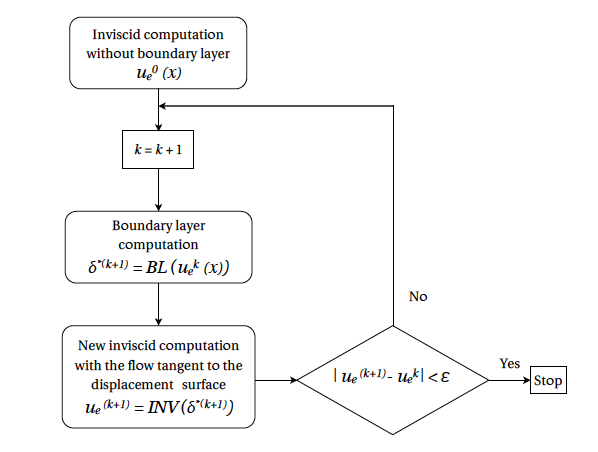
\includegraphics[scale=0.45]{ch5/18}
\captionof{figure}{}
\end{center}

